\documentclass[12pt,a4paper,twoside,openright]{report}
\usepackage{preamble} % imported packages/macros/styling

\usepackage[sorting=nty]{biblatex}
\addbibresource{references.bib}

\begin{document}

\renewcommand{\quote}{\list{}{\rightmargin=\leftmargin\topsep=0pt}\item\relax}

% Reduce align spacing
% \setlength{\abovedisplayskip}{8pt}
% \setlength{\belowdisplayskip}{8pt}
% \setlength{\abovedisplayshortskip}{8pt}
% \setlength{\belowdisplayshortskip}{8pt}

%TC:ignore

% ----------------------------------------------------------------------

% title page 
\pagestyle{empty}

\rightline{\LARGE \textbf{Ellie Vitanov}}

\vspace*{30mm}
\begin{center}
	\Huge
	\textbf{Building an IPv6 Router in P4} \\[20mm]

	\vspace{-2mm}
	
\includegraphics[scale=0.5]{./figures/crest.png}
	\hspace{0mm}\\[20mm]
	\vspace{2mm}


	\LARGE
	Computer Science Tripos -- Part II \\[1mm]
	Churchill College \\[20mm]

	\Large
	\today
\end{center}

\newpage
\thispagestyle{empty}

% ----------------------------------------------------------------------

\pagestyle{plain}

\pagenumbering{roman}


% declaration of originality
\section*{Declaration}

I, Ellie Vitanov of Churchill College, being a candidate for Part II of the Computer Science Tripos, hereby declare that this dissertation and the work described in it are my own work, unaided except as may be specified below, and that the dissertation does not contain material that has already been used to any substantial extent for a comparable purpose. In preparation of this dissertation I did not use text from AI-assisted platforms generating natural language answers to user queries, including but not limited to ChatGPT. I am content for my dissertation to be made available to the students and staff of the University.

\emph{Signed:} Ellie Vitanov\\
\emph{Date:} \today

% proforma
\chapter*{Proforma}
 {\large
  \begin{tabular}{ll}
	  Candidate number:   & 2362D                                        \\
	  Project Title:      & \bf Building an IPv6 Router in P4 \\
	  Examination:        & \bf Computer Science Tripos -- Part II, 2024  \\
	  Word Count:         & 11885\footnotemark[1]                           \\
	  Code Line Count:    & 2540\footnotemark[2]                           \\
	  Project Originator: & The Candidate and Prof. Andrew Moore          \\
	  Project Supervisor: & Prof. Andrew Moore                            \\
  \end{tabular}
 }
\footnotetext[1]{This word count was computed using {\texttt{texcount}}.}
\footnotetext[2]{This code line count was computed using {\texttt{cloc}}}
\stepcounter{footnote}

\section*{Original Aims of the Project}
The aim of this project is to implement an IPv6 router prototype in P4, a domain-specific language for controlling packets, and on the platform P4Pi, a software-based platform which can be run on a general-purpose device. The core objective is for IPv6 packets to be correctly identified and forwarded to the appropriate subnet. Project extensions are to implement additional IPv6 functionalities, such as ICMPv6 and Neighbour Discovery Protocol (NDP), and to provide support for both IPv4 and IPv6 packets.

\section*{Work Completed}
All core objectives and the majority of extensions were completed. The IPv6 router prototype supports parsing, longest prefix table matching, forwarding, two ICMPv6 informational messages, two ICMPv6 error messages, and two NDP messages. The dual-stack router prototype can identify and process both IPv4 and IPv6 packets. The evaluation focused on showing correctness, adherence to networking standards, and that performance in the network is not significantly impacted regardless of whether an example IPv4, the project IPv6, or the project dual-stack router prototype is used.

\section*{Special Difficulties}

None.

% table of contents 
\tableofcontents


% ----------------------------------------------------------------------
\newpage
\pagenumbering{arabic}
\setcounter{page}{1}
%TC:endignore


%TC:envir minted 1 xall 
%TC:envir algorithmic 1 xall

% Include tables in word count
%TC:envir table 0 word
%TC:envir tabular 1 word

% Include footnotes in word count
%TC:macro \footnote [text]
%TC:macro \footnotetext [text]

% main chapters
\addtocontents{lol}{\protect\vspace*{10pt}}
\chapter{Introduction}
%TC:envir minted 1 xall 
%TC:envir algorithmic 1 xall

% Include tables in word count
%TC:envir table 0 word
%TC:envir tabular 1 word

% Include footnotes in word count
%TC:macro \footnote [text]
%TC:macro \footnotetext [text]

%TC:group minted 0 0
%TC:macro \mintinline [ignore]
%TC:macro \colb [ignore]
%TC:macro \hyperref [ignore]

\label{sec:1}

The Internet is made up of heterogeneous physical devices running heterogeneous software applications, all trying to interact with each other. This communication is made possible by the unification of data streams in the network layer of the Internet, where information gets routed according to an Internet Protocol (IP). The main focus of the Internet layer is providing maximum reachability. Regardless of the top-level application or bottom-level physical medium being used, every packet gets routed using an IP in the network layer. The shape of the Internet is thus often described as an hourglass, as shown in \cref{fig:intro-hourglass}. 

\begin{figure}[htbp]
  \centering
    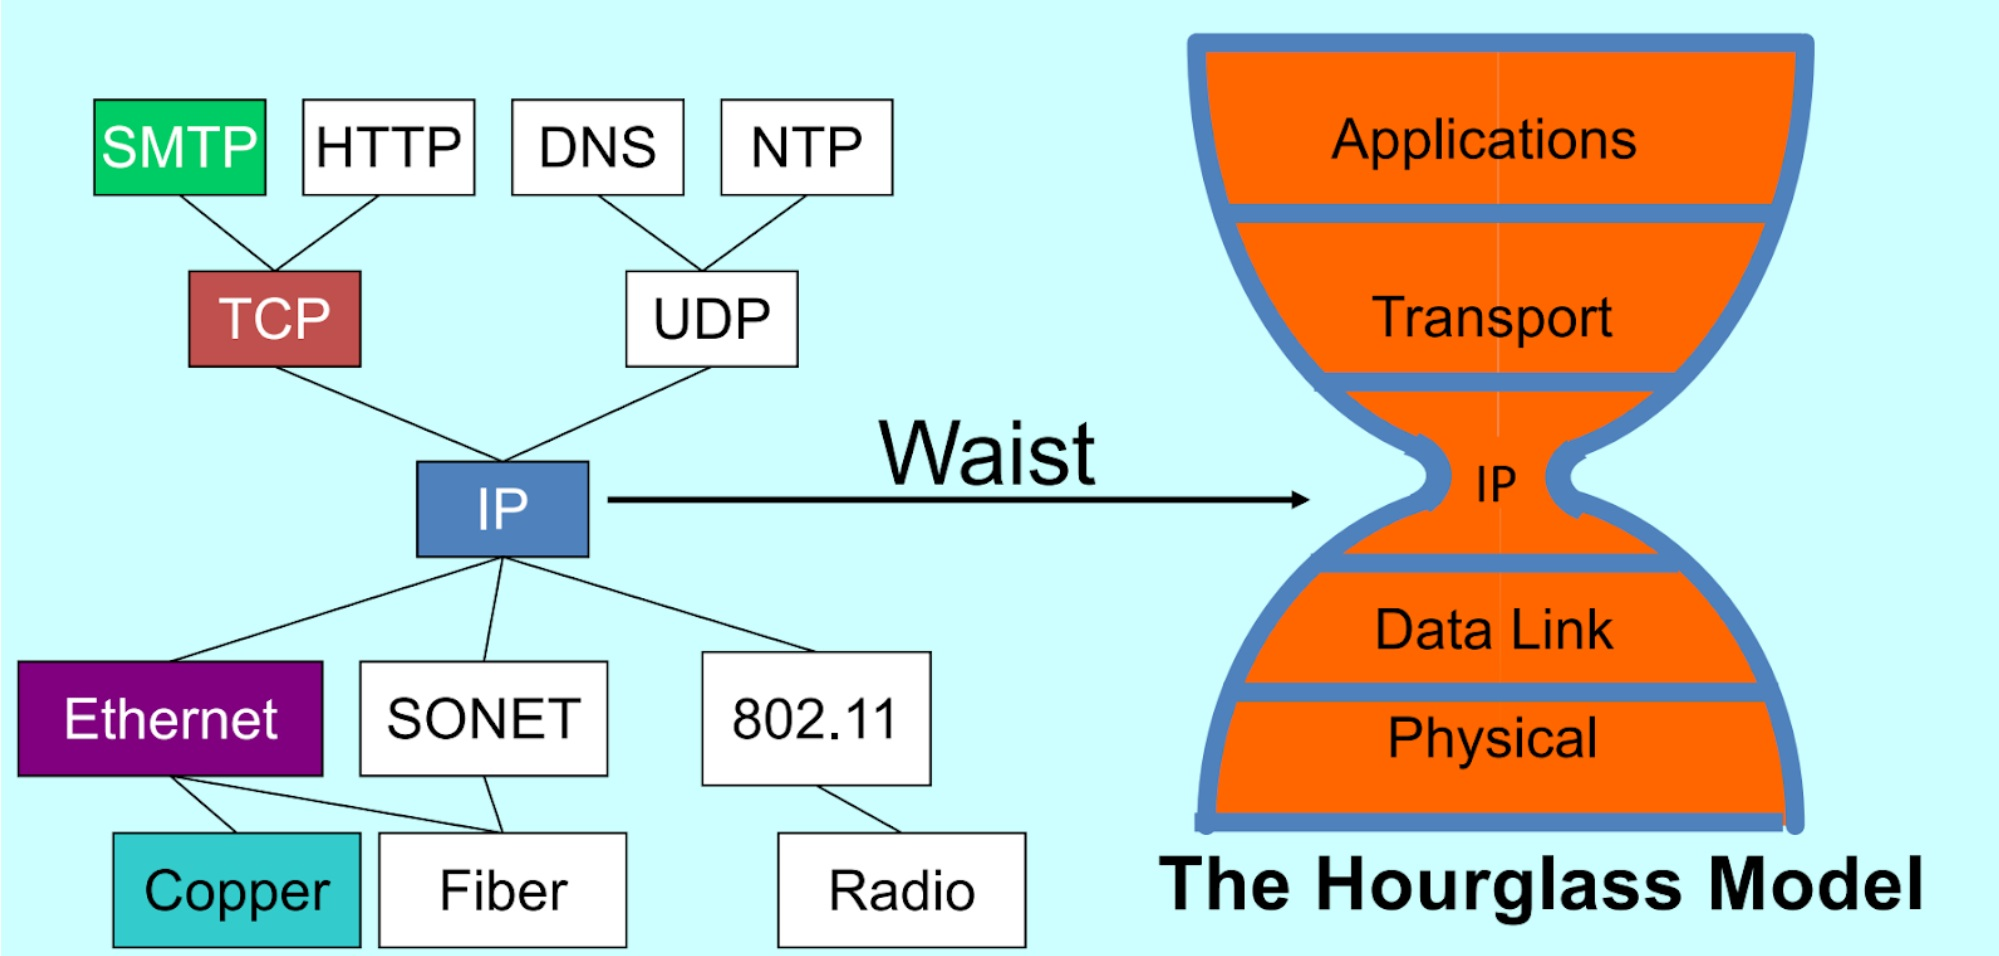
\includegraphics[width=0.65\textwidth]{figures/introduction/hourglass.jpg}
     \caption{The Internet hourglass. Taken from \cite{lectures}.}
     \label{fig:intro-hourglass}
\end{figure}

An IP defines a set of rules that packets need to abide by in order to travel through a network. Upon connecting to the Internet, each node is assigned a unique IP address that allows other devices to locate it anywhere in the world. 

All nodes on the Internet abide by a contract which defines header formats, addressing configurations, datagram structures, and packet handling conventions. Two protocols are currently used in the network layer: IPv4 and IPv6. These protocols coexist in the global Internet, but are mutually incompatible, creating challenges for the migration to one unified IP \cite{lectures}.

IPv4 was released in 1978 and became the globally-accepted Internet standard by the early 1980s \cite{IPv4}. An IPv4 address is 32 bits long and the size of an IPv4 header can vary from 20 to 60 bytes \cite{lectures}. As the Internet started growing exponentially in the late 1980s, IPv4 was anticipated to face an address-space exhaustion problem \cite{IPv6}.  An IPv4 address allows for approximately $2^{32}$ = 4.3 billion unique IP addresses, which was deemed insufficient. This motivated the creation of IPv6, formalised in 1998, which updated the length of an IP address to 128 bits, quadruple the length of an IPv4 address \cite{IPv6}. The address space was hugely increased to $2^{128}$, solving the address-space exhaustion problem \cite{IPv6Paper}. The IPv6 header, which is 40 bytes in length, has been simplified to contain fewer fields than the IPv4 header. A comparison of the two header formats is illustrated in \cref{fig:intro-headers}.

\begin{figure}[htbp]
  \centering
    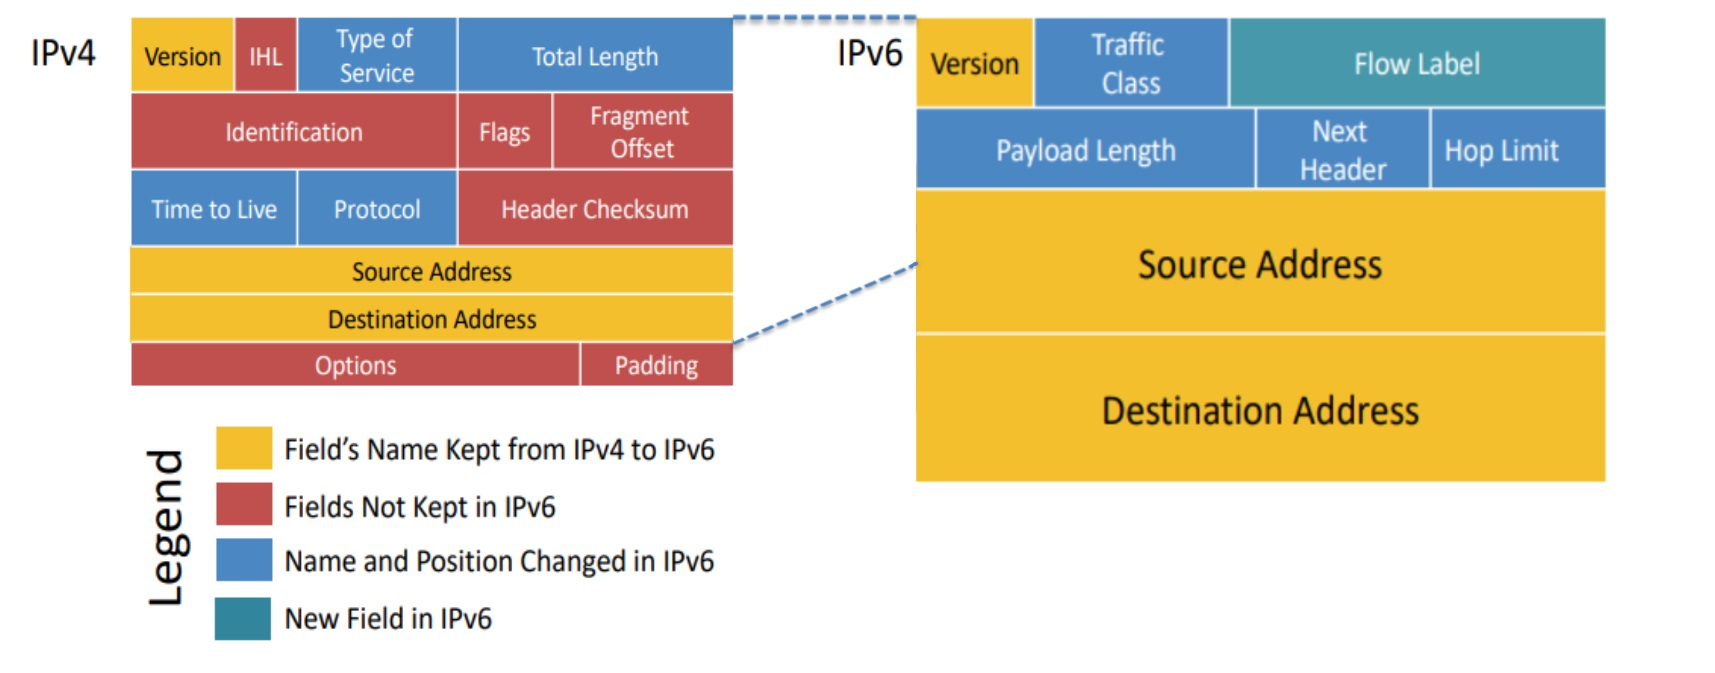
\includegraphics[width=1\textwidth]{figures/introduction/ipv46.jpg}
     \caption{ IPv4 and IPv6 packet header comparison. Adapted from \cite{lectures}.}
     \label{fig:intro-headers}
\end{figure}

Many aspects of the two protocols are incompatible, such as the maximum packet size, fragmentation support, and associated node discovery and diagnostic protocols. IPv4 uses the Address Resolution Protocol (ARP) to discover other nodes on its local network and ICMPv4 for error reporting and signalling. ARP operates below IPv4, while ICMPv4 works on top of IPv4. In IPv6, however, ARP is replaced by the Neighbour Discovery Protocol (NDP), which operates on top of IPv6 and uses ICMPv6 to discover its local network nodes \cite{lectures}.

Due to the various incompatibilities between IPv4 and IPv6, IPv6 adoption rate is still under 50\%, more than 30 years after it was introduced \cite{IPv6Adoption}. Another reason for the low adoption rate is that techniques such as Network Address Translation (NAT) are being used to avoid IPv4's address exhaustion problem. 

A NAT is a device which separates a private network from a public network and allows multiple devices on the private network to access the Internet by using a single public IP address \cite{NAT}. Although this is a widely used workaround, NAT breaks the Internet's end-to-end principle by being a single point of failure (other than the two end hosts) and by requiring information beyond the IP layer (such as port number) to identify nodes in the private network, thus violating security guarantees at the IP level \cite{NATSpecs}. A much more robust solution to the address exhaustion problem would be migrating to IPv6.

Nodes built on IPv4 currently have three options: remain on IPv4, switch to IPv6, or support both. Supporting both IPs can be achieved using various techniques, such as translation, tunneling, or dual IP layering, which are explored in detail in \cref{sec:3.8}. In this dissertation, I refer to a router which implements dual IP layering, i.e. provides separate implementations of both an IPv4 and IPv6 router, as a dual-stack router. Dual-stack nodes bridge the gap between the two IPs and are an essential step in the IPv4-to-IPv6 transition.


\section{Project Summary}
\label{sec:1.1}
The difficulties presented by transitioning from IPv4 to IPv6 motivated my Part II project. I decided to build an IPv6 router on a computer networking platform that does not currently support IPv6. My starting point was the online P4Pi repository, which contains a few example IPv4 functionalities programmed in the domain-specific language (DSL) P4. \cite{P4Pi}. 

In this dissertation I build an IPv6 router prototype, describing in detail the steps I undertake to implement individual functionalities. The core part of my project implements parsing and forwarding in IPv6. Two of the following extensions develop ICMPv6 and NDP functionalities. The final extension examines the nuances involved in extending the router to support both IPv4 and IPv6. This work will highlight the differences between the two IPs and present potential solutions for extending programmable routers to support both.

The evaluation of my project aims to answer the following questions:

\begin{itemize}[topsep=0pt]
\item \textit{Does my router prototype successfully parse, respond to, and forward packets in the manner it was designed to?} At every subtask in Implementation, I state the desired behaviour of the program I am building. I then evaluate the correctness of my programs according to these expectations in \cref{sec:4.1}.

\item \textit{Does my router prototype adhere to Internet Engineering Task Force (IETF) specifications?} In \cref{sec:4.2} I analyze the official technical Internet standards that outline the current best practices for network node behaviour, and I establish that my router prototype adheres to them.

\item \textit{Does the network exhibit significant changes in performance when comparing an IPv4 router, my IPv6 router, and my dual-stack router?} In \cref{sec:4.3} I build a test network and compare the performance of known Internet traffic in both IPs on single- and dual- stack routers to conclude that the difference in efficiency is minimal.

\end{itemize}

\addtocontents{lol}{\protect\vspace*{10pt}}
\chapter{Preparation}
%TC:envir minted 1 xall 
%TC:envir algorithmic 1 xall

% Include tables in word count
%TC:envir table 0 word
%TC:envir tabular 1 word

% Include footnotes in word count
%TC:macro \footnote [text]
%TC:macro \footnotetext [text]

%TC:group minted 0 0
%TC:macro \mintinline [ignore]
%TC:macro \colb [ignore]
%TC:macro \hyperref [ignore]

\label{sec:2}
In preparation for my project, I learned a new programming language P4, explored how this language interacts with a software-defined data plane, studied the P4Pi networking platform, and worked through some provided example P4 programs. In \cref{sec:2.1} I define the notion of a software-defined router and explain why I chose this approach for my project. \cref{sec:2.2} and \cref{sec:2.3} introduce the DSL P4 and the networking platform P4Pi, respectively, and \cref{sec:2.4} explores the different components of the P4Pi platform and how they interact. Finally, \cref{sec:2.5} and \cref{sec:2.6} describe the project's starting point and my requirements analysis.



\section{Software-Defined Networking (SDN)}
\label{sec:2.1}

Software-Defined Networking (SDN) is an approach to network management that decouples the control plane software from the data plane hardware and moves the switch configuration mechanisms to software \cite{SDNPaper}. Network nodes based on this approach use generic hardware, which not only makes switch production easier and cheaper, but means that different network configurations can be built on top of a single piece of hardware. Providing customisable network infrastructure gives system admins control over configurations that were formerly baked into switch hardware \cite{SDN}. \cref{fig:prep-sdn} compares a traditional network and a software-defined network.

\begin{figure}[htbp]
  \centering
    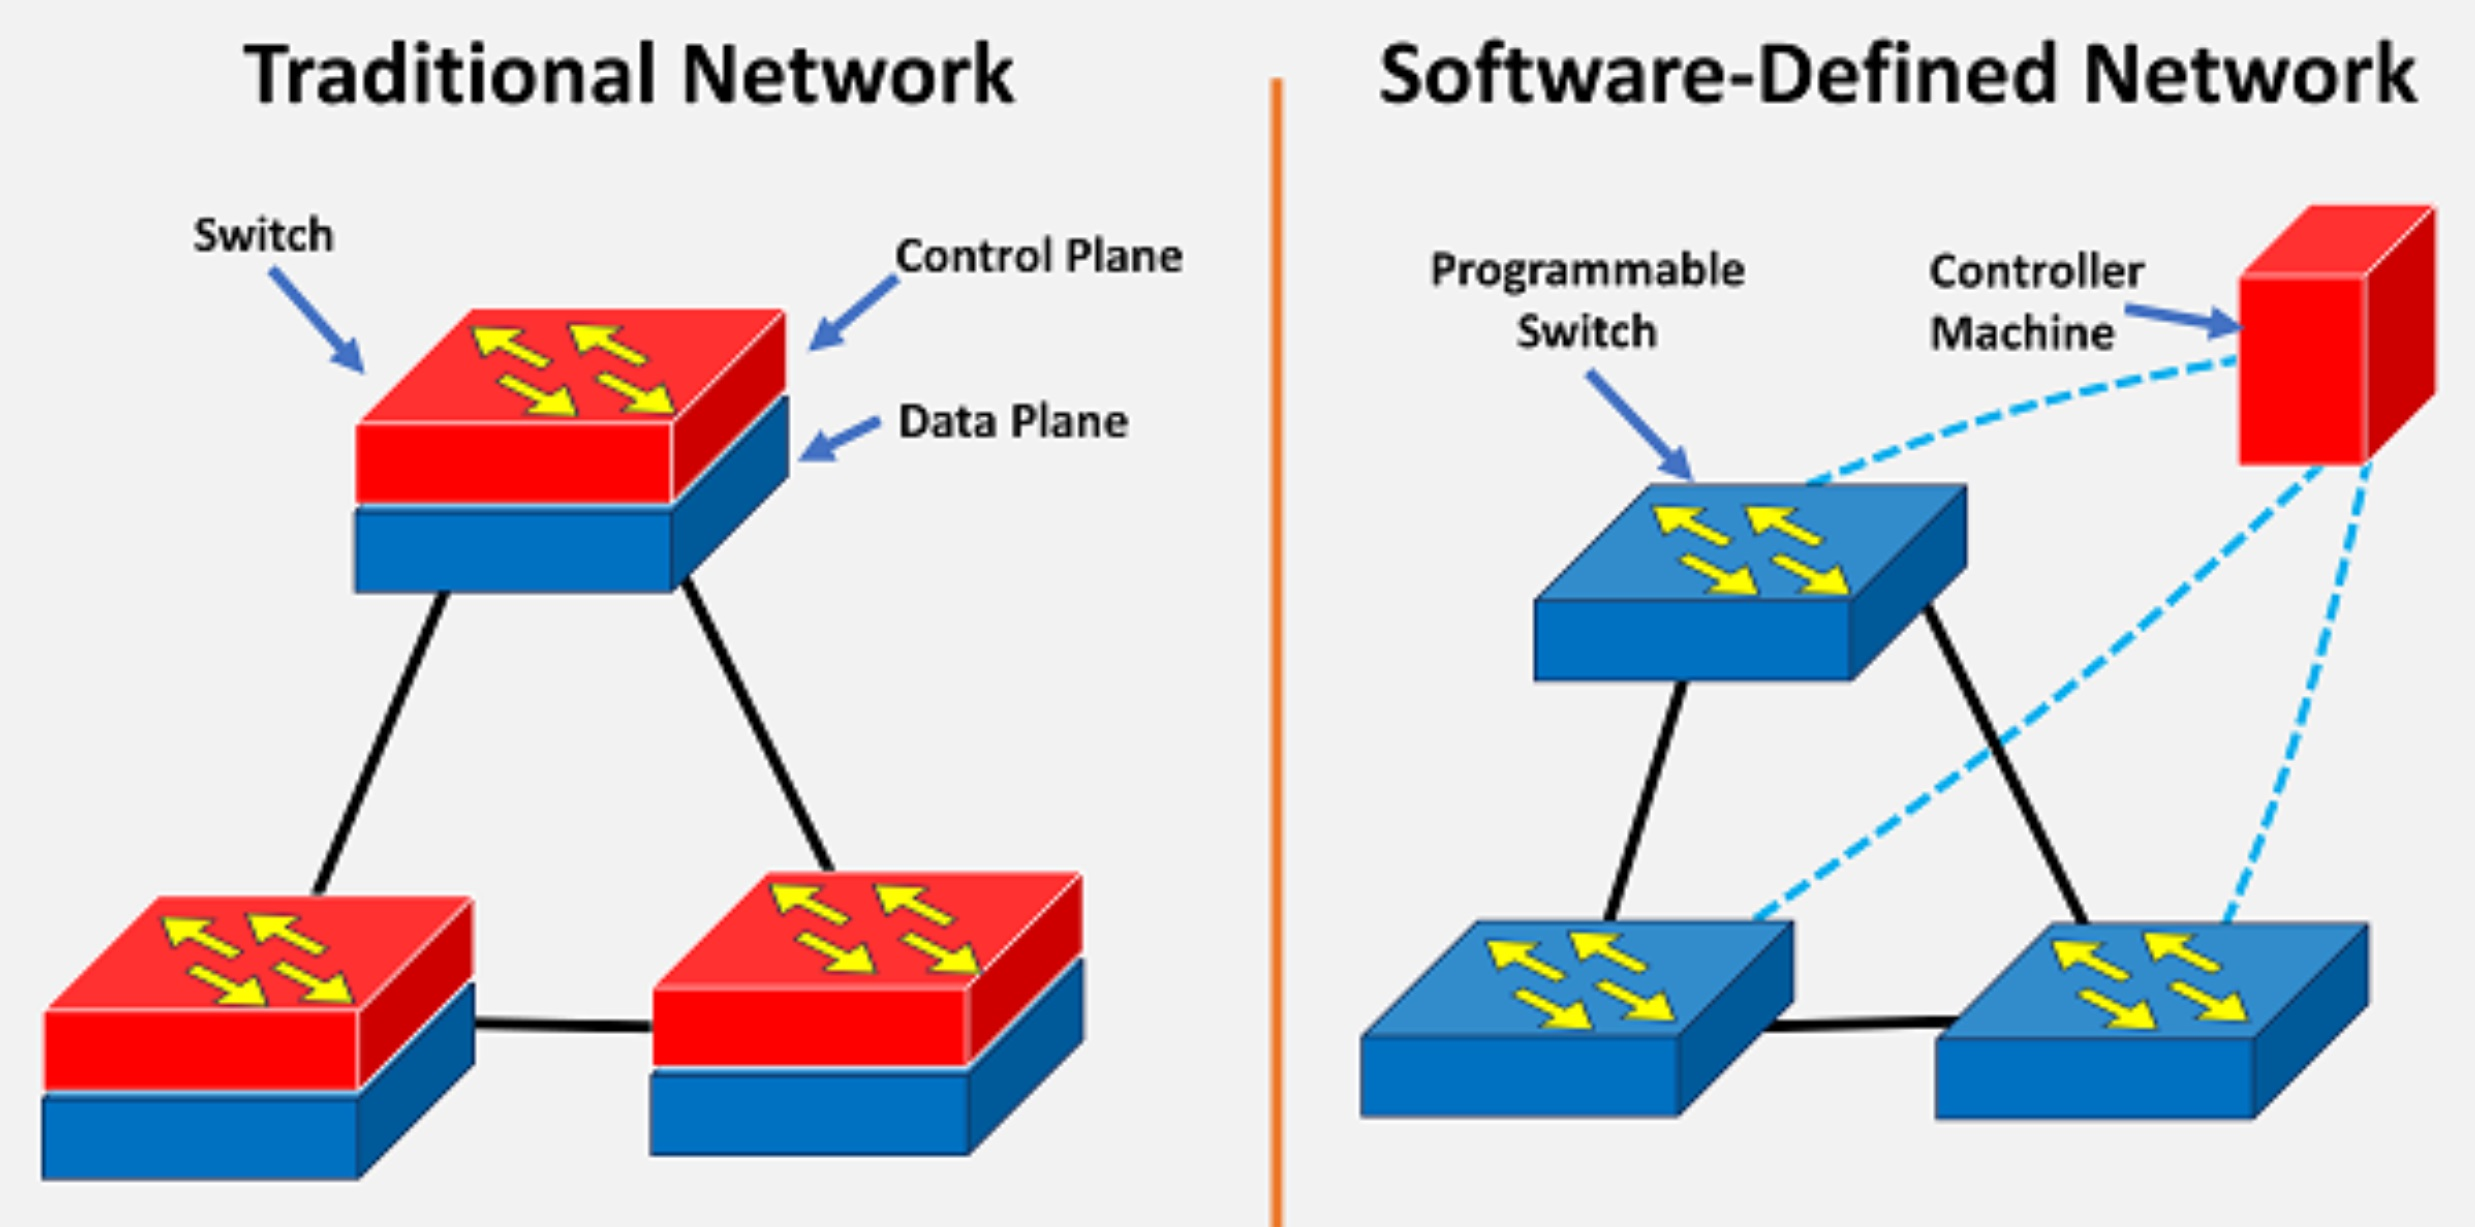
\includegraphics[width=0.8\textwidth]{figures/preparation/sdn.jpg}
     \caption{A comparison between a network consisting of traditional network \\ nodes and software-defined network nodes. Taken from \cite{SDNImage}.}
     \label{fig:prep-sdn}
\end{figure}

I chose to build my router on a software-defined platform because it provides more flexibility, a straightforward implementation pipeline, and real-time reconfiguration of network nodes. This made rerunning P4 code, changing network designs, and testing different data plane configurations much faster and simpler. It is also more affordable, since I  needed a general-purpose device to build my router on top of, rather than a specialised piece of hardware.



\section{P4 as a Network DSL}
\label{sec:2.2}
For my project, I chose the domain-specific language (DSL) P4 \cite{P4Paper}. P4 defines how packets are processed in the data planes of forwarding nodes, such as switches and routers. In accordance with the P4 language specifications, a packet-processing system capable of running P4 code is a P4 ‘target’, and a set of P4-programmable blocks are a P4 ‘architecture’ \cite{P4LangSpecs}.

P4 introduces a novel way of programming SDN nodes, which is flexible, expressive, and portable. The language can define data plane configurations of varying complexity to be run on a general-purpose target that does not have any fixed functionalities or knowledge of network protocols. A P4 program can be run on any target that supports the chosen architecture, regardless of the vendor that has produced it \cite{P4LangSpecs}.

P4 uses a set of core abstractions: header types, parsers, tables, actions, match-action units, and others. Functional blocks in the language can take three distinct parameter types: \texttt{in}, \texttt{inout} and \texttt{out}. The \texttt{in} parameter type is an immutable input; the \texttt{out} parameter type is initially undefined and can be written to; and the \texttt{inout} parameter type is a combination of both, i.e. initially defined and can be modified.

P4 uses most common data types, such as \texttt{void}, \texttt{int}, \texttt{string} and \texttt{bool}, along with \texttt{match\_kind} for table matching. It uses the types \texttt{bit<i>} and \texttt{int<i>} to define fixed-length variables of width \texttt{i}, as well as \texttt{varbit<i>} to define a variable of width between \texttt{0} and \texttt{i}. There are also a number of derived data types, such as \texttt{enum}, \texttt{header}, \texttt{header union}, \texttt{parser}, and \texttt{control} \cite{P4LangSpecs}. An example \texttt{control} block declaration is shown in \cref{fig:prep-matchaction}.

\begin{figure}[htbp]
  \centering
    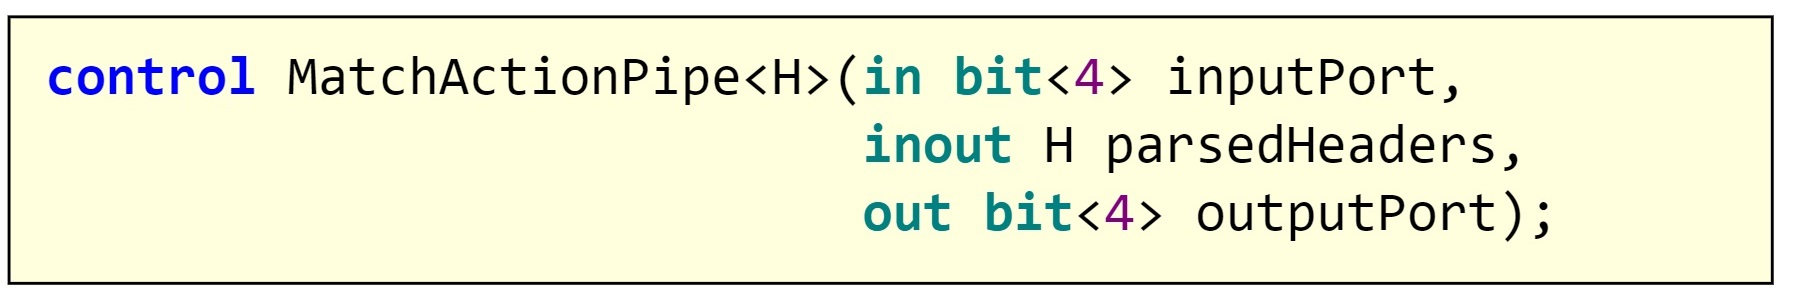
\includegraphics[width=0.7\textwidth]{figures/preparation/match_action.jpg}
     \caption{An example P4 control block declaration. Adapted from \cite{P4LangSpecs}.}
     \label{fig:prep-matchaction}
\end{figure}

A \texttt{header}, representing a packet header, is a collection of fields placed in a defined order. Headers need to have a maximum size, thus each field is either of type \texttt{bit<i>} or \texttt{varbit<i>}. If a header does not contain any \texttt{varbit<i>} type fields, then it is a fixed-size header, an example of which is shown in \cref{fig:prep-ethernet}. A \texttt{header union} represents a disjunction of multiple different headers, any of which could be placed at a point in the program where the header union is used.

\begin{figure}[hbtp]
  \centering
    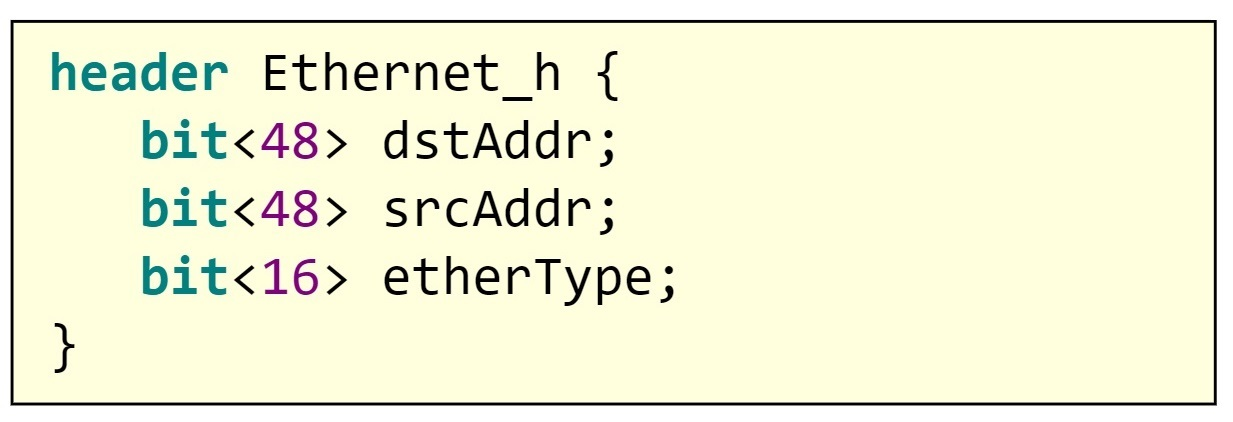
\includegraphics[width=0.5\textwidth]{figures/preparation/ethernet.jpg}
     \caption{An example Ethernet header. Adapted from \cite{P4LangSpecs}.}
     \label{fig:prep-ethernet}
\end{figure}

When a packet is being processed by a P4 program, it goes through three main stages: the \texttt{parser}, which extracts headers; the \texttt{match-action} pipeline, which manipulates the extracted headers; and the \texttt{deparser}, which prepends the updated headers. There are many ways that this pipeline can be further expanded upon, and in this dissertation I have additionally implemented \texttt{checksum verification} and \texttt{checksum update} stages.

A \texttt{parser} is a state machine with one starting state, \texttt{start}, and two final states, \texttt{accept} and \texttt{reject}. Each state is made up of statements that extract headers, lookup header fields and, optionally, define a transition to a different state. Accepted packets continue to the processing stages of the pipeline, whereas rejected packets are dropped. Parsers require an additional parameter type \texttt{packet\_in}, which represents the packet that has just entered the pipeline before headers are extracted. \cref{fig:prep-parser} is a \texttt{parser} declaration with one input and two outputs.

\begin{figure}[htbp]
  \centering
    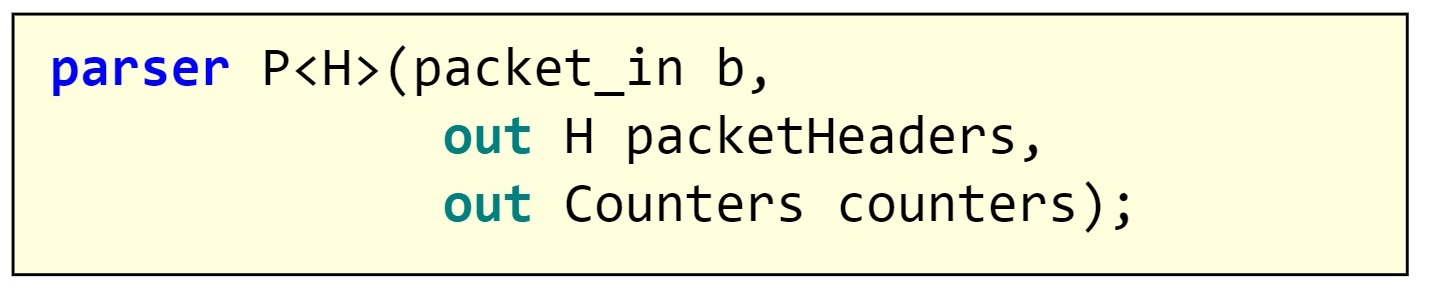
\includegraphics[width=0.55\textwidth]{figures/preparation/parser.jpg}
     \caption{An example \texttt{parser} declaration. Adapted from \cite{P4LangSpecs}.}
     \label{fig:prep-parser}
\end{figure}

A \texttt{control} block is a functional block used to manipulate headers extracted by the parser. It is made up of an \texttt{application} block, which defines the packet's control flow, \texttt{action} blocks, and \texttt{table} blocks. Actions are used to read and write processed data, whereas tables describe \texttt{match-action} units, i.e. units where a header field is matched to a table key to decide which action to take next. Each table entry consists of a key, an action ID and action data. Entries are checked from top to bottom, and if a match is encountered, the corresponding action is performed. A table for IPv4 forwarding using longest prefix match is shown in \cref{fig:prep-table}.

\begin{figure}[htbp]
  \centering
    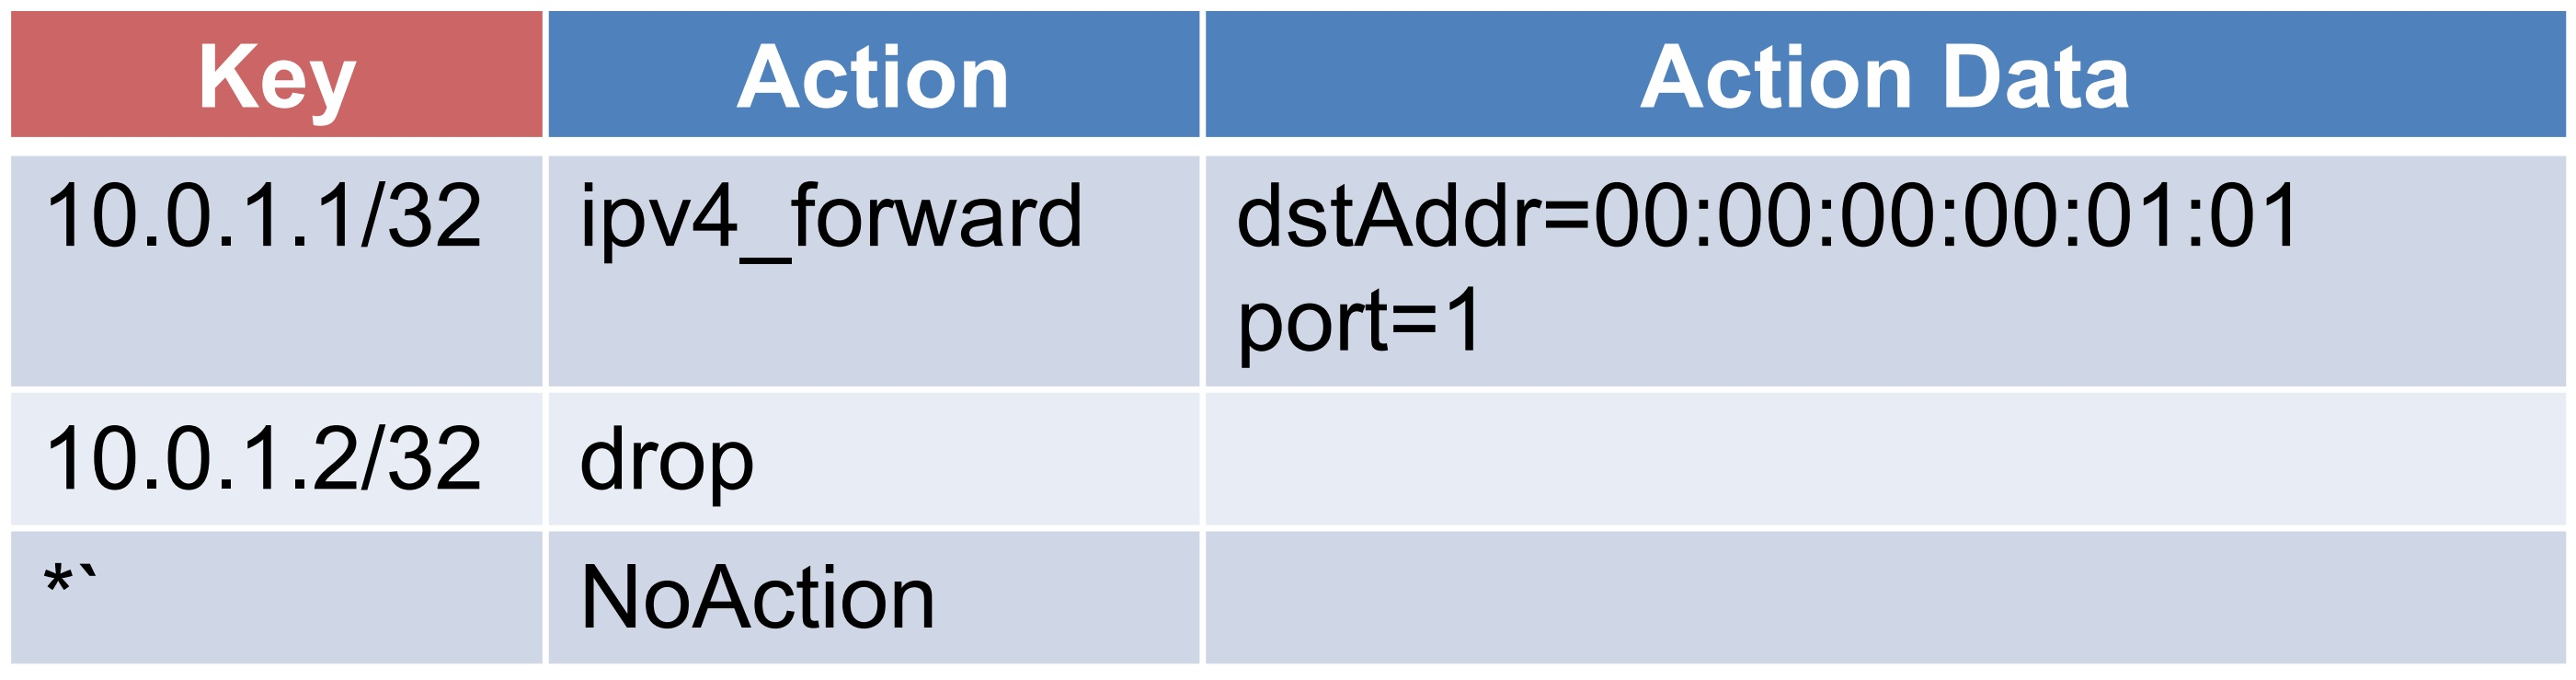
\includegraphics[width=0.55\textwidth]{figures/preparation/ipv4_table.jpg}
     \caption{An example \texttt{match-action} table. Taken from \cite{P4LangTutorial}.}
     \label{fig:prep-table}
\end{figure}

The \texttt{deparser} does not have its own derived type and is instead also performed in a \texttt{control} block, with the additional requirement that it must contain at least one parameter of type \texttt{packet\_out}. Similarly to how \texttt{packet\_in} represents the packet that has just arrived at the node, \texttt{packet\_out} defines the reconstructed packet that is sent back out into the network.

My project will not require any further P4 knowledge, but the language provides a wide variety of tools to build sophisticated packet control flow configurations beyond what I have discussed.



\section{P4Pi as an SDN Platform}
\label{sec:2.3}
P4Pi is an open source platform implemented on Raspberry Pi devices, which allows prototyping with P4. It provides an affordable hands-on method for research in the field of networking \cite{P4Pi}. The platform is available in a GitHub repository, which contains instructions on how to set up, install and configure the target \cite{P4Pi}. The repository defines a framework for running and testing P4 programs, which is outlined in \cref{sec:2.4} and also provides a few simple tutorials \cite{P4Pi}. I learned how to manipulate headers, perform table lookups, forward/drop packets, and use the Runtime Shell to dynamically update data plane tables.

I chose to conduct my project on this platform for multiple reasons: the required equipment is affordable and was available at the department; it is portable, which meant I could take it home and work on the project over the breaks; and most importantly, it allowed me to build a network of separate devices to route and track packets through, which helped me analyse the intricacies of a multi-host network. 



\section{Programming Framework}
\label{sec:2.4}

Programming a P4 target requires an understanding of how the different components of a packet-switching device interact with P4 code. \cref{fig:prep-framework} shows the stages a P4 program goes through before it runs on a target.

\begin{figure}[htbp]
  \centering
    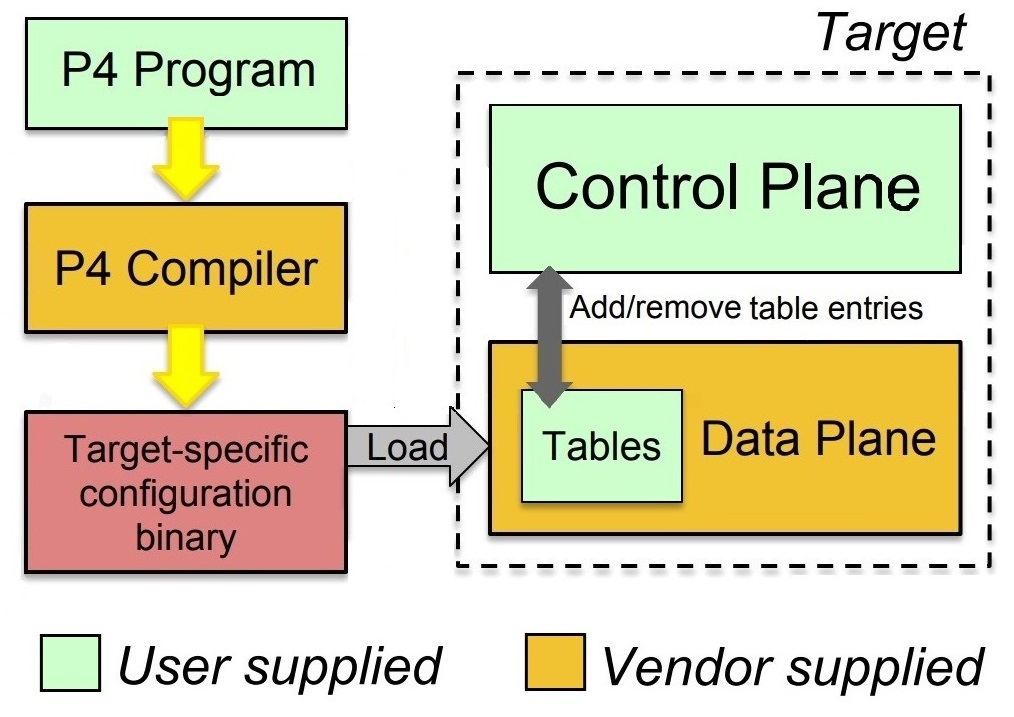
\includegraphics[width=0.5\textwidth]{figures/preparation/programming_target.jpg}
     \caption{Programming a P4 target. Adapted from \cite{P4LangTutorial}.}
     \label{fig:prep-framework}
\end{figure}

Every P4 program has to be written based on a defined architecture model, and every target has to abide by the behavioural model of a reference software switch. I define these notions in \cref{sec:2.4.1} and \cref{sec:2.4.2}, respectively. I describe how the P4 compiler produces a target-interpretable version of a P4 program in \cref{sec:2.4.3}, how it defines a control plane API in \cref{sec:2.4.4}. Finally, in \cref{sec:2.4.5}, I comment on how P4Pi interacts with external components, such as packet generators and packet sniffers.



\subsection{\textit{V1Model} Architecture}
\label{sec:2.4.1}

In my project, all P4 programs have been written abiding by the \textit{V1Model} architecture \cite{V1model}. A P4 architecture model defines a software template of a P4 program. In the V1Model, every program is made up of eight blocks of code: header definitions, parser, checksum verification, ingress processing, egress processing, checksum update, deparser, and a switch definition. All P4 code written by the user goes into one of these blocks and each function is required for the code to compile \cite{V1model}. \cref{fig:prep-v1arch} shows a simplified version of the packet processing pipeline defined by the \textit{V1Model}, and \cref{fig:prep-v1code} shows a P4 program structure split into the aforementioned eight code blocks. Each pipeline stage in \cref{fig:prep-v1arch} corresponds to one or more code block in \cref{fig:prep-v1code}.

\begin{figure}[htbp]
  \centering
    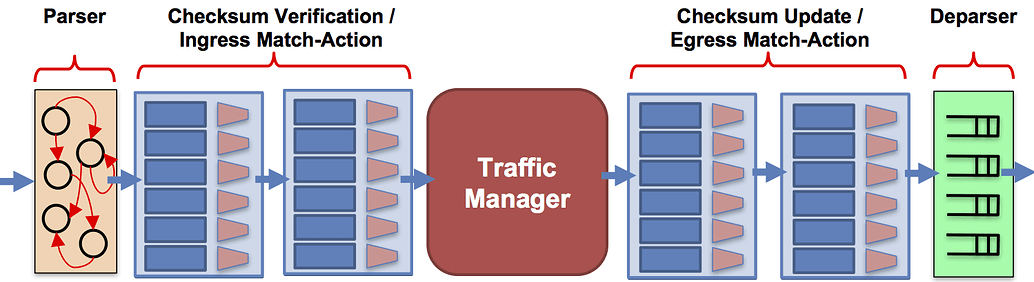
\includegraphics[width=0.8\textwidth]{figures/preparation/v1model_architecture.png}
     \caption{\textit{V1Model} pipeline. Taken from \cite{P4LangTutorial}.}
     \label{fig:prep-v1arch}
\end{figure}

\begin{figure}[htbp]
  \centering
    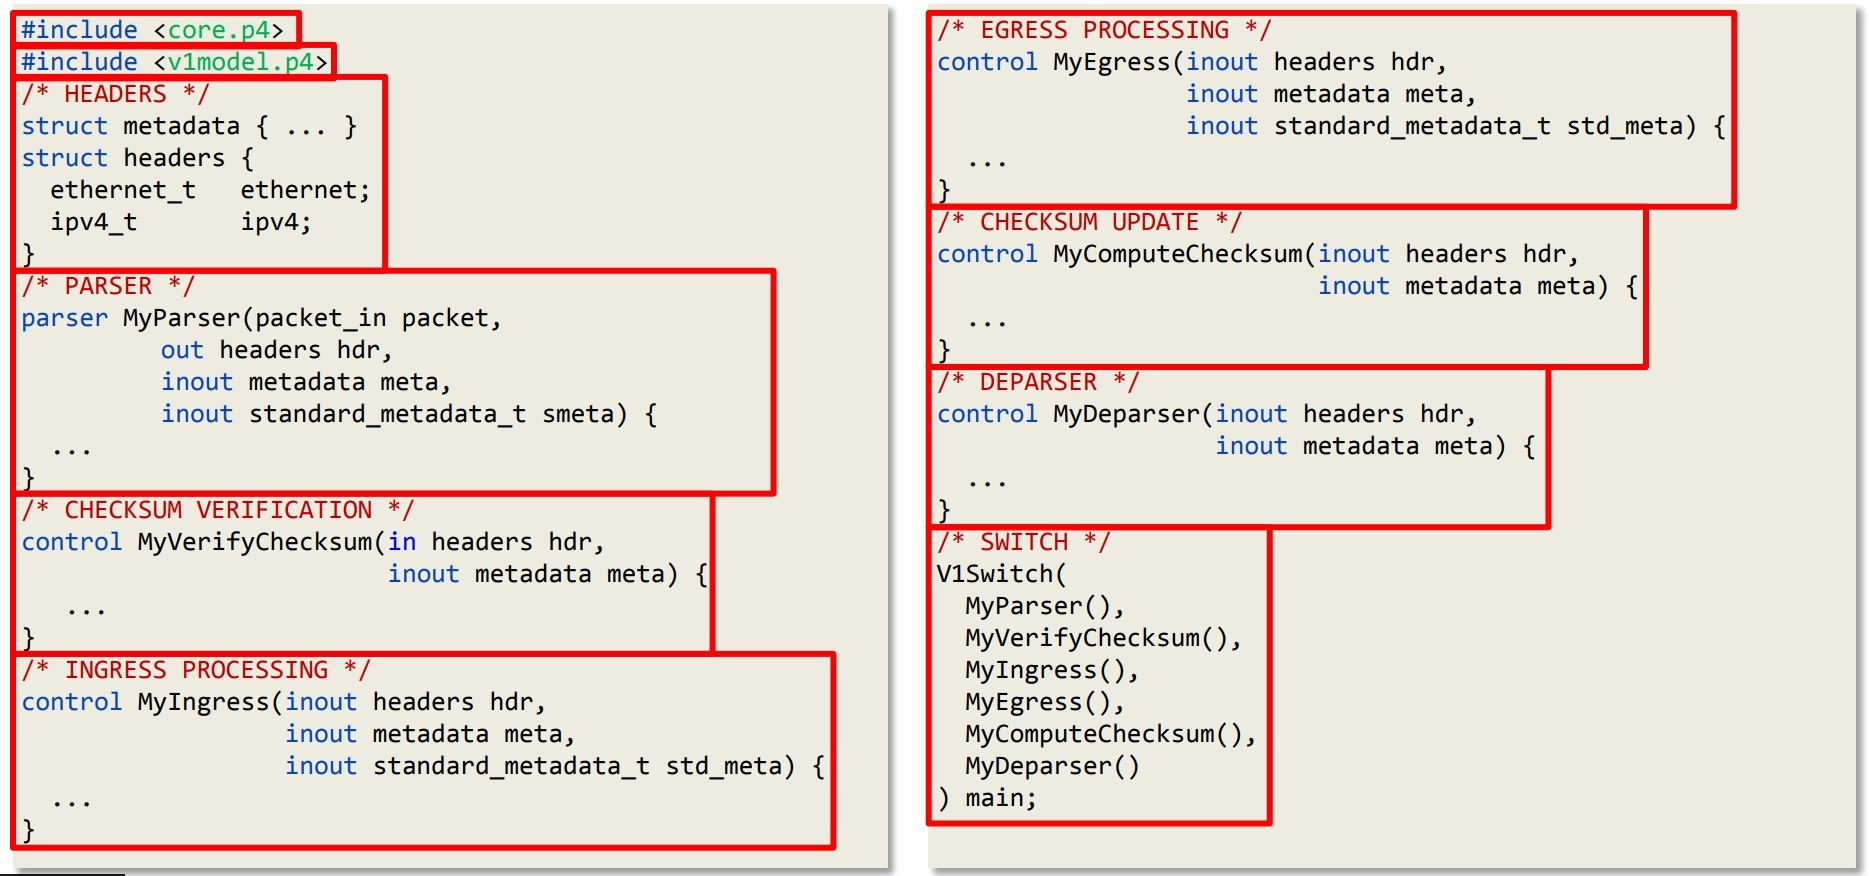
\includegraphics[width=0.8\textwidth]{figures/preparation/v1model_template.jpg}
     \caption{\textit{V1Model} code template. Taken from \cite{P4LangTutorial}.}
     \label{fig:prep-v1code}
\end{figure}



\subsection{\textit{Simple Switch} Target}
\label{sec:2.4.2}

I chose the \textit{simple switch} target for my project because it runs on a general-purpose CPU and offers all necessary functionalities. The \textit{simple switch} target is an implementation of the abstract \textit{BMv2} reference P4 software switch \cite{BMv2}. \textit{BMv2} is an abstract switch, i.e. it provides the necessary resources (such as how much memory is available) for a target to be implemented, but does not define a target implementation (e.g. using the memory to implement registers) \cite{P4LangTutorial}. The \textit{simple switch} target implements ingress and egress (de)parsers and control, as well as counters, actions, a checksum function, packet buffers with replication engines, and many more. It also offers runtime support for updating the control plane without requiring recompilation of the P4 program \cite{BMv2target}. \cref{fig:prep-relation} shows the relationship between a P4 program, the \textit{V1Model} architecture model, the \textit{simple switch} target implementation, and the \textit{BMv2} behavioural model.

\begin{figure}[htbp]
  \centering
    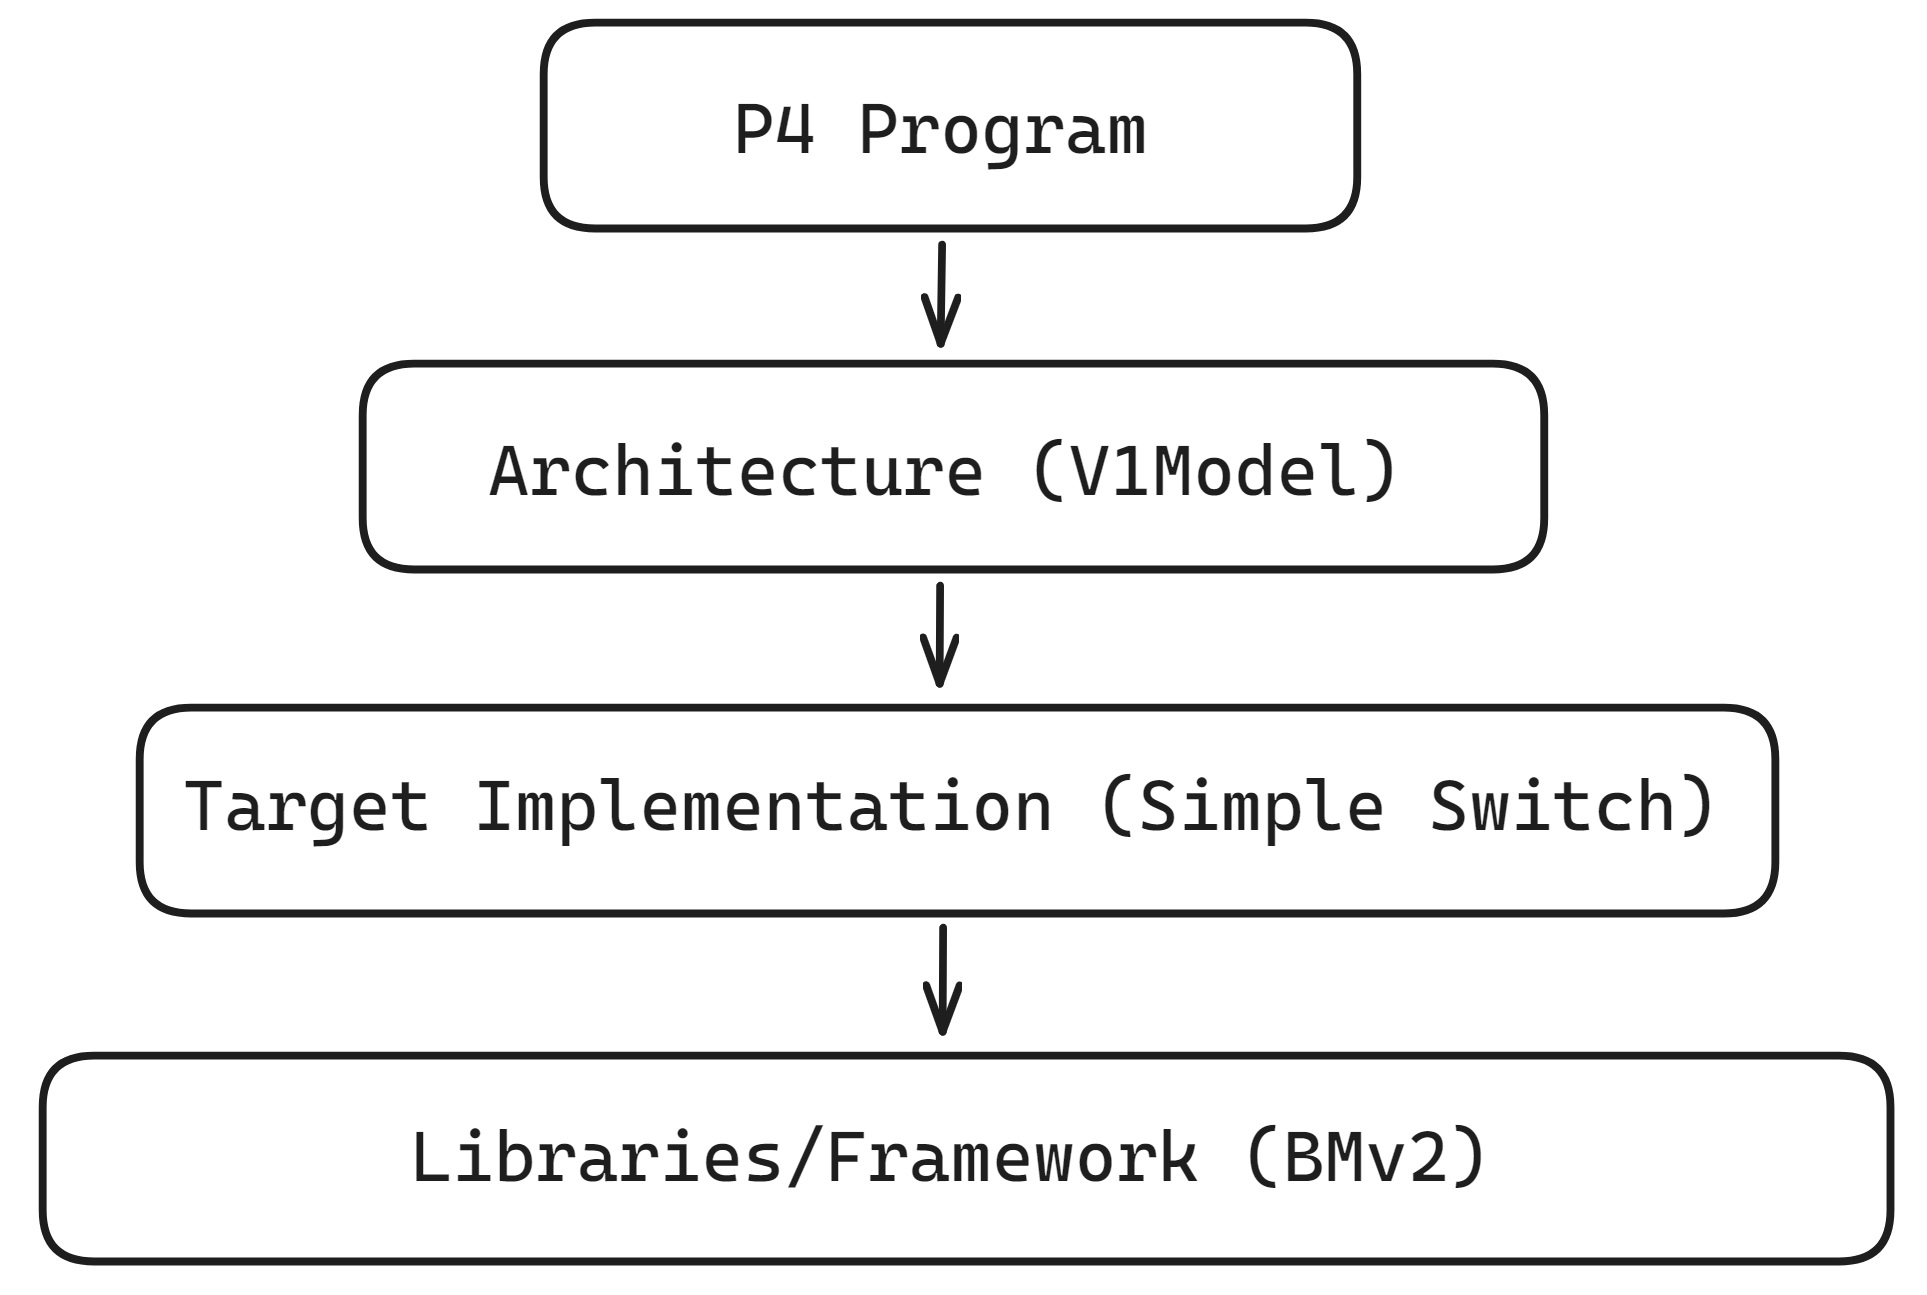
\includegraphics[width=0.45\textwidth]{figures/preparation/control_flow.jpg}
     \caption{Relating concepts. Adapted from \cite{P4Architecture}.}
     \label{fig:prep-relation}
\end{figure}



\subsection{P4 Compiler}
\label{sec:2.4.3}

The default reference compiler for the P4 language is \textit{p4c}, which provides a standardised modular frontend and midend for the compiler. To produce a fully-functional P4 Compiler, \textit{p4c} must be combined with a target-specific backend. The provided backend for the \textit{simple switch} target is \textit{p4c-bm2-ss} \cite{P4Compilers}.

The \textit{simple switch} P4 compiler takes four arguments:
\begin{itemize}[topsep=0pt]
\item \textit{BMv2} – the abstract switch model;
\item \textit{v1Model} – the architecture model;
\item \texttt{p4-16} – the P4 version the program was written in;
\item a \texttt{.p4} file – the P4 program to be compiled;
\end{itemize}

and outputs two files:
\begin{itemize}[topsep=0pt]
\item \texttt{.p4i} – contains the preprocessor output;
\item \texttt{.json} – data plane configurations in the file format \textit{BMv2} targets require as input.
\end{itemize}

The \texttt{.json} file can then be run on the \textit{simple switch} target. For more details on how to run a P4 program on the P4Pi platform, see Appendix A \cite{P4Pi}. 

\subsection{\textit{Simple Switch CLI}}
\label{sec:2.4.4}

The target's command line interface, \textit{simple switch CLI} allows dynamic inspection, addition, deletion, and modification of the tables defined by the P4 program. Each table entry consists of a key-action pair where the action tells the switch how to proceed upon a key match. For a brief overview of commands that can be used in the CLI, see Appendix B \cite{P4LangTutorial}.




\subsection{External Components}
\label{sec:2.4.5}

Once a program has been compiled and loaded into the P4Pi switch, it can interact with external components. A packet generator (e.g. Scapy \cite{Scapy}) can be used to send packets to the target. Packets go through the port interface and into the \textit{V1Model} pipeline, where they are manipulated as defined by the P4 program data plane configurations. A packet sniffer (e.g. Wireshark \cite{Wireshark}) can then be used inspect the packets once they have been processed and outputted. Running in parallel, the target's CLI can dynamically update the data plane tables. Changes made through the CLI take effect immediately and new packet processing behaviour is then observed. \cref{fig:prep-overview} illustrates the described interactions.

\begin{figure}[htbp]
  \centering
    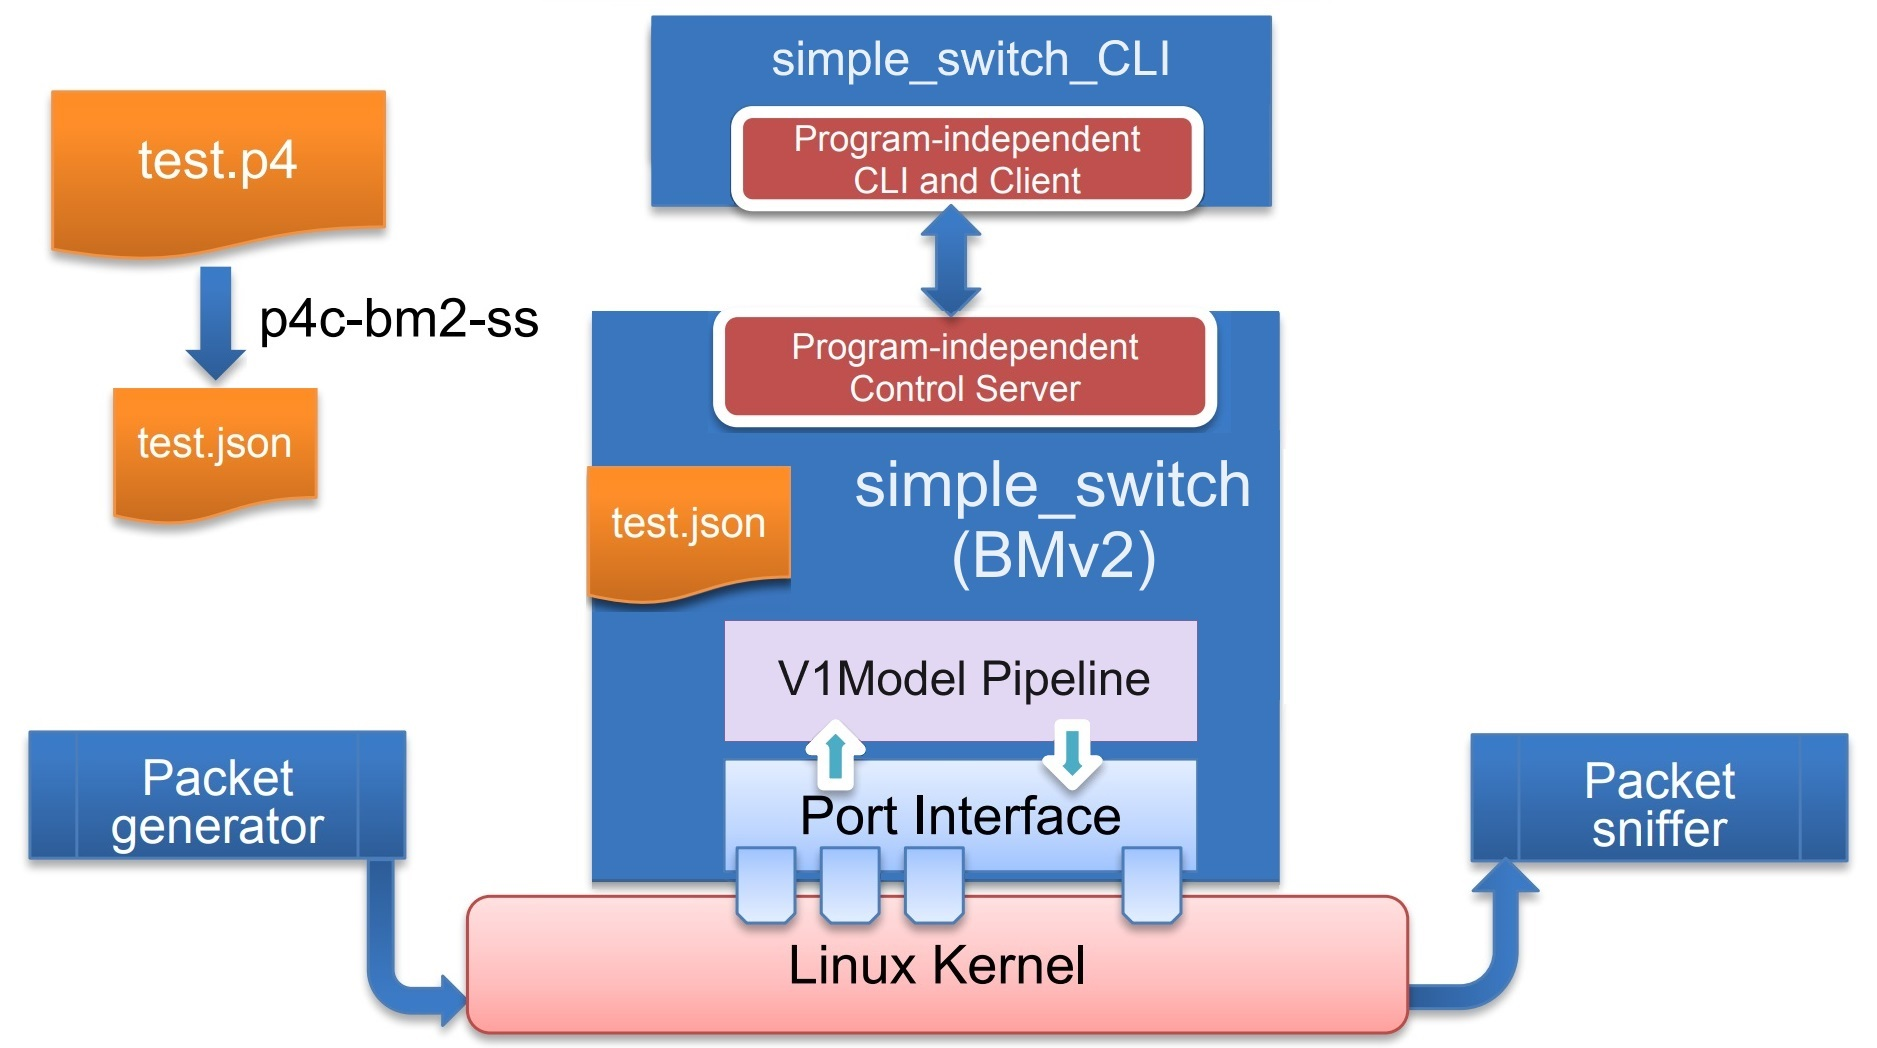
\includegraphics[width=0.8\textwidth]{figures/preparation/overview.jpg}
     \caption{Interaction with external components. Adapted from \cite{P4LangTutorial}.}
     \label{fig:prep-overview}
\end{figure}




\section{Starting Point}
\label{sec:2.5}
The initial P4Pi repository contained a P4 architecture (\textit{V1Model}), a P4 compiler, a P4 target (\textit{simple switch}), a target-specific Runtime Shell (\textit{simple switch CLI}), and some example IPv4 functionalities, such as forwarding, ARP Reply, and Echo Reply.

The aim of my project is to build an IPv6 router prototype. The core objective is for the router to support parsing, header manipulation, and forwarding of IPv6 packets. Two of my extensions are to add ICMPv6 and NDP functionalities (the equivalent of IPv4’s ICMP and ARP, respectively). The final extension takes a simple P4 IPv4 router (adapted from the P4Pi repository) and merge it with my IPv6 router to build a dual-stack router prototype, which can process both IPv4 and IPv6 packets.



\section{Requirements Analysis}
\label{sec:2.6}

My project required hardware, which I obtained from my supervisor: three Raspberry Pis, three SD cards, Ethernet cables, and Ethernet-to-USB adaptors. I occasionally used my college's computer room to set up multiple monitors, mouses, and keyboards in order to attach each Raspberry Pi to its own screen.

I set up a GitHub repository to regularly push all my code to and adhered to P4 standards when writing and formatting my code. I used the iterative agile methodology for code development in order to break down my work into tasks that can be achieved within a fortnight. The project was built using test-driven development. Using the packet analyser Wireshark \cite{Wireshark}, I observed packet formats and exchanges in a working network, and based my router behaviour on them. I used bespoke testing on known test traffic to evaluate the correctness and performance of my P4 programs.

\cref{fig:prep-req} shows all required functionalities, grouped into core objectives and three extensions. This diagram is not intended as a packet dataflow. It is intended to show the dependencies between router components. An arrow from Block A to Block B means that Block A needs to be implemented in order for Block B to work. All tasks have been successfully completed.

\begin{figure}[hbtp]
  \centering
    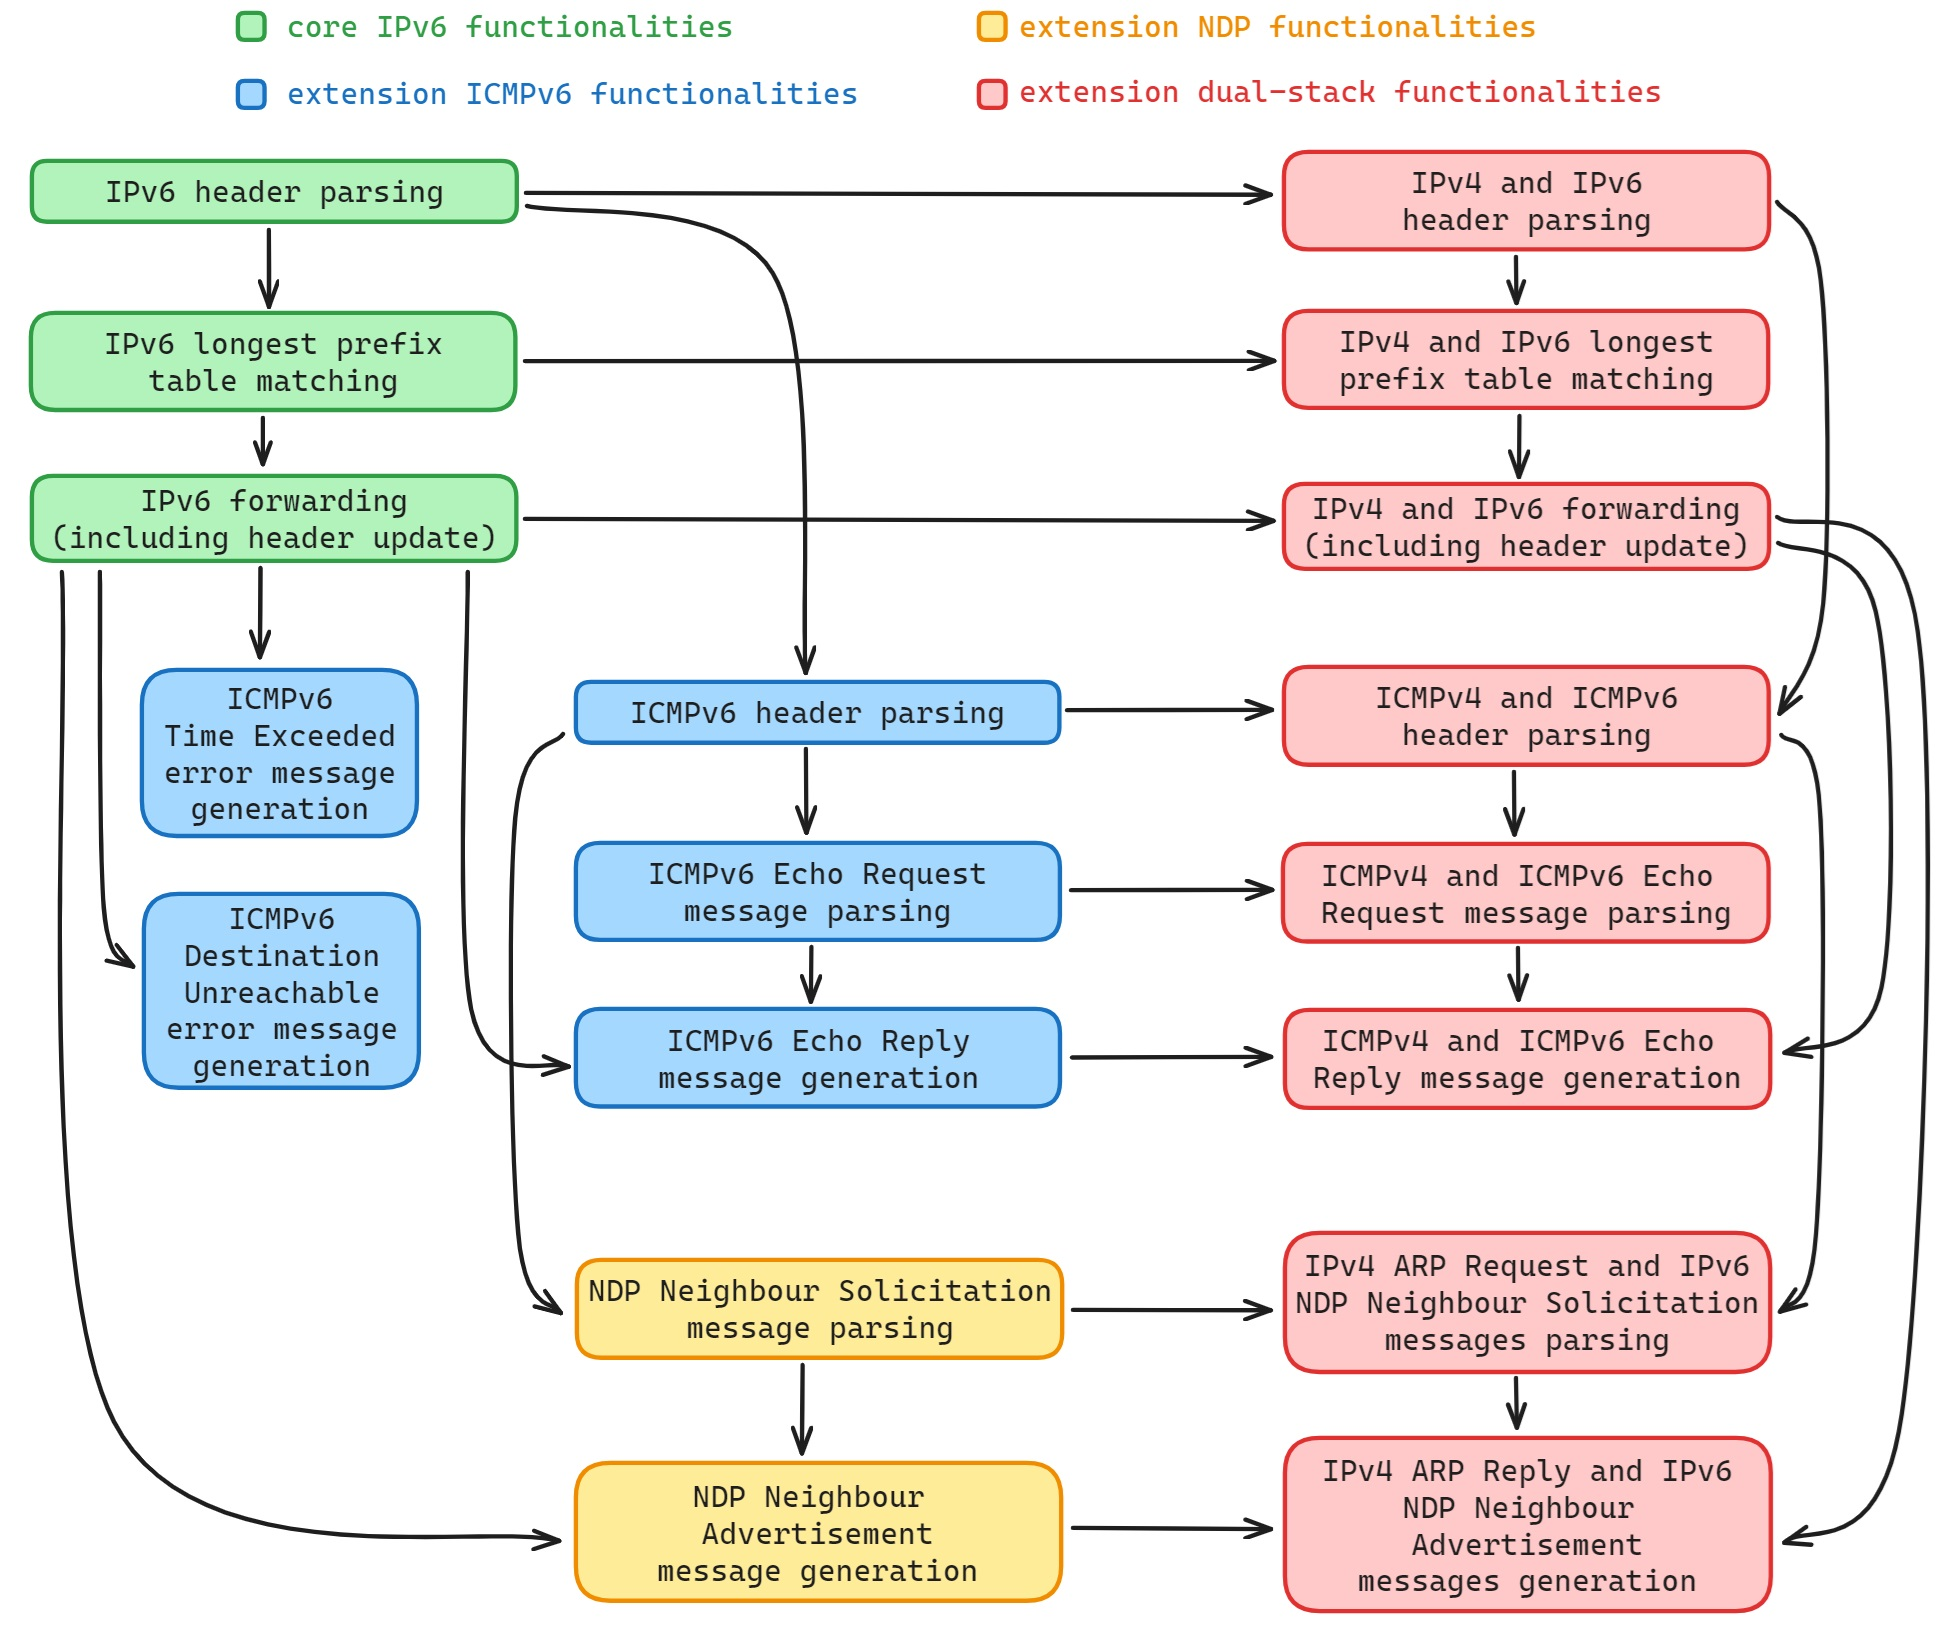
\includegraphics[width=1\textwidth]{figures/preparation/req_analysis.jpg}
     \caption{Dependency diagram between router functionalities.}
     \label{fig:prep-req}
\end{figure}

\addtocontents{lol}{\protect\vspace*{10pt}}
\chapter{Implementation}
%TC:envir minted 1 xall 
%TC:envir algorithmic 1 xall

% Include tables in word count
%TC:envir table 0 word
%TC:envir tabular 1 word

% Include footnotes in word count
%TC:macro \footnote [text]
%TC:macro \footnotetext [text]

%TC:group minted 0 0
%TC:macro \mintinline [ignore]
%TC:macro \colb [ignore]
%TC:macro \hyperref [ignore]

\label{sec:3}

The implementation of this project consists of three distinct steps: programming individual IPv6 router functionalities; merging them together into a single program to implement a full IPv6 router prototype; and adding an IPv4 stack to the router to support dual IP layering. By completing these objectives, I fulfill the core part of my project, along with three of the proposed extensions.

\cref{sec:3.1}, \cref{sec:3.2}, and \cref{sec:3.3} contain network setup, code repository and implementation overviews, respectively. In \cref{sec:3.4} I describe building a router that can parse and forward IPv6 packets. In \cref{sec:3.5} and \cref{sec:3.6} I implement ICMPv6 and NDP functionalities, respectively. These separate components are ultimately assembled in \cref{sec:3.7} to create a full IPv6 router prototype. 

In \cref{sec:3.8}, I discuss different mechanisms that could be used to support both IPv4 and IPv6 and explain why I chose dual IP layering. For the final part of my project, in \cref{sec:3.9}, I merge my IPv6 router with a simple IPv4 router prototype, in order to present a dual-stack router prototype. To aid with reproducibility, some of the sections have corresponding appendices that describe the configurations and commands for each node.



\section{Network Setup}
\label{sec:3.1}

All my experiments use three Raspberry Pis: two acting as hosts and one acting as the router. I connect both hosts to the router using Ethernet cables, as shown in the diagram. The two colours represent the two different subnets the hosts belong to. The router has two statically defined IPv6 addresses: one for each subnet. The statically defined MAC addresses match those of the Raspberry Pi’s respective Ethernet-to-USB adaptor ports. \cref{fig:impl-setup} shows the described setup.

I assign static IPv6 addresses to both hosts (based on the subnet of the respective router port) and define routes to all devices in the network. The P4 program configurations are loaded into the P4Pi data plane. The control plane is handled by the CLI, which I use to populate the table entries in the P4 programs, as necessary.

For the dual-stack router, I also add static IPv4 addresses to both hosts and the router. Additional setup differs depending on the specific experiments, and is discussed in the following sections, as well as in each experiment’s respective appendix. 

\begin{figure}[htbp]
  \centering
    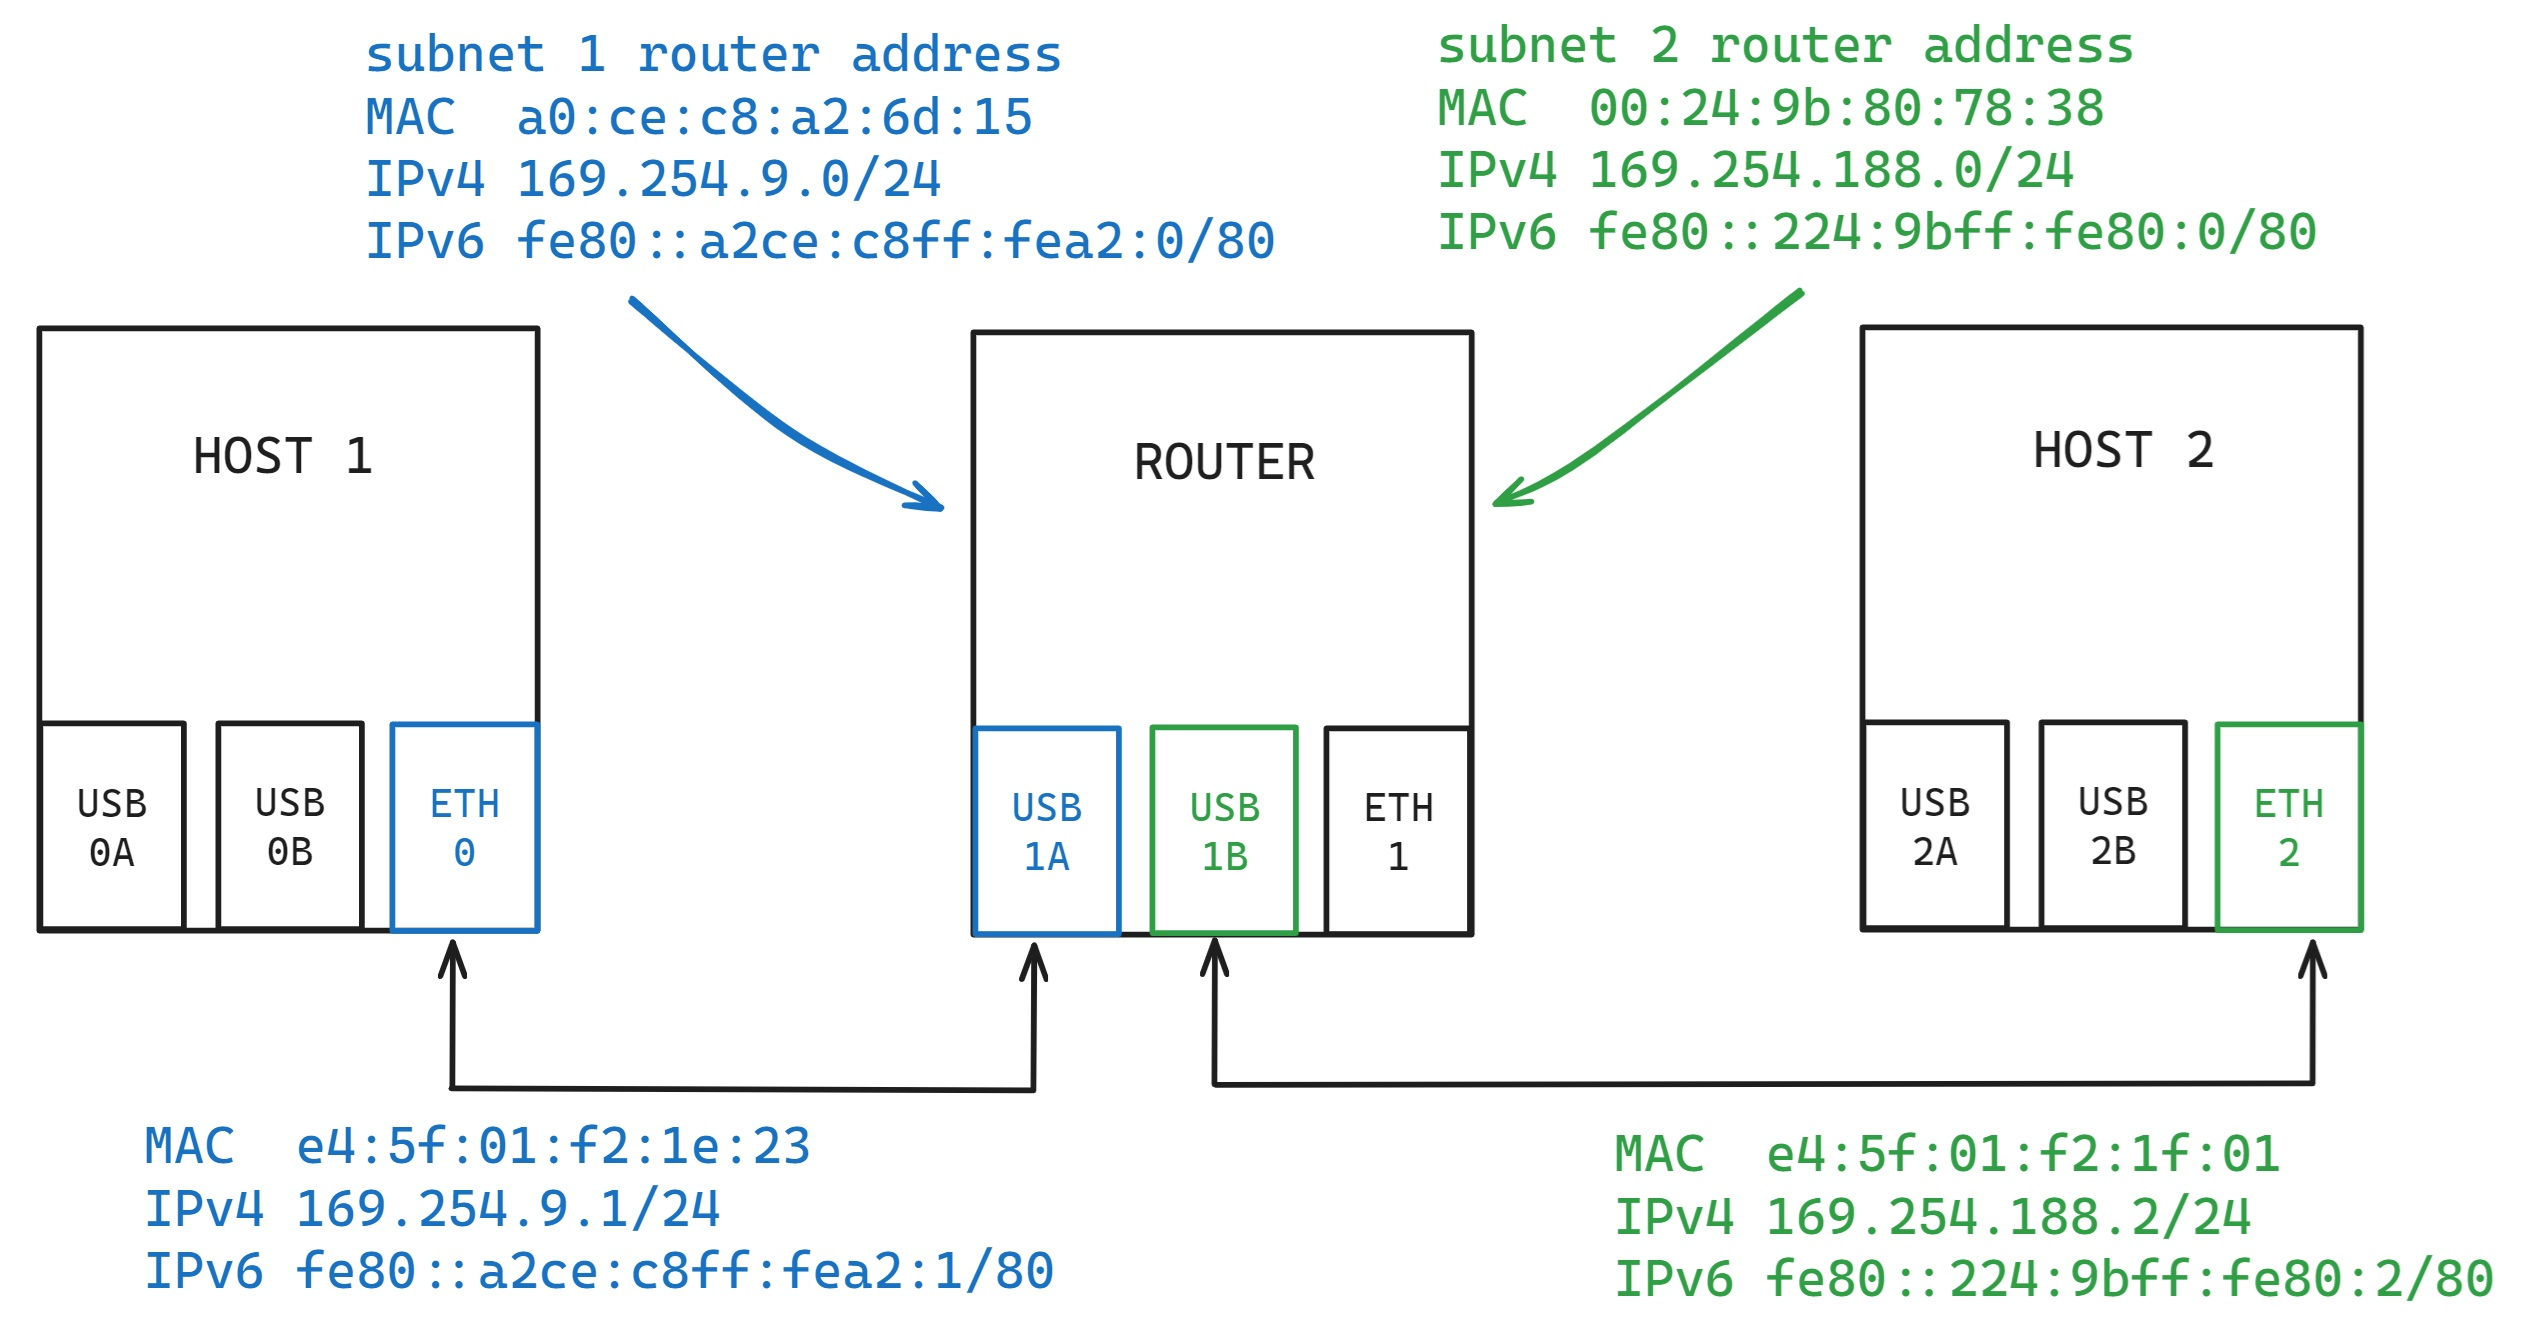
\includegraphics[width=0.85\textwidth]{figures/implementation/setup.jpg}
     \caption{Raspberry Pi setup for the router experiments.}
     \label{fig:impl-setup}
\end{figure}

\pagebreak

\section{Repository Overview}
\label{sec:3.2}

There are a total of eight folders in my code repository, along with a \texttt{README} file. Six of the folders contain a \texttt{.p4} file with the P4 program implementing data plane functionalities, usually along with \texttt{.txt} files with commands to populate the tables in the P4 program through the CLI (effectively acting as the control plane). The seventh repository folder has a Python script I used to plot the graphs in \cref{sec:4.3}. The final repository folder contains the \texttt{LaTeX} source code for my dissertation write up.

\bigskip

\dirtree{%
.1 partii\_dissertation.
.2 README.md.
.2 ipv6 \DTcomment{\textbf{core:} IPv6 forwarding}.
.3 ipv6.p4.
.3 commands.txt.
.2 icmpv6 \DTcomment{\textbf{extension 1:} ICMPv6 functionalities}.
.3 icmpv6.p4.
.2 ndp \DTcomment{\textbf{extension 2:} NDP functionalities}.
.3 ndp.p4.
.3 commands.txt.
.2 router4 \DTcomment{integrates IPv4 functionalities from P4Pi repository}.
.3 router4.p4.
.3 commands.txt.
.2 router6 \DTcomment{integrates IPv6 functionalities from core, extensions 1 and 2}.
.3 router.p4.
.3 commands.txt.
.2 dualstack \DTcomment{\textbf{extension 3:} merges IPv4 and IPv6 functionalities}.
.3 dualstack.p4.
.3 commands.txt.
.2 figures \DTcomment{plots of gathered evaluation data}.
.3 figures.ipynb.
.3 .png files.
.2 dissertation \DTcomment{dissertation source code}.
}

\pagebreak

\section{Implementation Process}
\label{sec:3.3}

I build my IPv6 router prototype using an incremental approach. I implement P4 programs that support independent functionalities, test them in isolation, and then add them to the router. Every P4 program adheres to the \textit{V1Model} architecture model, as outlined in \cref{sec:2.4.1}.

A program adhering to the \textit{V1Model} is comprised of eight distinct code blocks: the header definitions; six packet-processing pipeline stages (parser, checksum verification, ingress processing, egress processing, checksum update, and deparser); and the switch definition. It is not necessary to use all pipeline stages in order to implement a functionality. For example, IPv6 does not use checksums, so those code blocks would be left empty. There are a few characteristics that all my programs share:

\textbf{Ingress Processing} ~ Ingress processing is made up of three different functional blocks: table matchings, actions, and the application block. The application block defines a control flow that decides which action is applied to a packet based on its header fields. Some packets have a table matching performed on a certain header field in order to determine which action is applied to them. Actions include manipulating header fields, choosing egress ports, or simply dropping the packet.

\textbf{Egress Processing} ~ Egress processing is structured the same way as ingress processing. The reason they are separate pipeline stages is that packets that are cloned, recirculated, or generated by the control plane only go through egress processing. For the purposes of this project, all packets go through ingress processing, so I do not require separate egress processing. This pipeline stage is therefore left empty, and I do not mention it again in the following sections.

\textbf{Switch Definition} ~ In every program, the switch definiton takes the six pipeline stage functions as arguments in order to produce a P4 \textit{V1Model} software switch configuration.

In each of the following sections, I describe a functionality design and implementation. I base my designs on observed packet behaviour in a working home network and developed my router such that it mimics the behaviour of my home router. All program logic is my own work.



\section{IPv6 Forwarding}
\label{sec:3.4}

The core objective of my project is to implement the necessary components of an IPv6 router: parsing and forwarding. My P4 program parses an incoming packet, does a longest prefix match on the destination address, and, if there is a table hit, forwards the packet to a specified port.



\subsection{IPv6 Header Packet Format}
\label{sec:3.4.1}

The IPv6 header format is 40 bytes long and made up of 8 fields, as shown in \cref{fig:impl-ipv6header}. For the purposes of this project, aside from the Destination Address field, I reference the Next Header field, used to identify the type of payload being carried by the packet, and the Hop Limit field, used to indicate when a packet has exceeded the amount of nodes it is allowed to visit in the network before it is dropped. The packet's payload is appended to the end of the IPv6 header.

\begin{figure}[htbp]
  \centering
    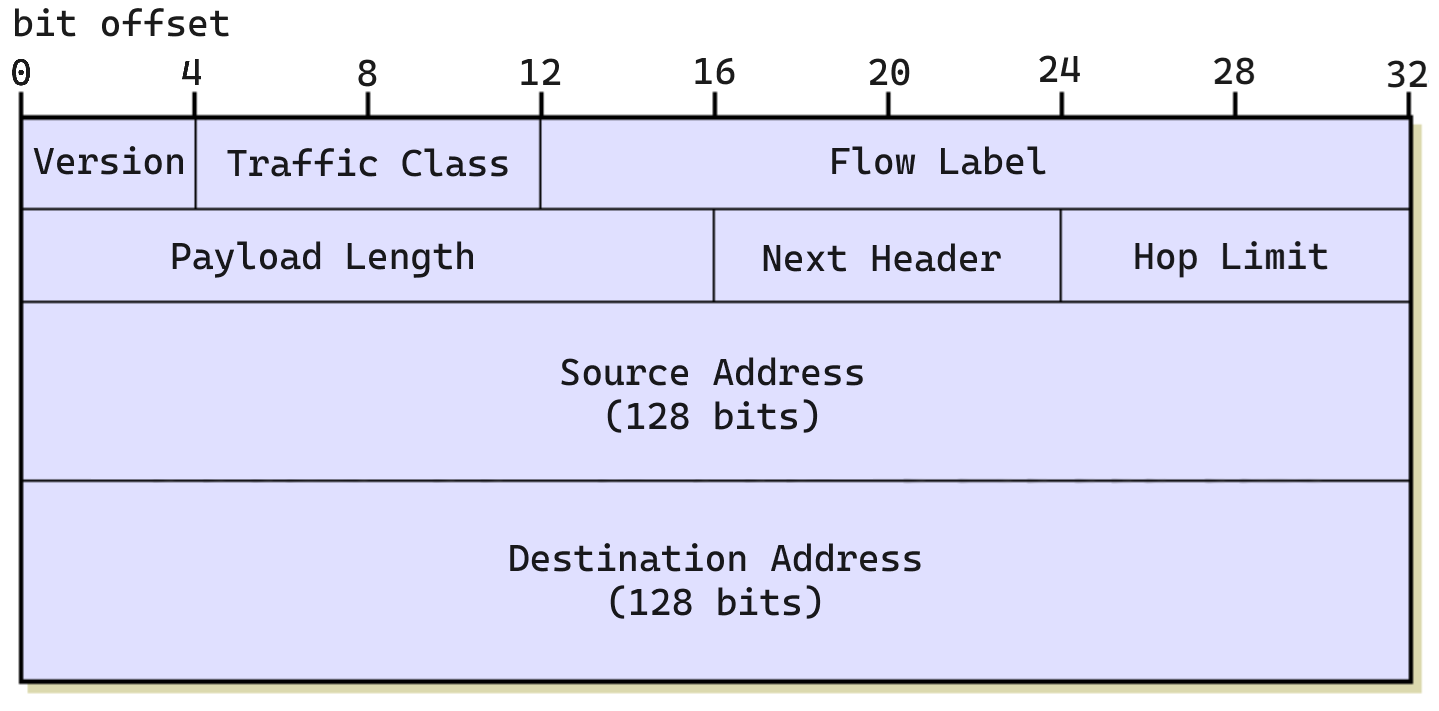
\includegraphics[width=0.55\textwidth]{figures/implementation/ipv6_header.png}
    \caption{IPv6 header format. Adapted from \cite{IPguide}.}
    \label{fig:impl-ipv6header}
\end{figure}



\subsection{IPv6 Forwarding Design}
\label{sec:3.4.2}

Once the data plane is configured, I populate the IPv6 forwarding table using the CLI. The entries use IPv6 addresses as keys, which match to a next-hop MAC address and a port output number. A packet sent from Host 1 is forwarded by the router towards Host 2, and vice versa. No packet loss or duplication is observed. For more detailed information on how to run this experiment, consult Appendix C.



\subsection{IPv6 Forwarding Program}
\label{sec:3.4.3}

The data plane behaviour of the router is specified by the P4 file \texttt{ipv6.p4}. 

\textbf{Header Definitions} ~ I define two header types: a 14-byte Ethernet header, which contains a source MAC address, a destination MAC address, and a Type field; and a 40-byte IPv6 header, which contains Version, Traffic Class, Flow Label, Payload Length, Next Header, and Hop Limit fields, together with a source and destination IPv6 address.

\textbf{Parser} ~ The parser filters incoming packets based on their headers. This program’s parser state machine has two intermediary states: one for parsing Ethernet headers and one for parsing IPv6 headers, as shown in \cref{fig:impl-ipv6parser}. The \texttt{start} state automatically transitions to the \texttt{Ethernet} state, where the Ethernet header is extracted and a check is performed, testing whether the next header is of type IPv6. If it is, the state machine transitions to the \texttt{IPv6} state. There it extracts the IPv6 header and moves on to the next stage of the \textit{V1Model} pipeline.

\begin{figure}[htbp]
  \centering
    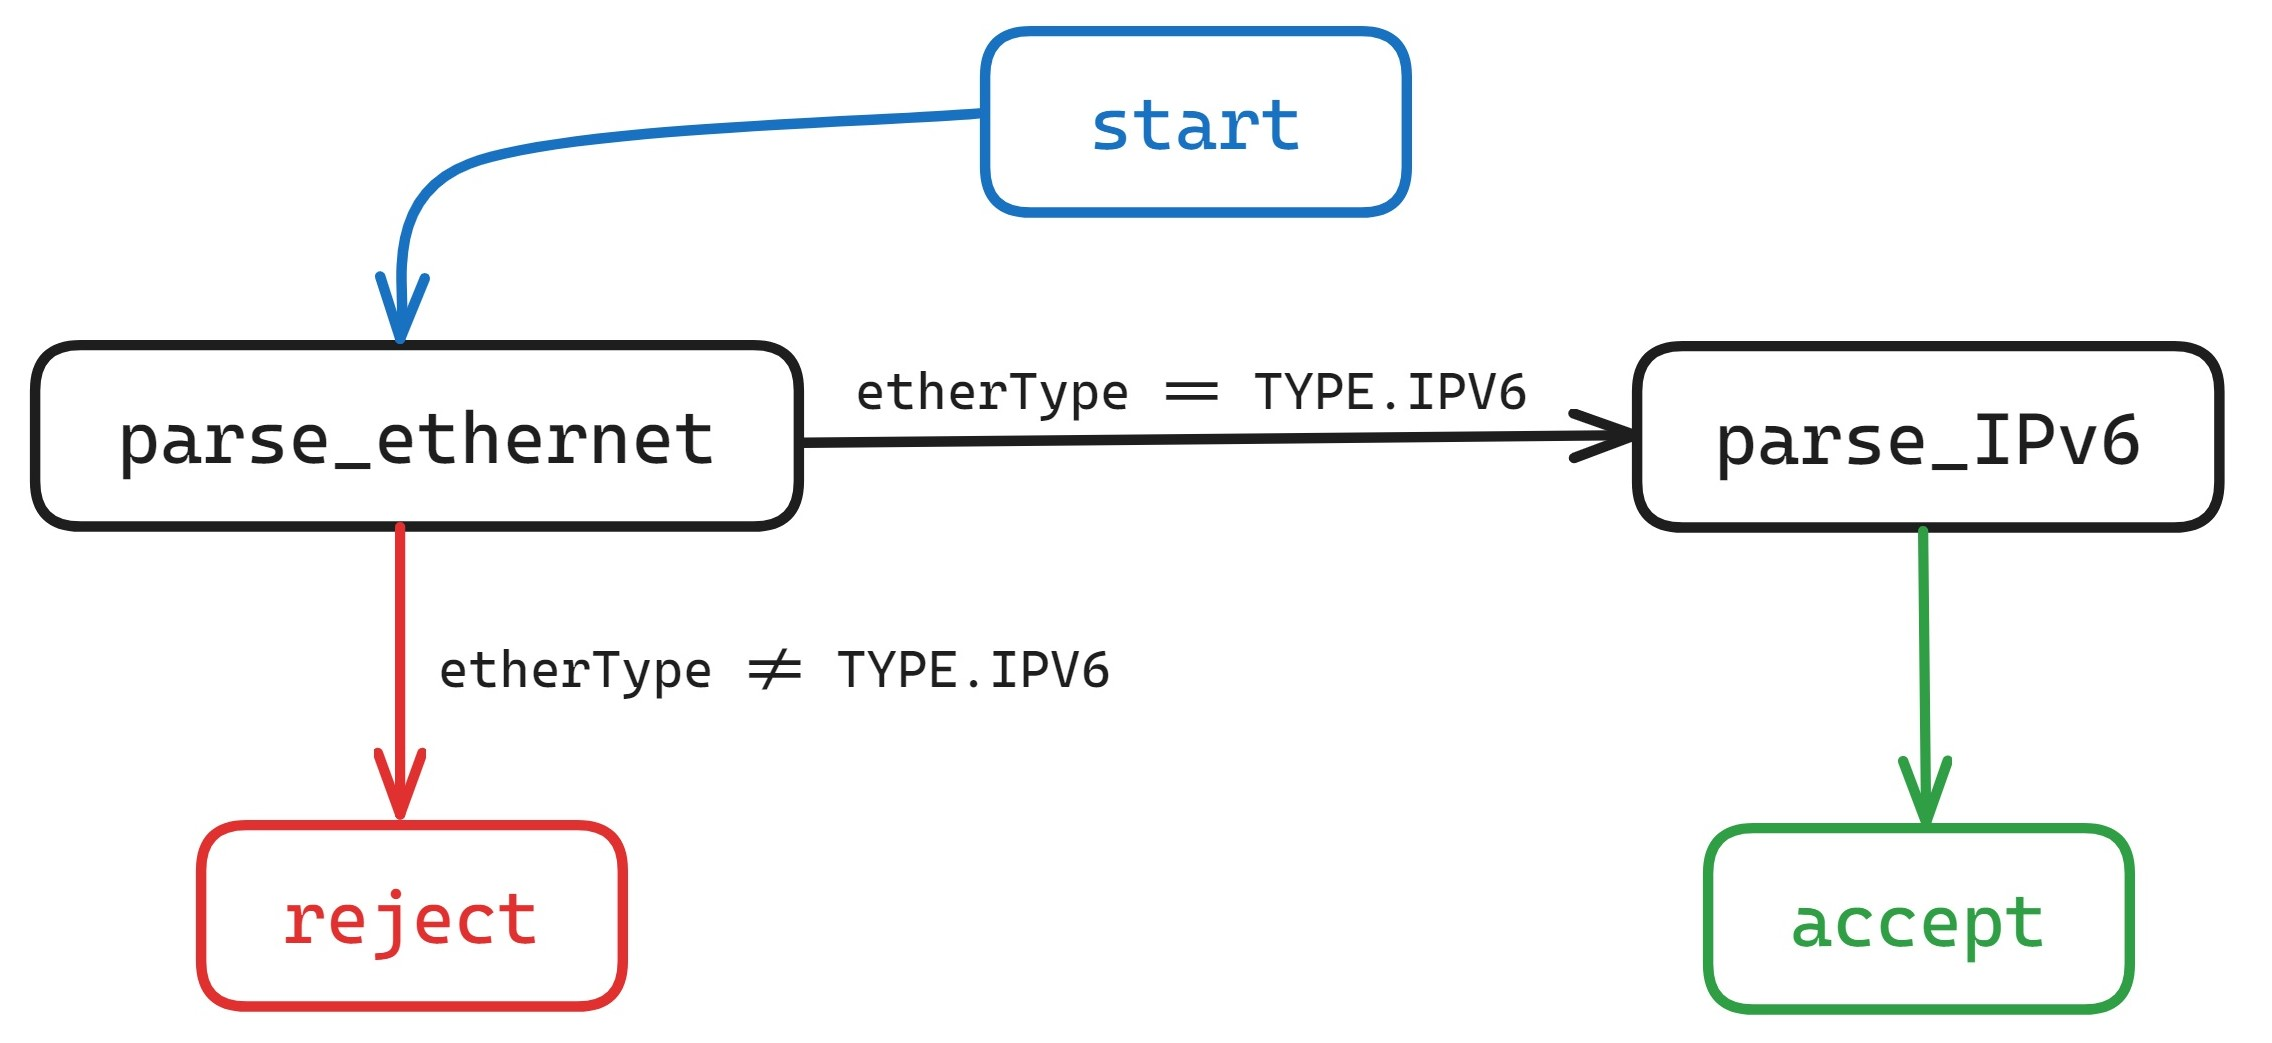
\includegraphics[width=0.6\textwidth]{figures/implementation/ipv6_parser.jpg}
     \caption{IPv6 forwarding parser state machine diagram.}
     \label{fig:impl-ipv6parser}
\end{figure}

\textbf{Checksum Verification} ~ IPv6 does not use checksums, so this pipeline stage is unused, and the code block is left empty.

\textbf{Ingress Processing} ~ Since we only have IPv6 forwarding, the control flow is relatively simple. It is illustrated in \cref{fig:impl-ipv6apply}, where a packet will either be forwarded or dropped, based on its header fields and the data plane's table entries. If the Hop Limit is larger than one, a longest prefix match is performed on the destination address of the packet. If a match is found, the IPv6 forward action is called, which assigns an output port, updates the Ethernet’s source and destination addresses based on the next hop to be taken, and decrements the IPv6 Hop Limit field. A code snippet of the IPv6 forwarding action can be seen in \cref{fig:impl-ipv6forward}.

\begin{figure}[htbp]
  \centering
    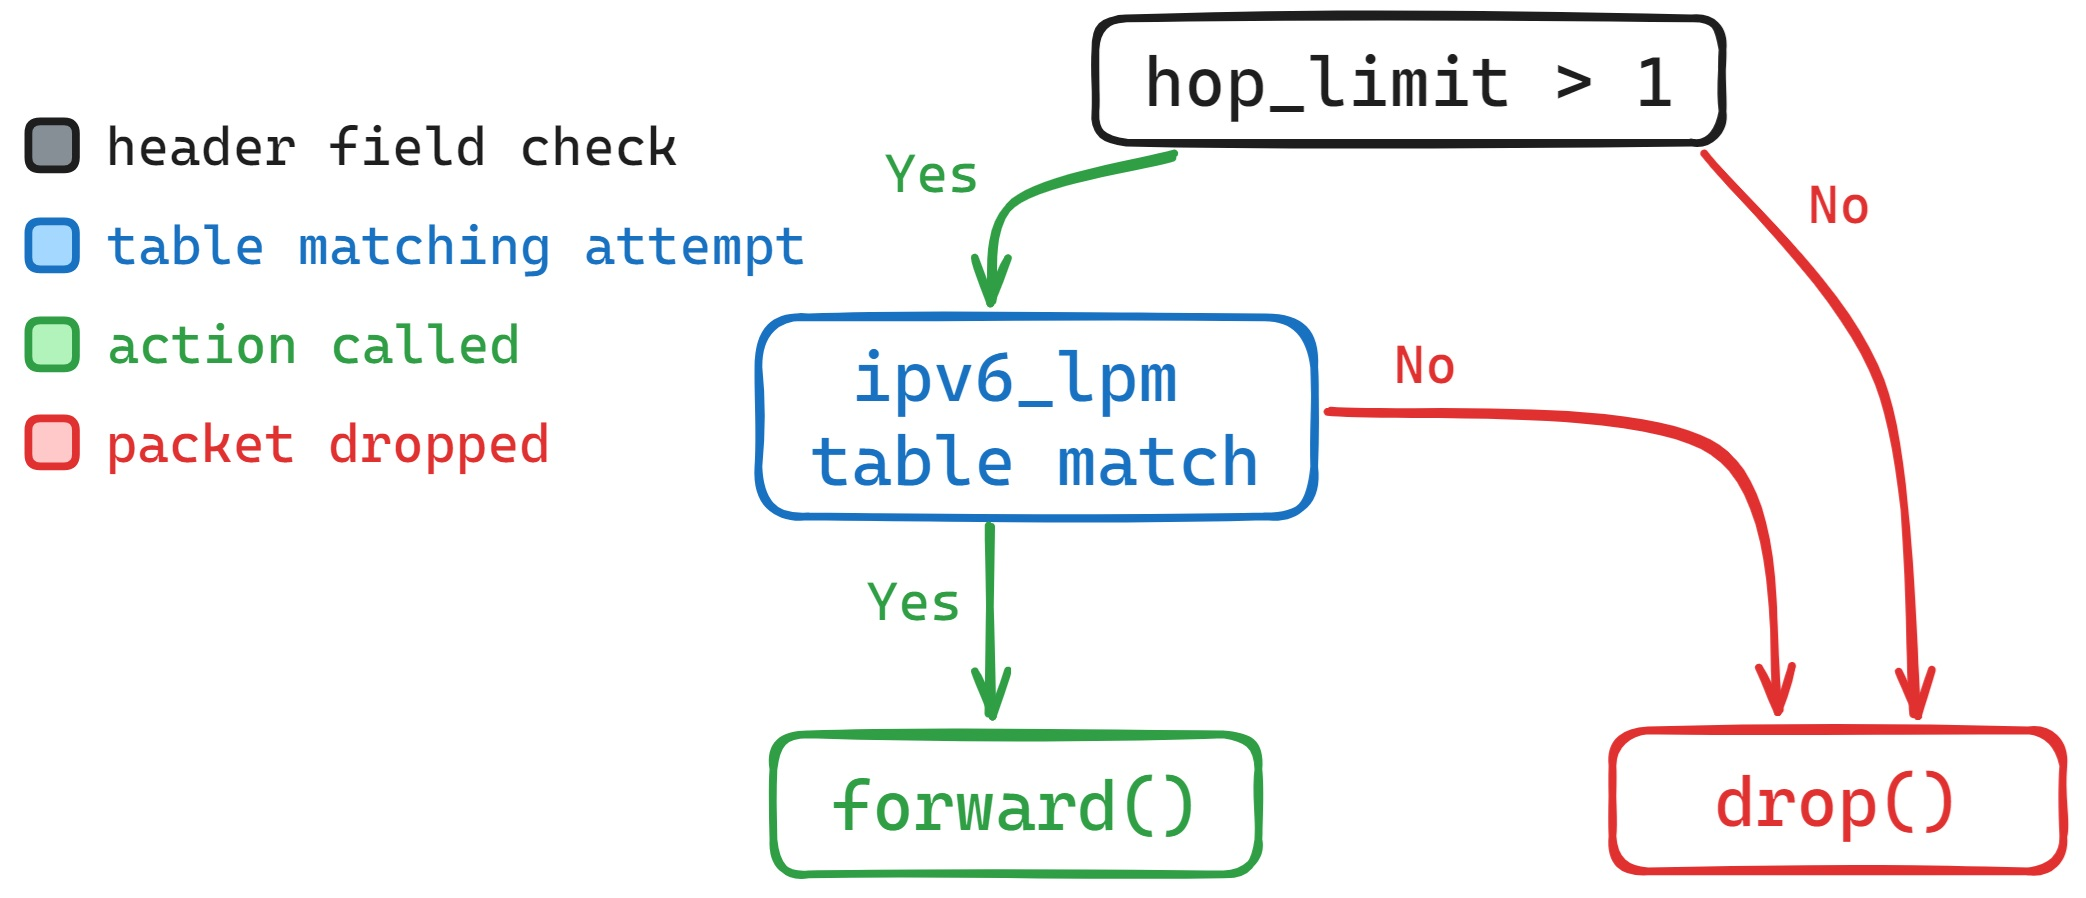
\includegraphics[width=0.6\textwidth]{figures/implementation/ipv6_apply.jpg}
     \caption{IPv6 forwarding control flow represented as a simplified decision tree.}
     \label{fig:impl-ipv6apply}
\end{figure}

\begin{figure}[htbp]
  \centering
    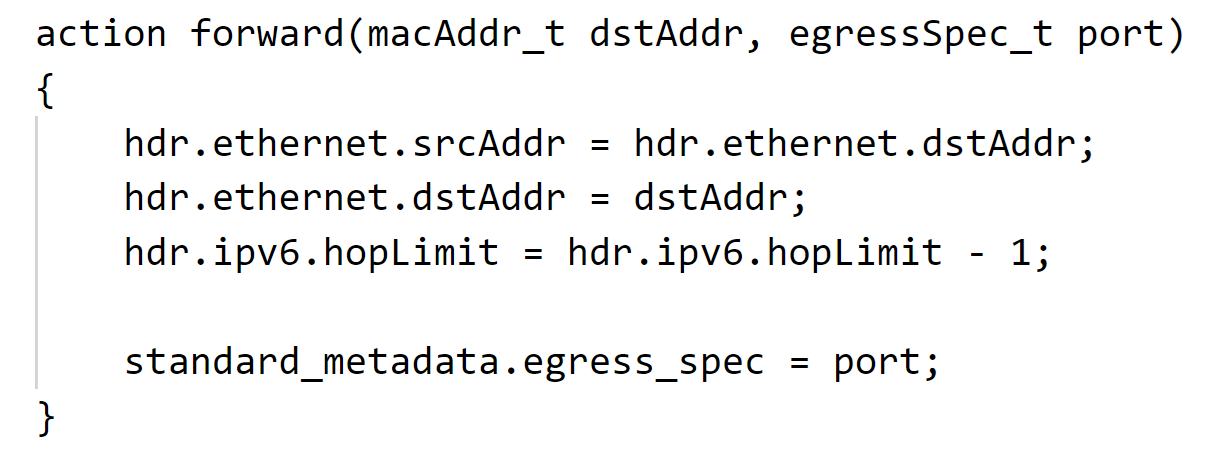
\includegraphics[width=0.6\textwidth]{figures/implementation/ipv6_forward.png}
     \caption{IPv6 forwarding action code block.}
     \label{fig:impl-ipv6forward}
\end{figure}

\textbf{Checksum Calculation} ~ Once again, this pipeline stage is unused.

\textbf{Deparser} ~ The payload proceeds to the deparser stage, where the updated headers are prepended before it is sent out of the router through the assigned egress port.

This program provides functionalities required for parsing, table matching, and forwarding IPv6 packets from one subnet to another. The two hosts are able to discover each other on the network and exchange packets. This fulfils my project's core objectives.


\section{ICMPv6 (Internet Control Message Protocol)}
\label{sec:3.5}

The first extension in my project is to implement ICMPv6 functionalities. ICMPv6 is used to report network errors and provide diagnostic functions. To demonstrate that core ICMPv6 functionalities work, I implement four of the most common messages. Specifically, I implement two informational messages (Echo Request/Reply) and two error messages (Destination Unreachable and Time Exceeded). 



\subsection{ICMPv6 Packet Formats}
\label{sec:3.5.1}

ICMPv6 packets are encapsulated in an IPv6 payload. They all have Type, Code and Checksum fields, but the rest of the packet differs depending on the specific message being relayed. Even though IPv6 does not have checksums, ICMPv6 does. ICMPv6 checksums are calculated using an IPv6 pseudoheader \cite{ICMPv6Specs}. The Echo Reply and Echo Response packets have optional data such as a timestamp, and the error messages have a payload containing the first bytes of the original packet that triggered the error. The formats of the Echo Request/Reply, Time Exceeded packets, and Destination Unreachable are shown in \cref{fig:impl-echoheader}, \cref{fig:impl-timeexheader}, and \cref{fig:impl-destunrheader}, respectively.

\begin{figure}[htbp]
\begin{subfigure}{\textwidth}
  \centering
  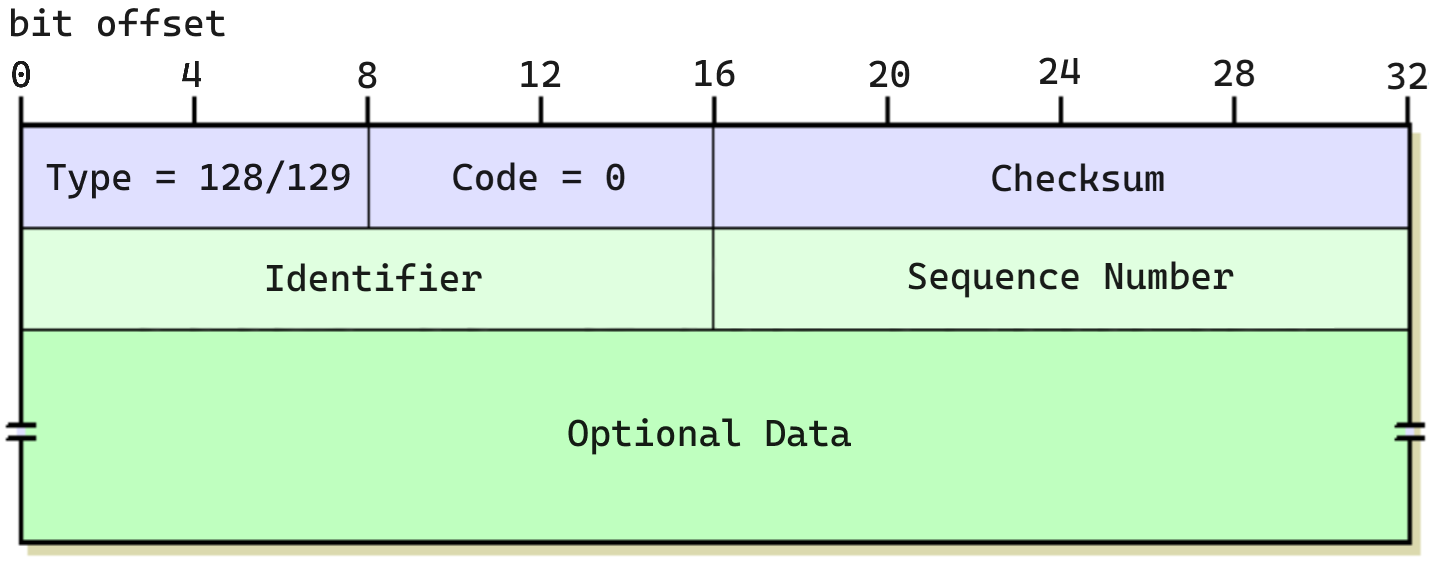
\includegraphics[width=0.5\textwidth]{figures/implementation/icmpv6_echo.png}
  \caption{Echo Request/Reply.}
  \label{fig:impl-echoheader}
\end{subfigure}
\par \medskip
\begin{subfigure}{.5\textwidth}
  \centering
  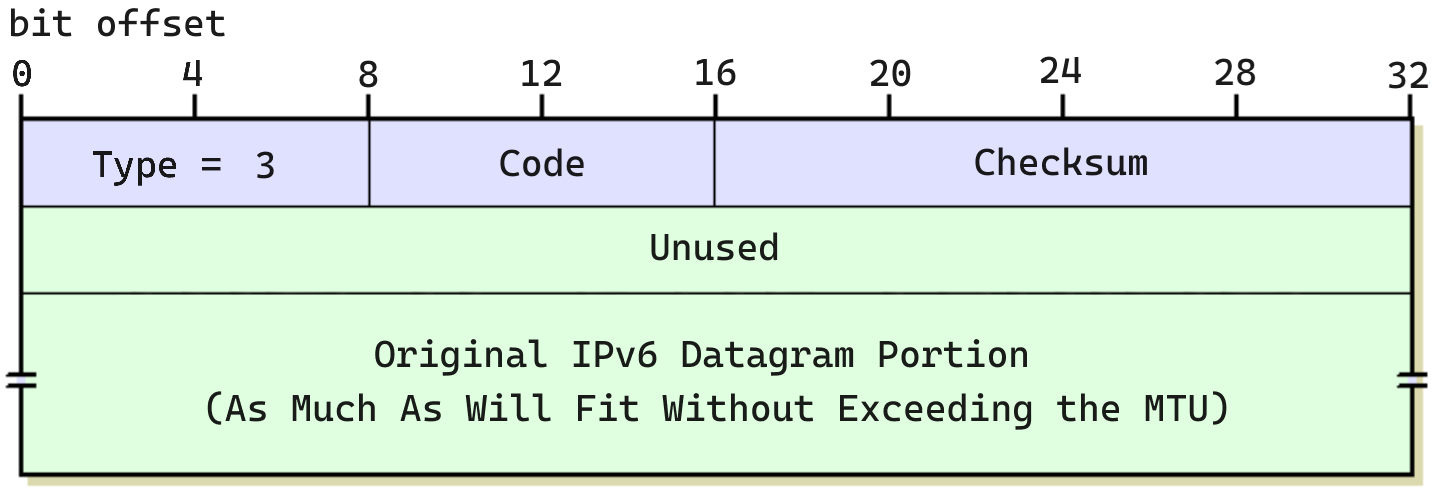
\includegraphics[width=1\textwidth]{figures/implementation/icmpv6_timeexceeded.png}
  \caption{Time Exceeded.}
  \label{fig:impl-timeexheader}
\end{subfigure}%
\begin{subfigure}{.5\textwidth}
  \centering
  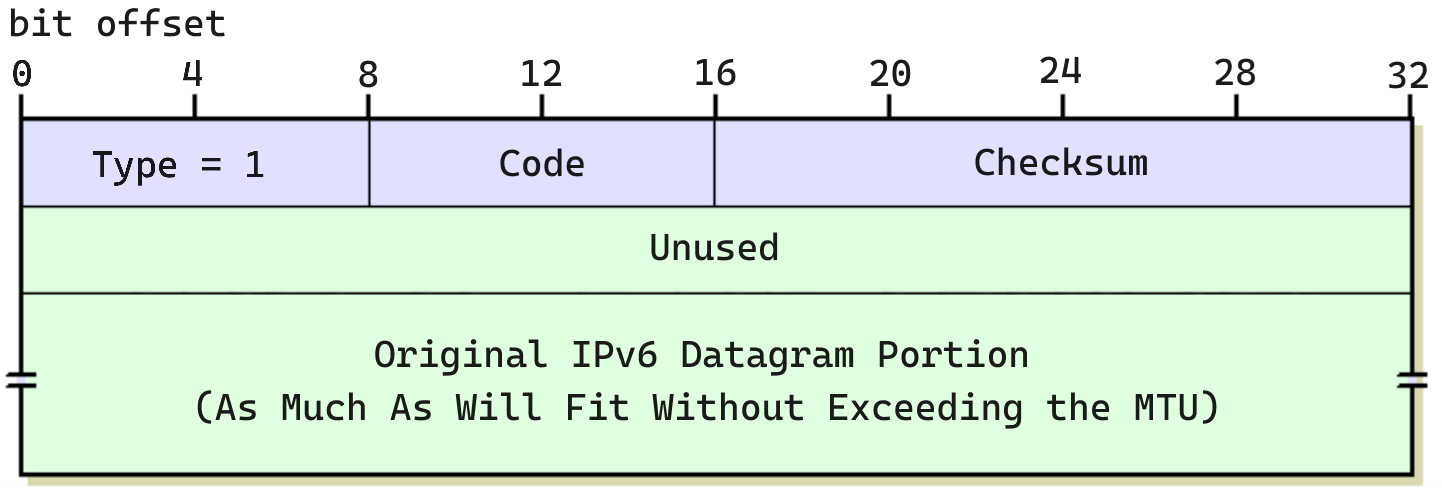
\includegraphics[width=1\textwidth]{figures/implementation/icmpv6_destunreachable.png}
  \caption{Destination Unreachable.}
  \label{fig:impl-destunrheader}
\end{subfigure}
\caption{ICMPv6 packet formats. Adapted from \cite{IPguide}.}
\label{fig:test}
\end{figure}


\subsection{ICMPv6 Design}
\label{sec:3.5.2}

An Echo Request directed at a defined router address receives an Echo Reply. A Destination Unreachable error message is generated if the destination address of the Echo Request is unknown to the router, and a Time Exceeded error message is generated if the Echo Request reaches the router with a remaining Hop Limit of zero or one. For more detailed information on how to run this experiment, consult Appendix D.

I design the program such that it can trivially be extended to support other ICMPv6 messages. For example, a packet with a malformed header would not pass a header validity test in the program. If that happens, the current design of the router would drop the packet. Instead, a new action could be defined to return a Parameter Problem error message.



\subsection{ICMPv6 Program}
\label{sec:3.5.3}

The data plane behaviour of the router is defined by the P4 file \texttt{icmpv6.p4}.

\textbf{Header Definitions} ~ I define two additional header types: a 4-byte ICMPv6 header, which contains Type, Code, and Checksum fields; and a 60-byte Echo header, which contains Identifier and Sequence Number fields, and a payload for the optional data.

\textbf{Parser} ~ The parser state machine of this program reflects the addition of the ICMPv6 and Echo headers and only accepts packets that are Echo Requests. It identifies these packets by checking the Next Header field in the extracted IPv6 header, and the Type field of the ICMPv6 header. The parser state machine diagram is shown in \cref{fig:impl-icmpv6parser}.

\begin{figure}[htbp]
  \centering
    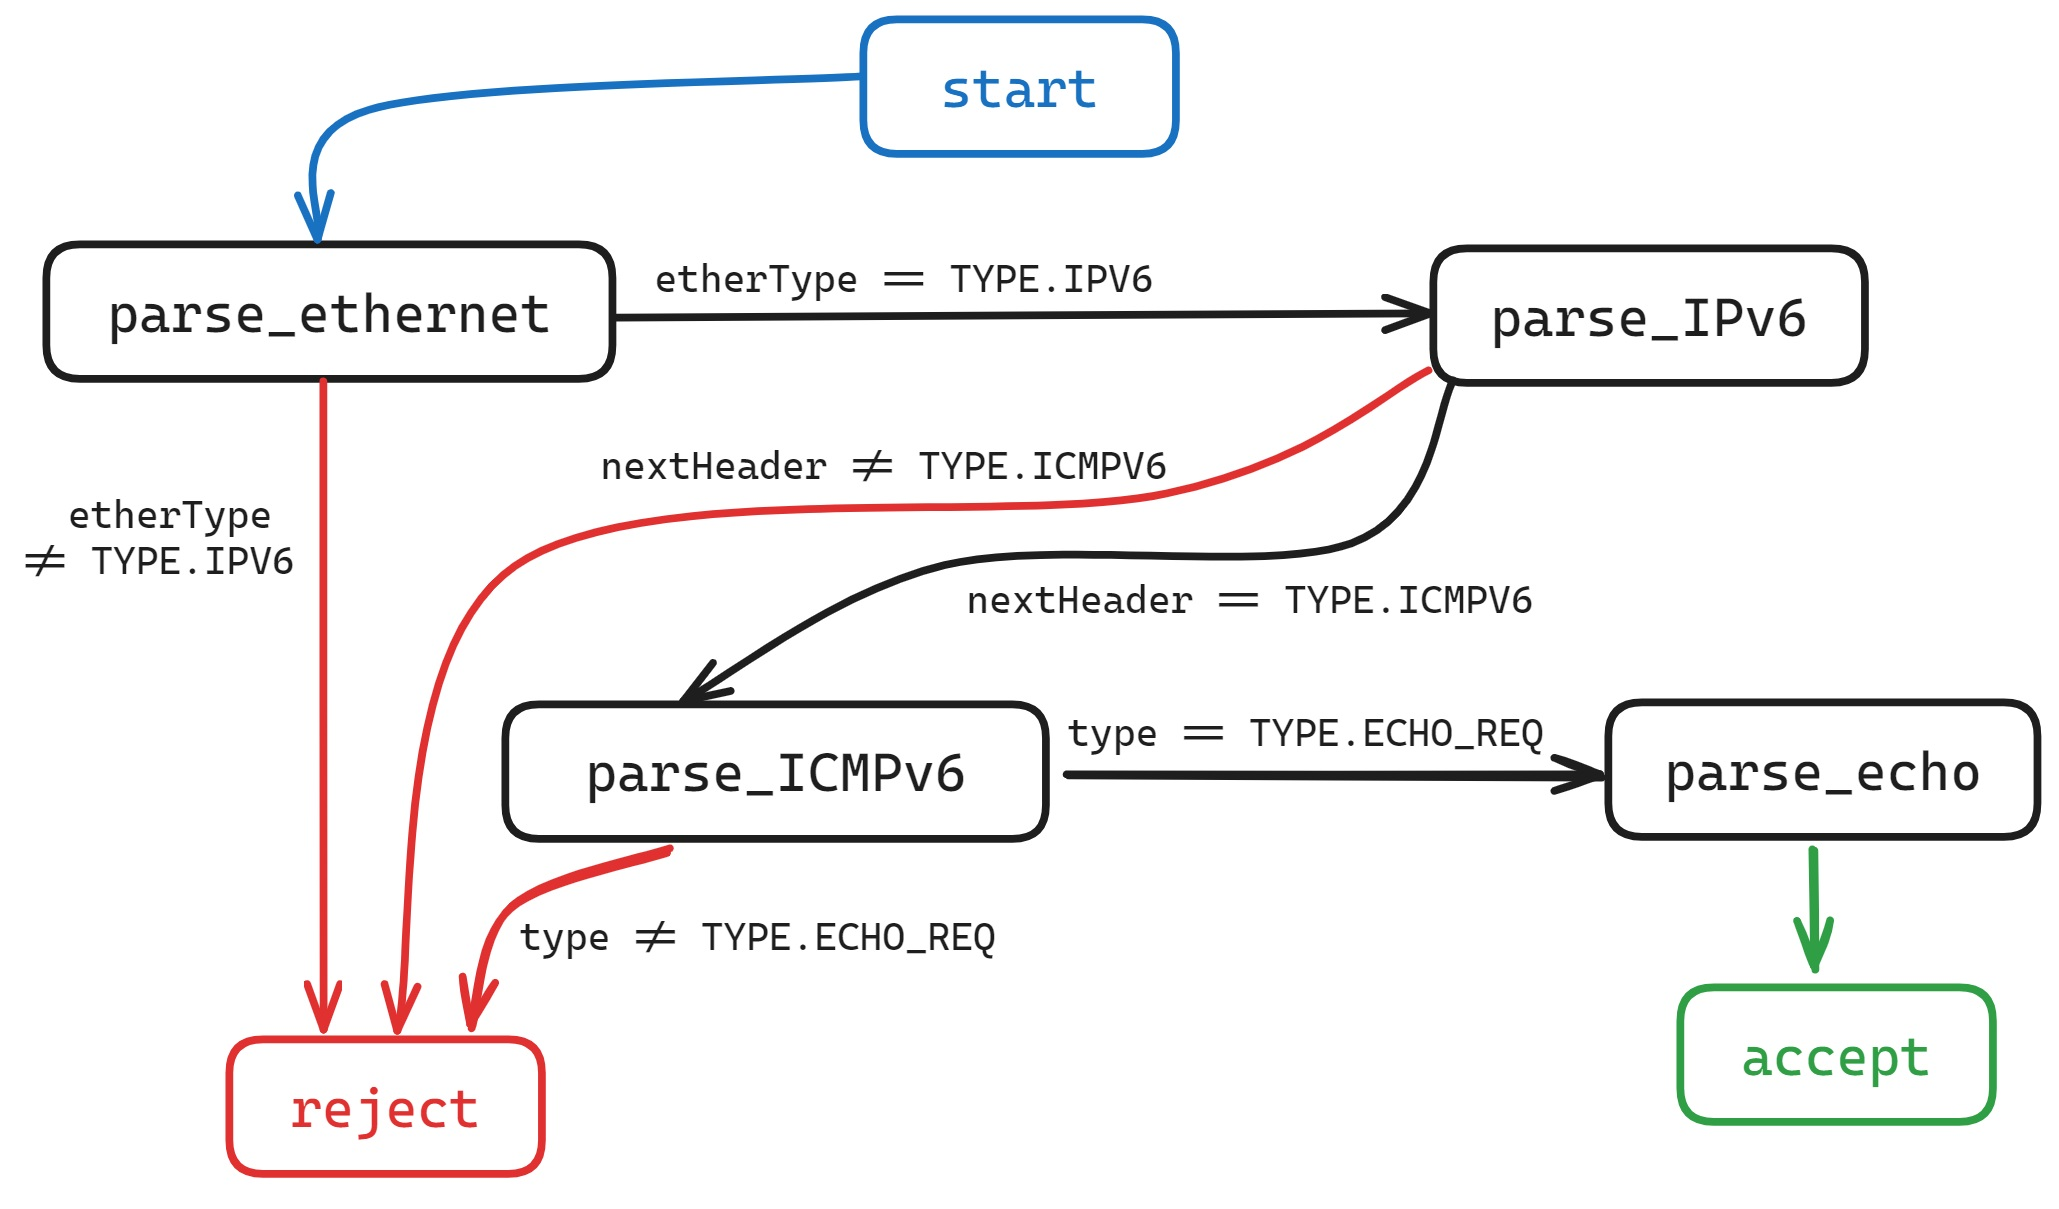
\includegraphics[width=0.70\textwidth]{figures/implementation/icmpv6_parser.jpg}
     \caption{ICMPv6 parser state machine diagram.}
     \label{fig:impl-icmpv6parser}
\end{figure}

\textbf{Checksum Verification} ~ The ICMPv6 checksum is verified before the packet proceeds to ingress control blocks. ICMPv6 checksums are calculated using all fields in the ICMPv6 packet, along with an IPv6 pseudoheader, made up of the source and destination addresses, the payload length, and the Next Header field value. The checksum function splits the data into 16-bit pieces and one's complement sums all of them by carrying the one if the sum overflows. The checksum is then the 16 bit one's complement of the result.

\textbf{Ingress Processing} ~ The first performed check is on the Hop Limit -- if it is less than or equal to one, the Time Exceeded action is called. If it is larger than one, the next check is on the ICMPv6 Type field. Even though this program's parser only accepts packets of type Echo Request, I added this redundant check for easier integration into the IPv6 router. If the packet is of type Echo Request, the destination address is checked in the Echo Responder table, otherwise it is dropped. The Echo Responder table matches the address to its statically defined entries (the router’s addresses) in the P4 program. If a match is found in the table, the Echo Reply action is called, otherwise the Destination Unreachable action is triggered. For both error messages, a longest prefix match table is used to identify which subnet the packet came from in order to send the error message from the respective router IPv6 address and towards the respective subnet’s port. The control flow of the ingress block is shown in \cref{fig:impl-icmpv6apply}.

\begin{figure}[htbp]
  \centering
    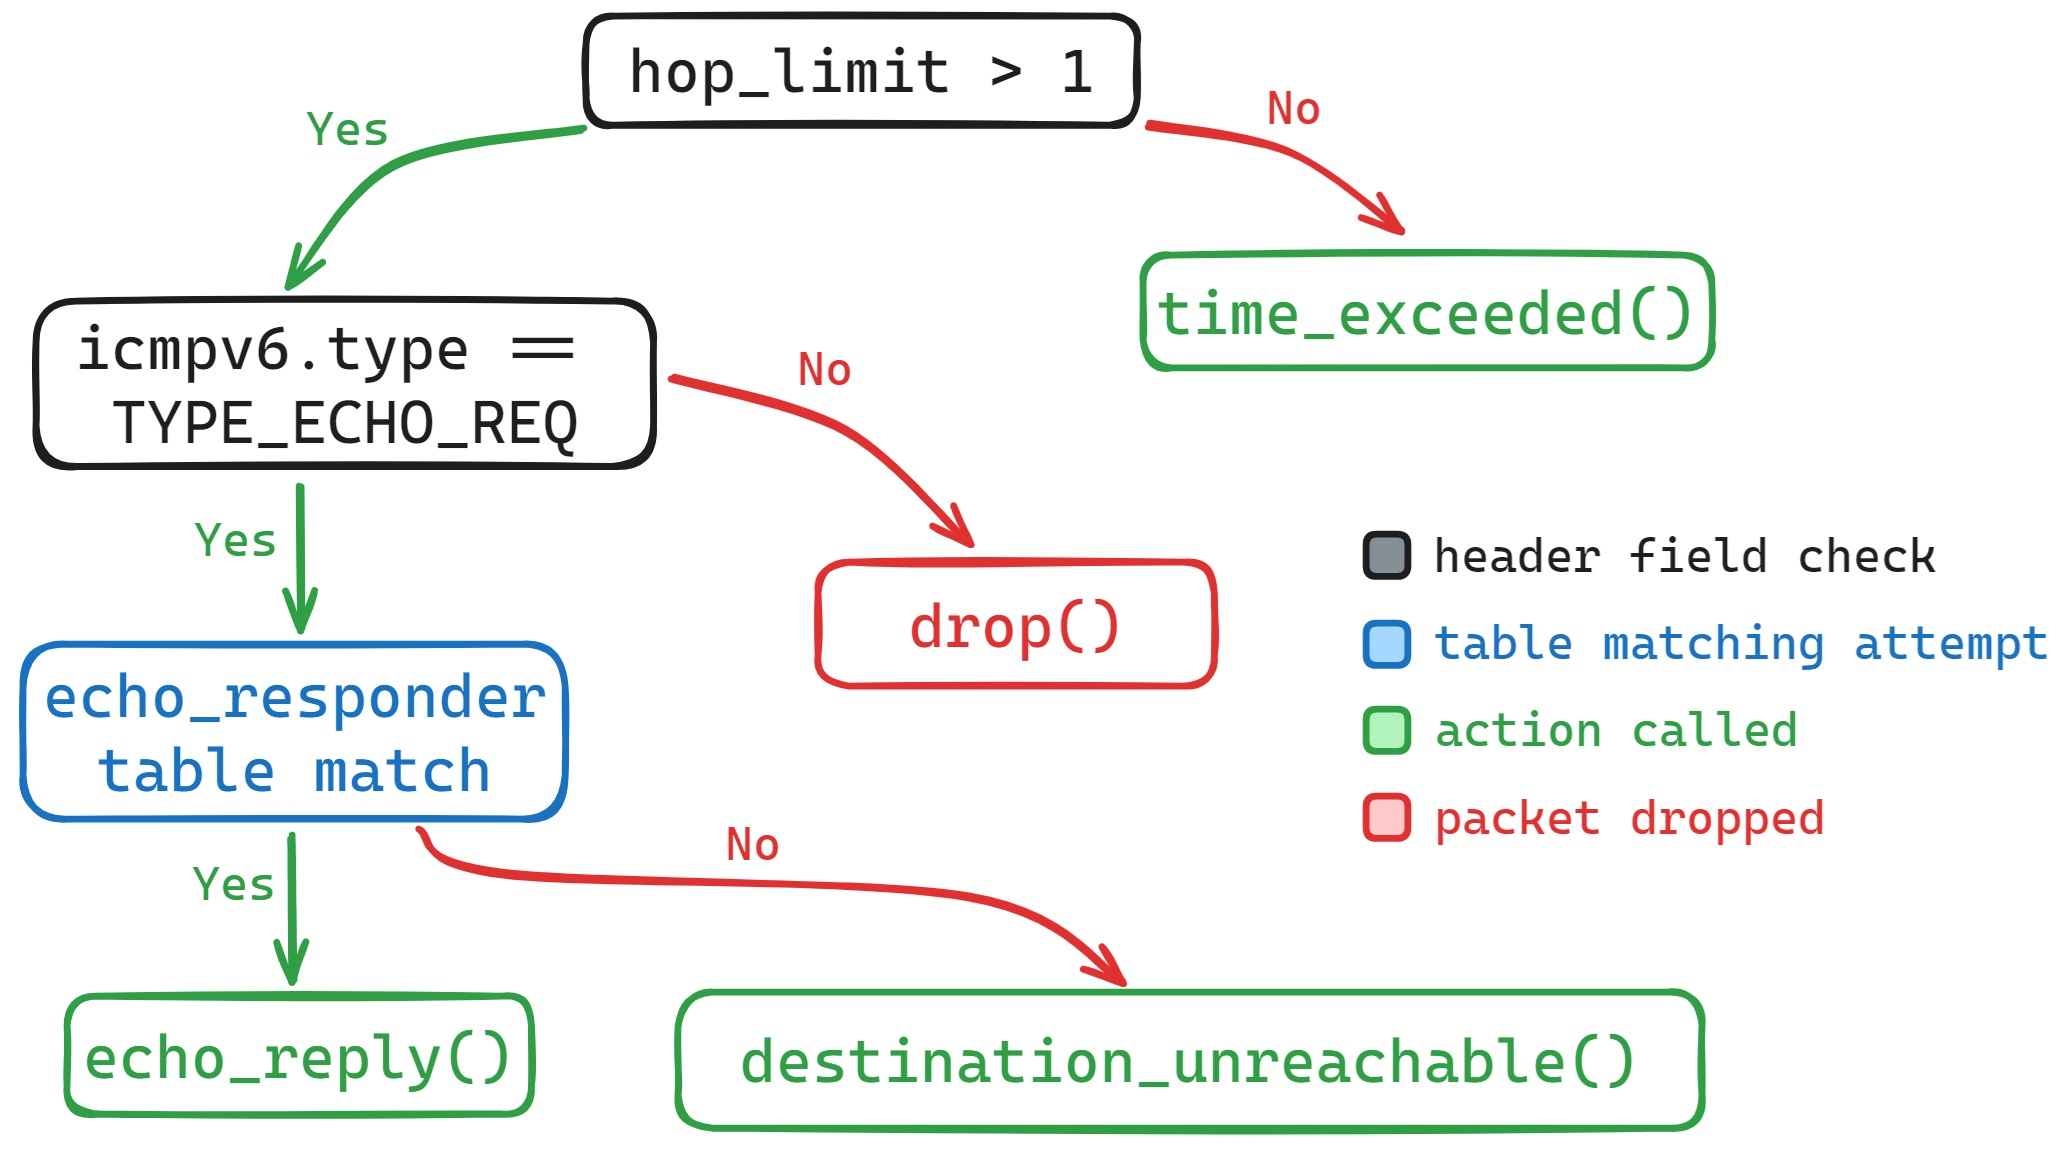
\includegraphics[width=0.65\textwidth]{figures/implementation/icmpv6_apply.jpg}
     \caption{ICMPv6 control flow represented as a simplified decision tree.}
     \label{fig:impl-icmpv6apply}
\end{figure}

When an action is called, the Type field of the ICMPv6 packet is updated accordingly. For an Echo Response no other ICMPv6 fields are modified. For generating error messages, the packet payload is updated to the original packet's dataframe. In all cases, the source addresses of the IPv6 and Ethernet headers are updated to match the corresponding subnet’s router addresses and the destination addresses are set to the original packet’s source addresses. The code block for the Echo Reply action is shown in \cref{fig:impl-icmpv6echoreply}.

\begin{figure}[htbp]
  \centering
    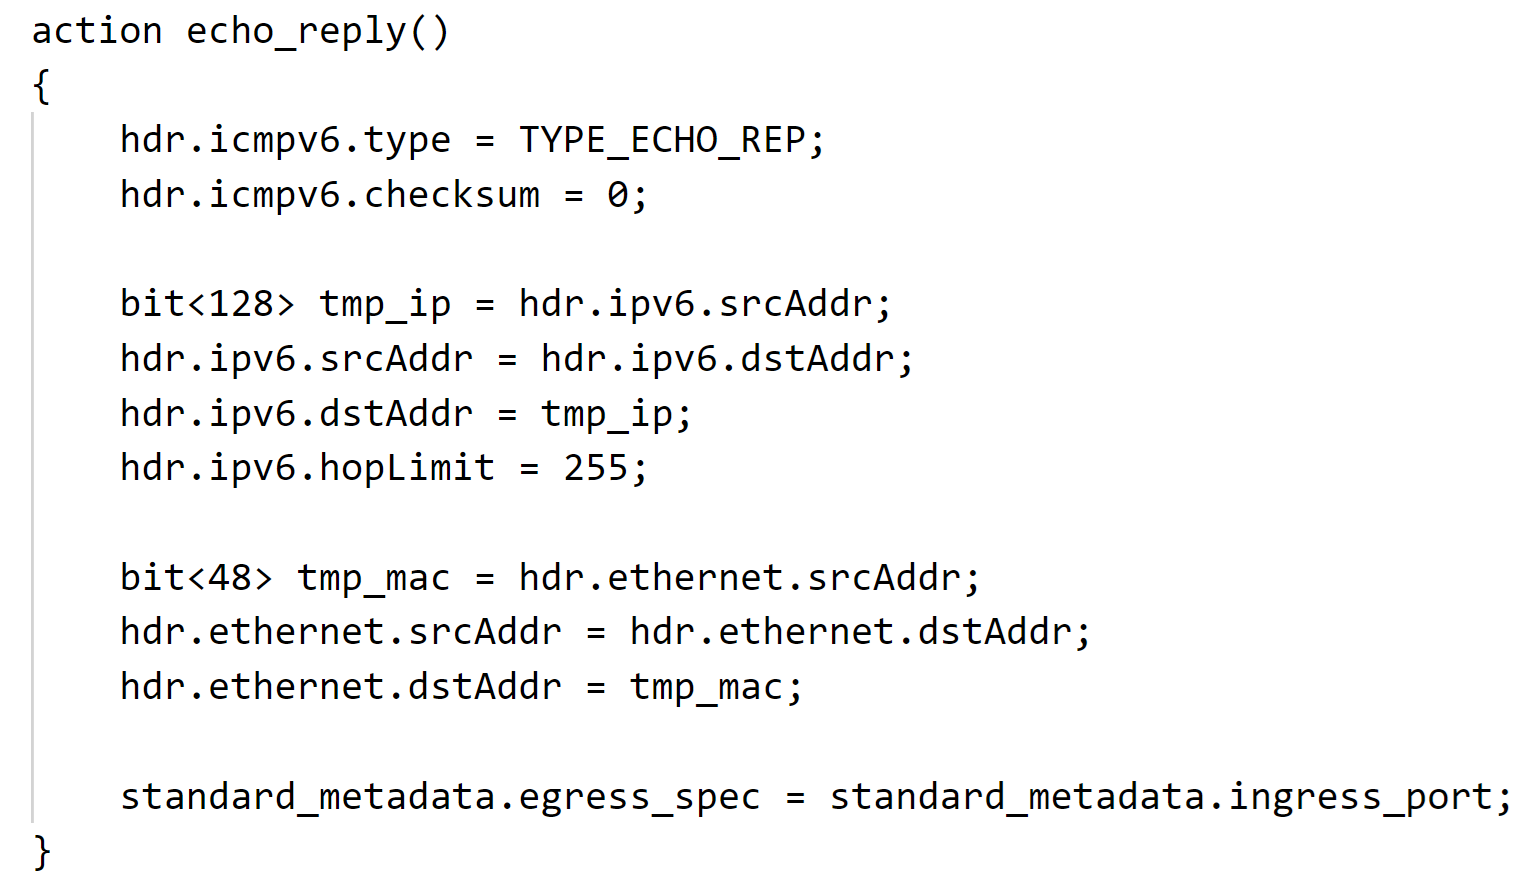
\includegraphics[width=0.7\textwidth]{figures/implementation/icmpv6_echoreply.png}
     \caption{ICMPv6 Echo Reply action code block.}
     \label{fig:impl-icmpv6echoreply}
\end{figure}

\textbf{Checksum Calculation} ~ An ICMPv6 checksum computation is performed using an IPv6 pseudoheader, and the value is placed in the ICMPv6 Checksum field.

\textbf{Deparser} ~ The deparser prepends all headers onto the outgoing packet before sending it out of the specified egress port into the correct subnet.

This program implements core ICMPv6 functionalities and allows for the code to be extended to support other ICMPv6 messages. A host that sends an Echo Request to the router receives an Echo Reply. Any packet that has exceeded the Hop Limit generates a Time Exceeded error message from the router, and any packet whose destination address is not known to the router generates a Destination Unreachable error message. This concludes my first project extension. 



\section{NDP (Neighbour Discovery Protocol)}
\label{sec:3.6}

My second project extension is to implement NDP functionalities. Nodes use NDP to learn about network configurations and nodes' link-layer addresses. In IPv6, Neighbour Discovery happens on top of the network layer, using ICMPv6 messages. There are five different packet types in ICMPv6 that are used for NDP purposes, and I implement two of them -- Neighbour Solicitation (NS) and Neighbour Advertisement (NA) -- to show that my router can support NDP functionalities.



\subsection{NDP Packet Formats}
\label{sec:3.6.1}

NS and NA packets start as all ICMPv6 packets do: with Type, Code and Checksum fields. The remainder of the packet contains 32 reserved bits (three bits of which are used for flags in the NA packet) and the address that needs to be resolved. The NA packet puts the link-layer address of the target IPv6 address in the options field. All NDP packets are encapsulated within an IPv6 payload. NS and NA packet formats can be seen in \cref{fig:impl-ndpsolheader} and \cref{fig:impl-ndpadvheader}, respectively.

\begin{figure}[htbp]
\centering
\begin{subfigure}{.5\textwidth}
  \centering
  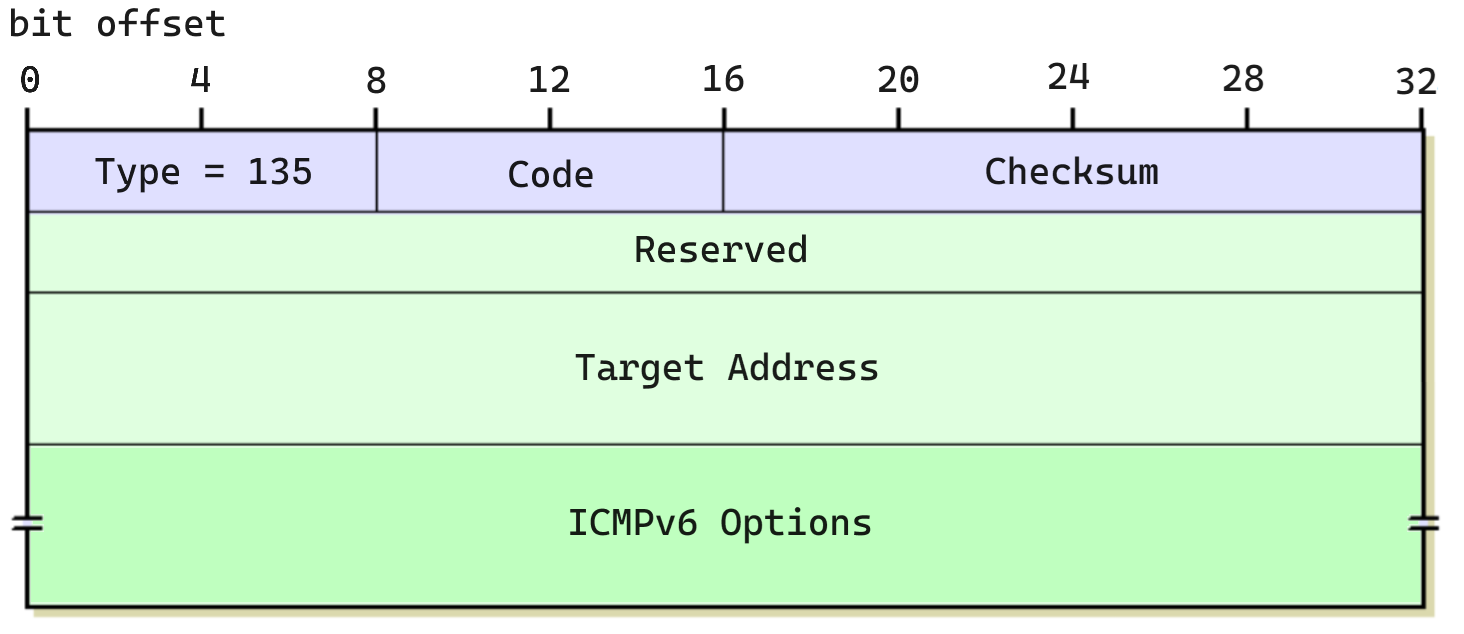
\includegraphics[width=1\linewidth]{figures/implementation/ndp_sol.png}
  \caption{Neighbour Solicitation packet format.}
  \label{fig:impl-ndpsolheader}
\end{subfigure}%
\begin{subfigure}{.5\textwidth}
  \centering
  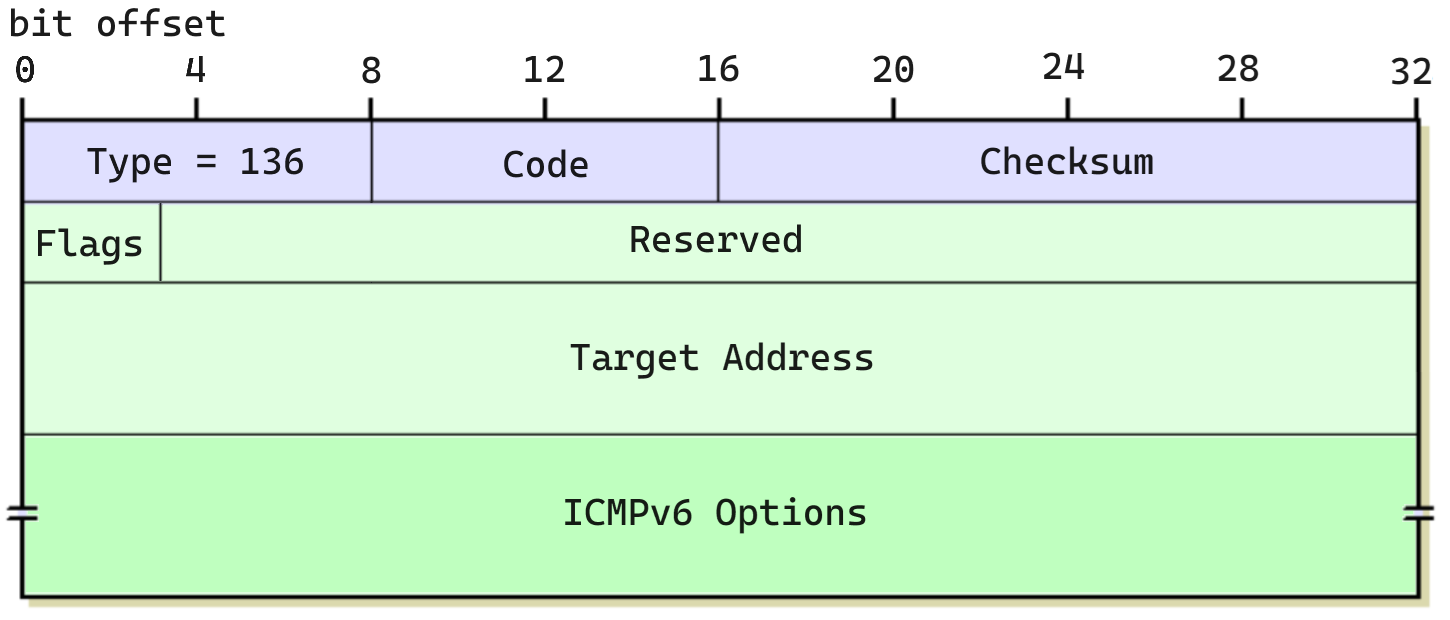
\includegraphics[width=1\linewidth]{figures/implementation/ndp_adv.png}
  \caption{Neighbour Advertisement packet format.}
  \label{fig:impl-ndpadvheader}
\end{subfigure}
\caption{NDP packet formats. Adapted from \cite{IPguide}.}
\label{fig:impl-ndpmsgs}
\end{figure}



\subsection{NDP Design}
\label{sec:3.6.2}

The router's tables are populated with IPv6-MAC address pairs using the CLI. The router responds to any NS whose target address it recognises with an NA that contains the corresponding link-layer address. Since NDP acquires next-hop MAC addresses, I do not manually input any neighbour entries into the hosts, unlike in previous experiments. Issuing Echo Requests results in the hosts’ neighbour tables populating the entries they receive from the router. Appendix E contains details on how to run this experiment. Once again, I design the program in a way that allows for it to trivially be extended to support other NDP messages.



\subsection{NDP Program}
\label{sec:3.6.3}

The data plane behaviour of the router is defined by the P4 file \texttt{ndp.p4}.

\textbf{Header Definitons} ~ I define a new header type in place of the Echo header: a 28-byte Nei header, containing 3 bit flags, reserved bits, a target address, an Options Type field, an Options Length field, and a payload.

\textbf{Parser} ~ The parser state machine of this program, seen in \cref{fig:impl-ndpparser}, is similar to the one in extension 1, \cref{fig:impl-icmpv6parser}, with the \texttt{Echo} state being replaced by the \texttt{Nei} state. Only packets of type NS are accepted by the parser.

\begin{figure}[htbp]
  \centering
    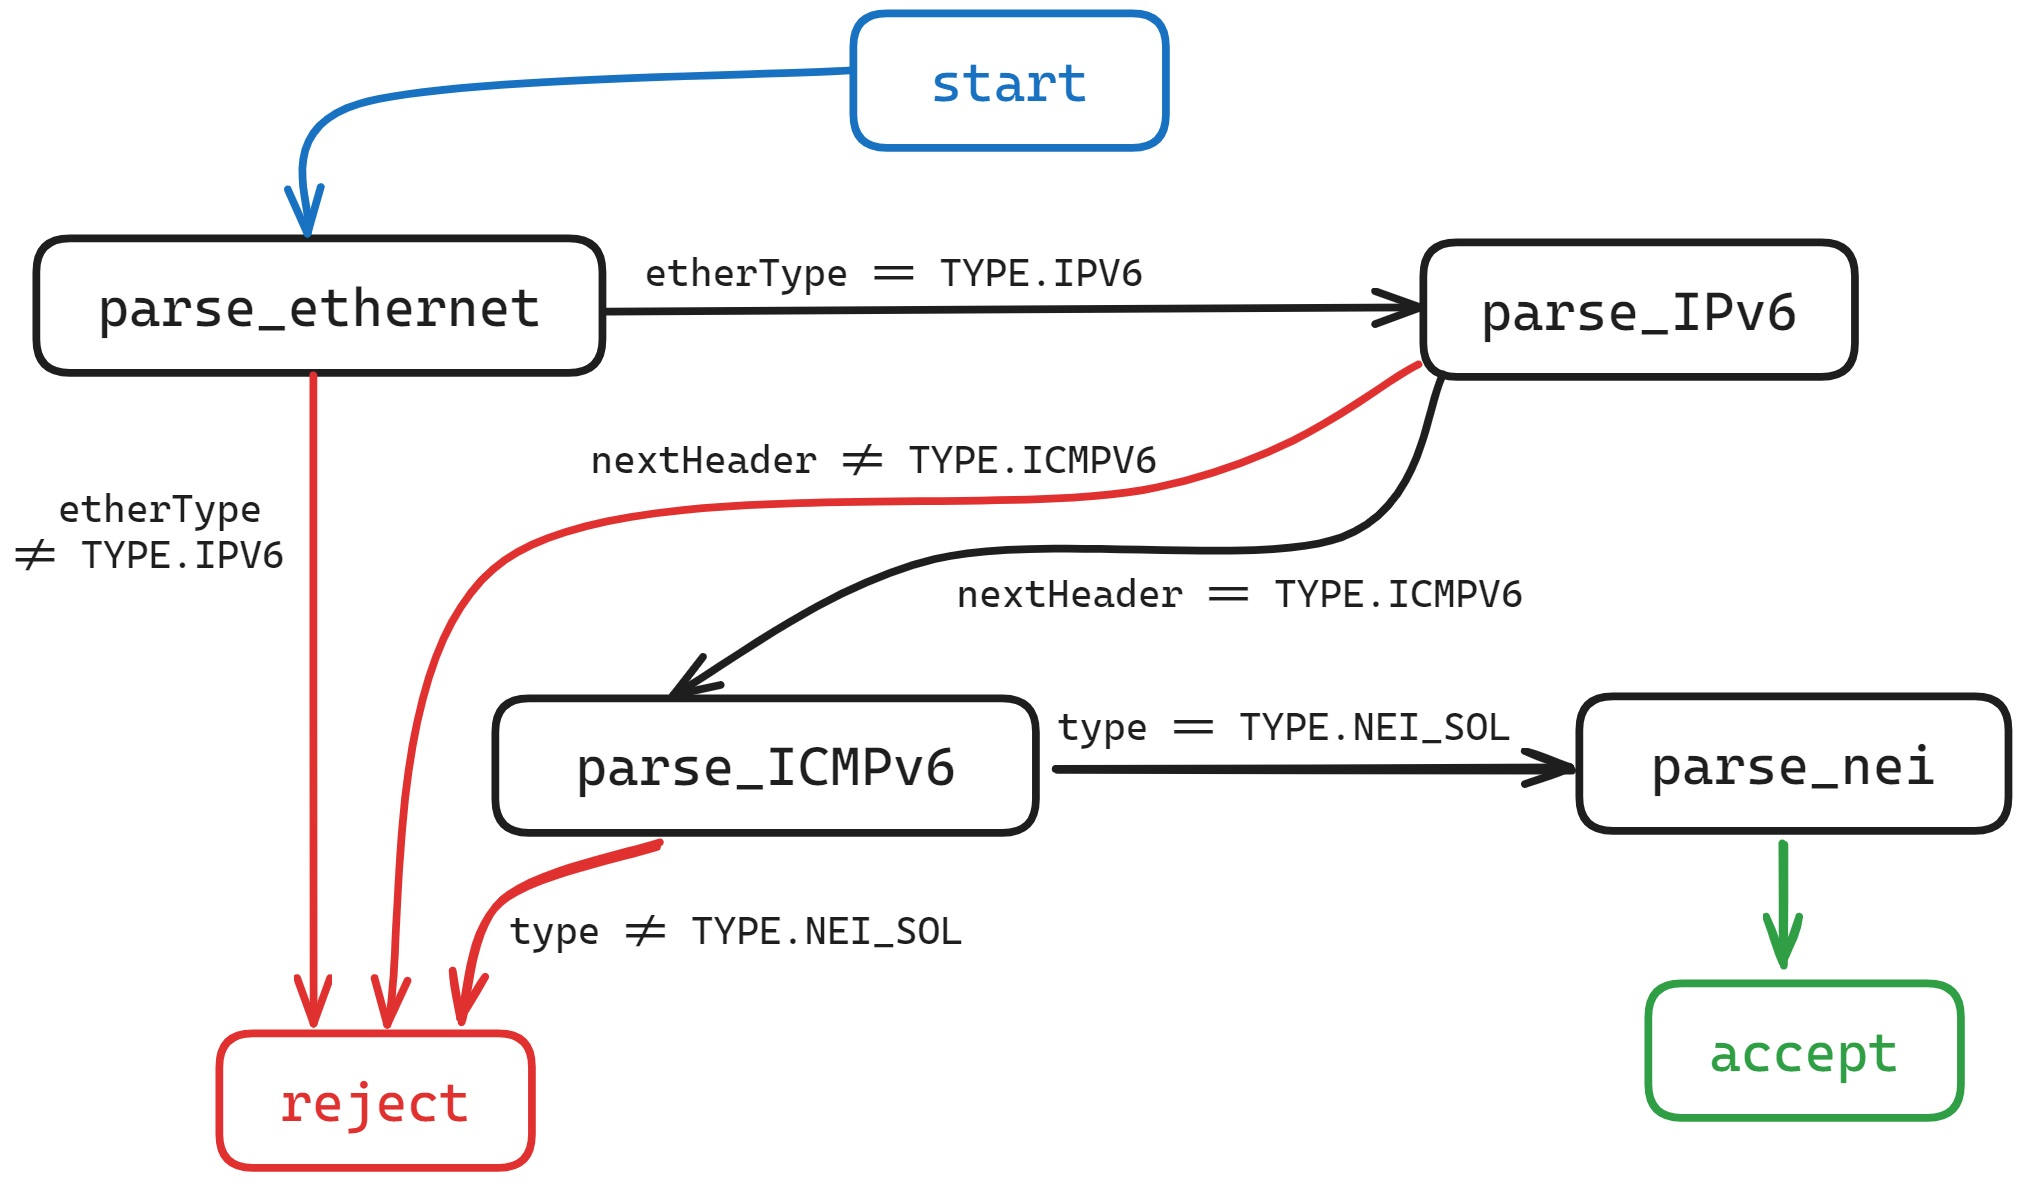
\includegraphics[width=0.60\textwidth]{figures/implementation/ndp_parser.jpg}
     \caption{NDP parser state machine diagram.}
     \label{fig:impl-ndpparser}
\end{figure}

\textbf{Checksum Verification} ~ The ICMPv6 checksum is calculated and verified.

\textbf{Ingress Processing} ~ The router only generates a response if the Hop Limit has not expired, the packet is of type NS, and there is a hit for the target address in the Neighbour Responder table. The control flow for ingress processing is illustrated in \cref{fig:impl-ndpapply}. The NA action constructs an NA packet that contains the link-layer address of the NS's target IPv6 address. The ICMPv6 Type field and the packet flags are updated, the destination addresses set to the original source addresses, and the source addresses set to the router’s respective subnet address. 

\begin{figure}[htbp]
  \centering
    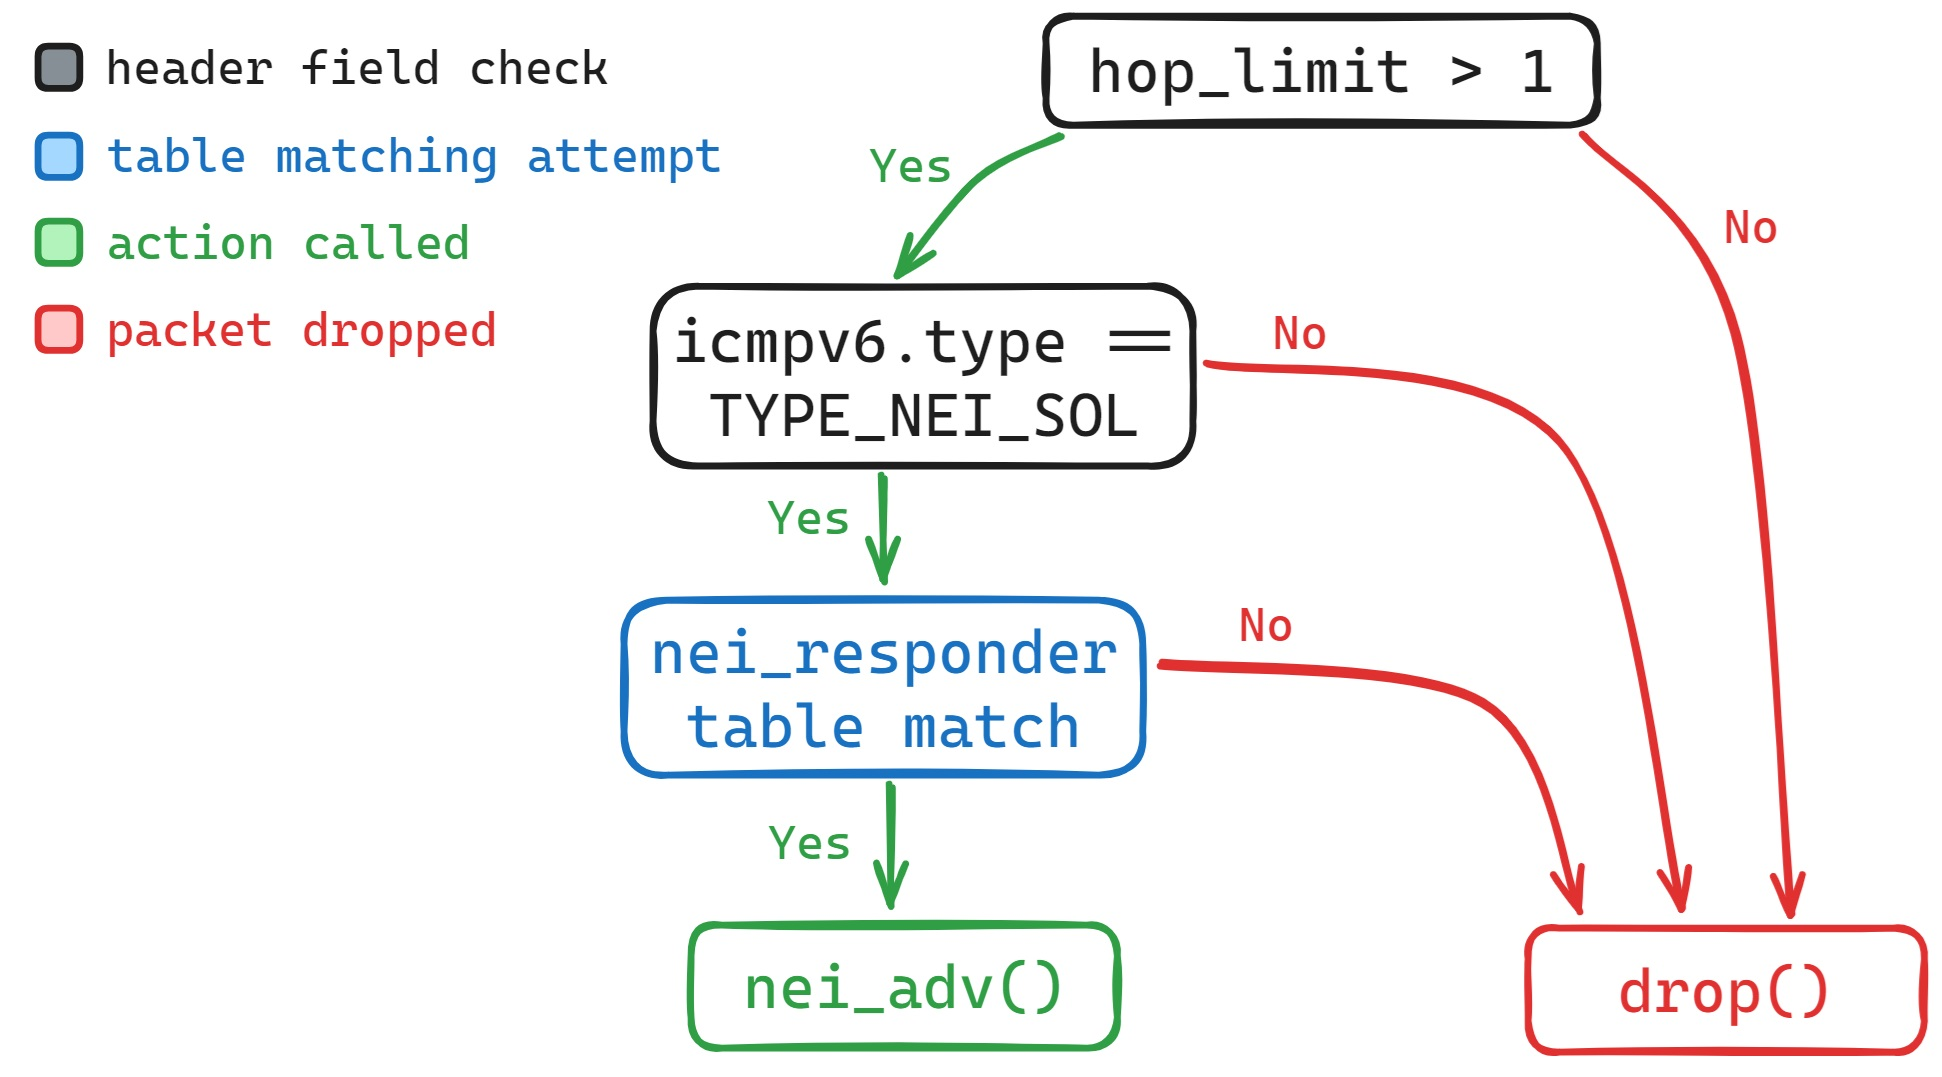
\includegraphics[width=0.65\textwidth]{figures/implementation/ndp_apply.jpg}
     \caption{NDP control flow represented as a simplified decision tree.}
     \label{fig:impl-ndpapply}
\end{figure}

\textbf{Checksum Calculation} ~ The ICMPv6 checksum is calculated and the field updated. 

\textbf{Deparser} ~ The deparser prepends all updated headers and sends the packet to the specified subnet egress port.

This program supports NDP NS and NA functionalities and provides a framework for the implementation to be extended to include other NDP messages. A host sends an NS to the router and receives an NA containing the next-hop MAC address for the target IPv6 address. Hosts can successfully populate their neighbour entry tables through NDP rather than needing manual configuration. This concludes my second project extension.



\section{IPv6 Router}
\label{sec:3.7}

To implement a fully functioning IPv6 router prototype, I combined the functionalities from the three aforementioned sections into one program. My router parses IPv6 packets, checks and updates the Hop Limit, identifies the outbound interface, and forwards the IPv6 packet. Additionally, it responds to Echo Requests and Neighbour Solicitations, and generates Time Exceeded and Destination Unreachable errors, as appropriate.

\subsection{IPv6 Router Design}
\label{sec:3.7.1}

This program supports every functionality outlined in the previous three sections. The code for \texttt{router6.p4} is built by combining the \texttt{ipv6.p4}, \texttt{icmpv6.p4}, and \texttt{ndp.p4} programs. For more detailed information on how to run this experiment, consult Appendix F.

\subsection{IPv6 Router Program}
\label{sec:3.7.2}

The data plane behaviour of the router is defined by the P4 file \texttt{router6.p4}.

\textbf{Header Definitions} ~ All headers defined in \cref{sec:3.4}, \cref{sec:3.5}, and \cref{sec:3.6} are included. A header union is defined to combine the Echo and the Nei headers, as they are both encapsulated within the ICMPv6 payload.

\textbf{Parser} ~ This program's parser merges the respective parsers of the individual functionalities. All intermediate states have been added and additional branches defined when multiple transitions are possible. As before, any packet that is not of type IPv6 gets rejected. Every ICMPv6 packet gets accepted and, if it is identified as an Echo Request or an NS packet, the additional headers also get parsed, as shown in \cref{fig:impl-router6parser}.

\begin{figure}[htbp]
  \centering
    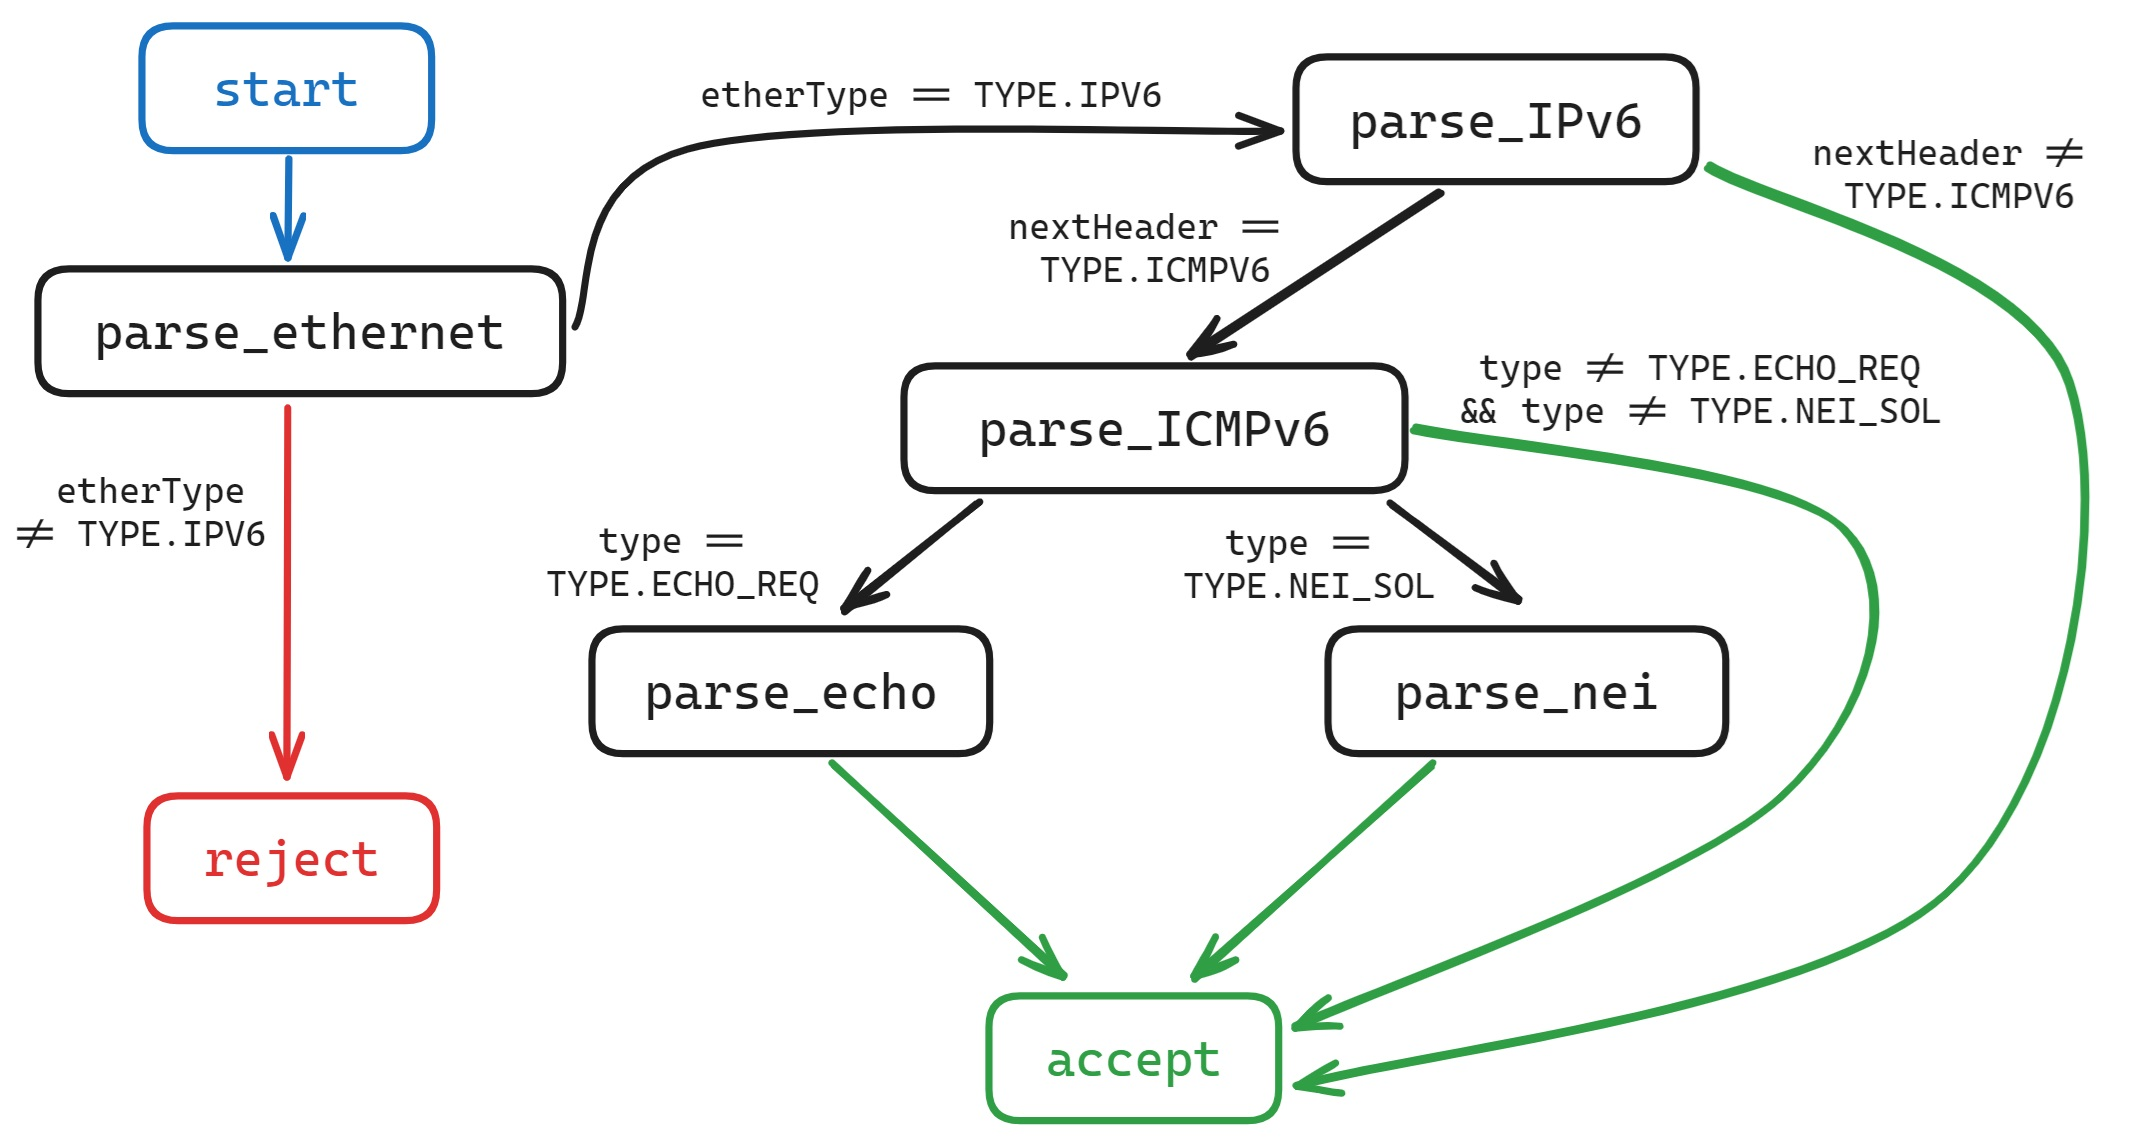
\includegraphics[width=0.85\textwidth]{figures/implementation/router6_parser.jpg}
     \caption{IPv6 router parser state machine diagram.}
     \label{fig:impl-router6parser}
\end{figure}

\textbf{Checksum Verification} ~ Depending on the packet type and destination, the ICMPv6 Checksum field may be verified. IPv6 packets that are only forwarded by the router do not have their payloads inspected. Echo Request packets directed towards the router or NS packets (regardless of their destination address, usually a node multicast address) have their checksums verified.

\textbf{Ingress processing} ~ The application block integrates the three separate control flows. First and foremost, if the Hop Limit is less than or equal to one, the Time Exceeded action is triggered. Otherwise, the program checks whether the packet is an Echo Request or an NS. If it is, the target address gets matched in the corresponding table and, in case of a match, the respective action is called. If it is an Echo Request packet whose destination address is not the router, the router checks for a match in the forwarding table. If it is an NS packet without a match in the Neighbour Responder table, it is dropped.

The router will attempt to forward any other IPv6 packet based on its destination address by performing a longest prefix match on the packet's destination address. If a match is found, the forwarding action is called, and the next hop MAC address and egress ports are defined.  If there is no match in the IPv6 forwarding table, a Destination Unreachable error message is generated. \cref{fig:impl-router6apply} illustrates the described control flow. All individual actions in the program are identical to the ones previously described.

\begin{figure}[htbp]
  \centering
    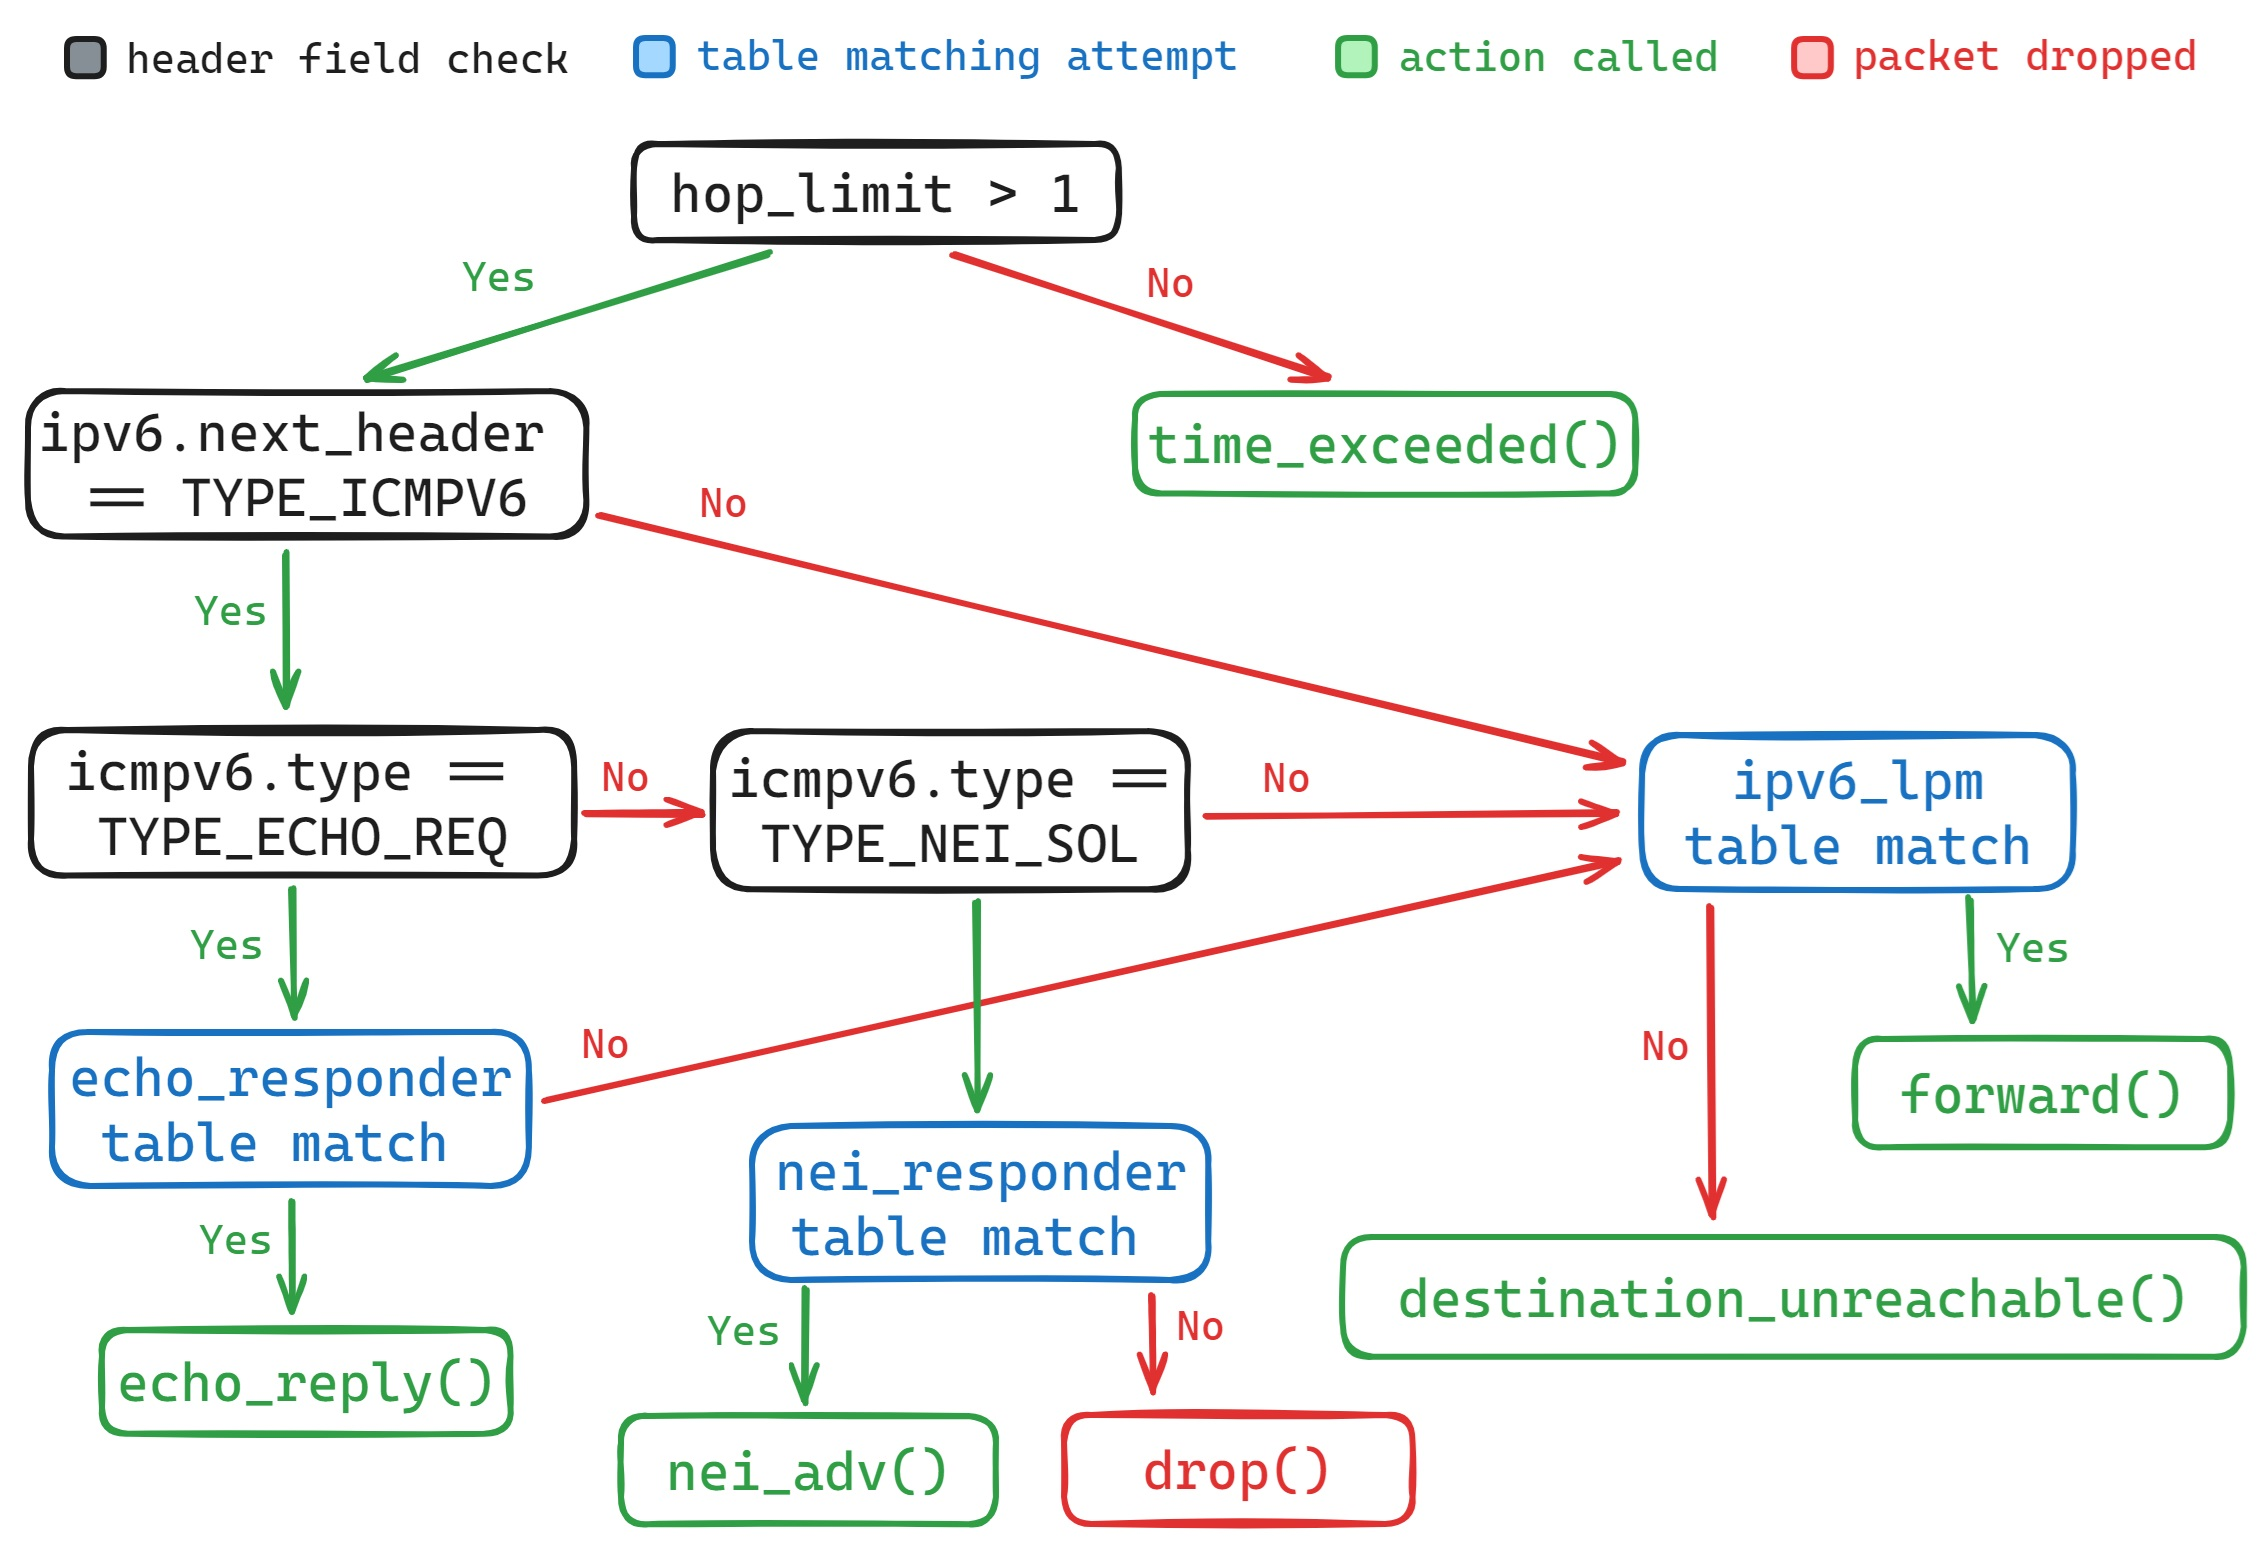
\includegraphics[width=0.9\textwidth]{figures/implementation/router6_apply.jpg}
     \caption{IPv6 router control flow represented as a simplified decision tree.}
     \label{fig:impl-router6apply}
\end{figure}

\textbf{Checksum Calculation} ~ If a response packet is generated (Echo Reply, NA, or an ICMPv6 error message), then an ICMPv6 checksum is calculated and the field updated. Otherwise, no checksum calculation is performed.

\textbf{Deparser} ~ The deparser prepends any relevant headers based on the action that has been triggered and sends the packet through the specified egress port.

This program implements IPv6 packet parsing and forwarding with the use of a longest prefix destination address matching. The router responds to Echo Requests with Echo Replies and to NSs with NAs. It also generates Time Exceeded and Destination Unreachable error messages, when appropriate. The hosts in the network can establish a connection through the router and begin to exchange packets. They can also check router availability and are made aware if a packet's Hop Limit has expired or if the router cannot find a path to the IPv6 address they are trying to reach. The program has been written such that it can easily be extended to support other ICMPv6 and NDP functionalities.


\section{Support for Both IPv4 and IPv6}
\label{sec:3.8}

As the Internet continues to grow, the adoption of IPv6 becomes more unavoidable. Currently, there exist nodes on the network which support only IPv4 or only IPv6. These nodes might still want to communicate with each other, or might need to route packets through each other to reach other nodes, and the network must be able to support these interactions. To aid in the transition from IPv4 to IPv6, mechanisms for a network to support both IPv4 and IPv6 nodes have been introduced, most notably translation, tunneling, and dual IP layering. In this section I describe all three mechanisms and explain why I chose dual IP layering for the final stage of my project.

\subsection{Translation}
\label{sec:3.8.1}

Translation of IP addresses was invented to allow hosts using the two different IPs to communicate. This mechanism depends on the existence of Address Family Border Routers (AFBRs) in the network, whose job is to translate addresses from one protocol to the other. Hosts that want to communicate with each other need to first acquire each other's aliased addresses \cite{TransitionsPaper}. For example, \cref{fig:impl-translation} depicts Host 1, using IPvX, who directs a packet towards an alias `IPvX address'. Upon reaching the AFBR, this packet gets transformed into an IPvY packet and both addresses get updated. The source address of the IPvX host is updated to its alias `IPvY address' and the destination address to its real IPvY address.

\begin{figure}[htbp]
  \centering
    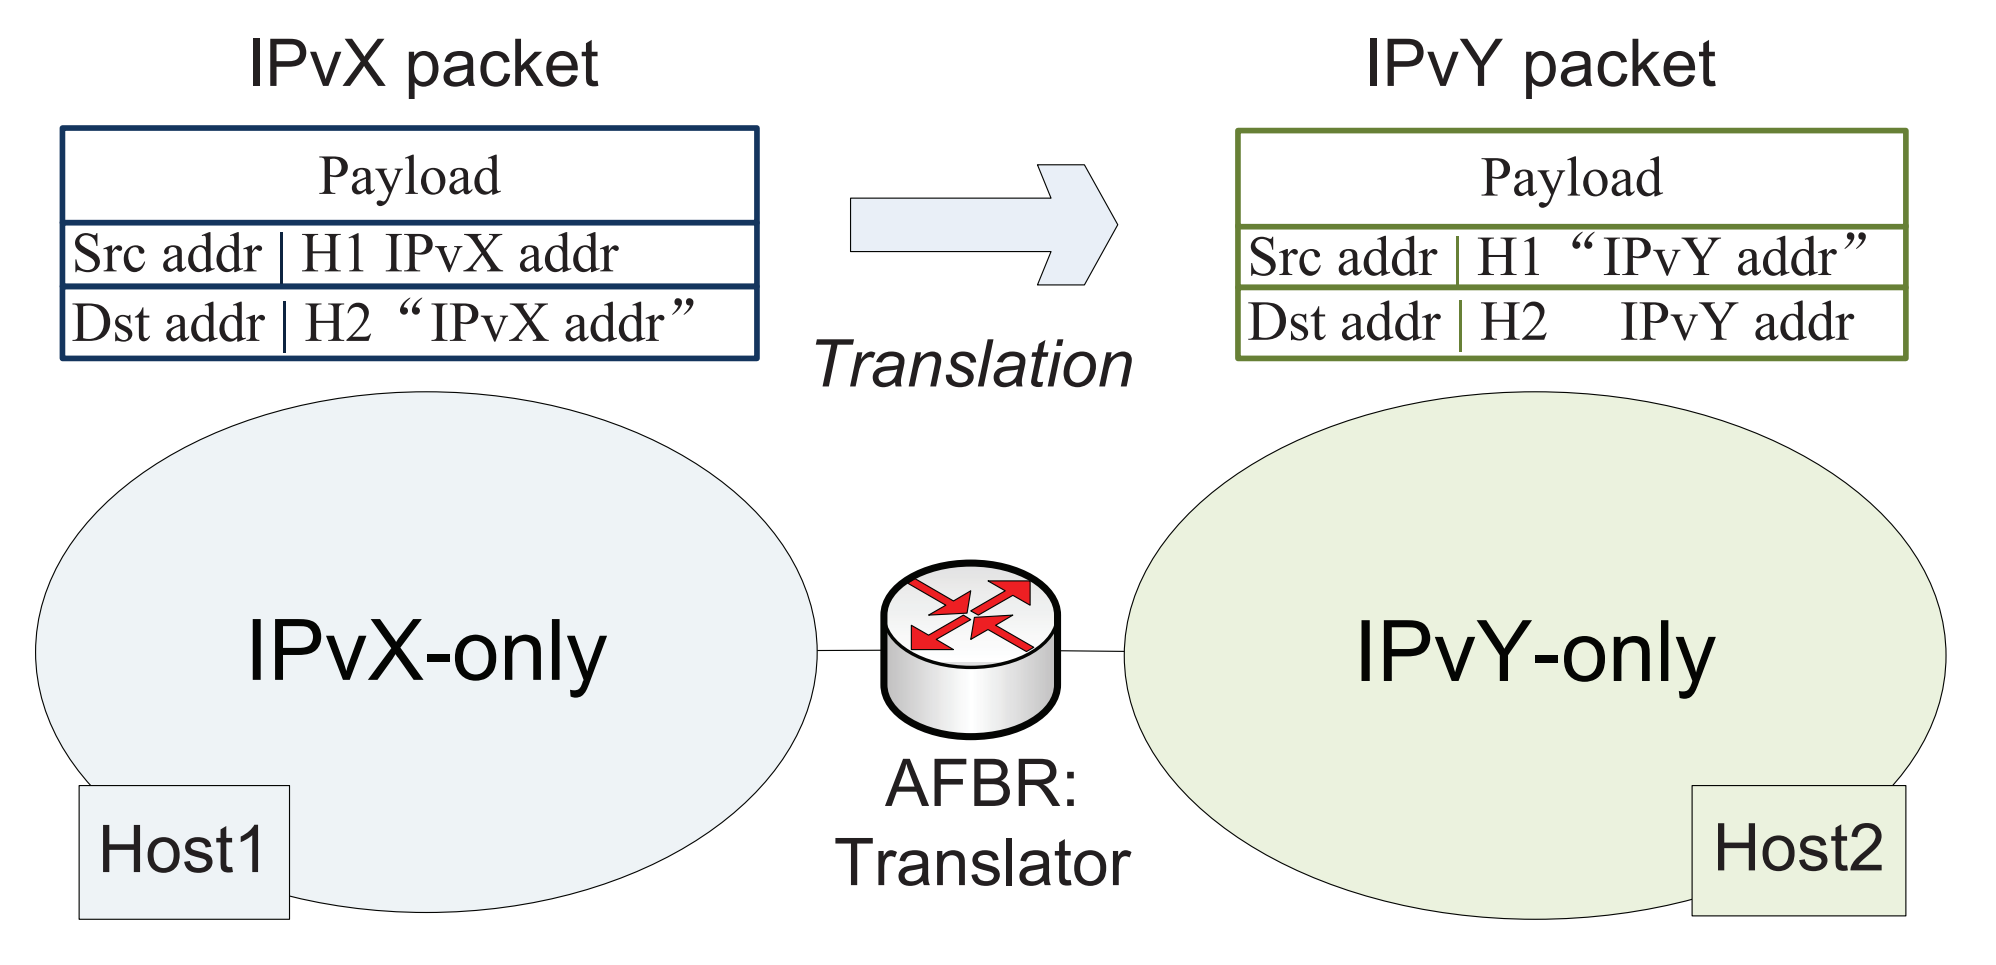
\includegraphics[width=0.5\textwidth]{figures/implementation/translation.png}
     \caption{IP translation. Taken from \cite{TransitionsPaper}.}
     \label{fig:impl-translation}
\end{figure}

The translation mechanism faces many challenges, such as guaranteeing the packet passes through an AFBR along its route; how AFBR mapping assignments are assigned; conversion of upper layer header fields (such as ICMP/TCP/UDP fields), essentially violating the end-to-end network principle; fragmentation and reassembly; and many others \cite{TransitionsPaper}. Translation does not scale well and poses many issues for networks that rely on it to support both IPs.



\subsection{Tunneling}
\label{sec:3.8.2}

Tunneling of IP packets is a mechanism used when a packet whose two end hosts use the same IP needs to pass through a portion of the network that uses a different IP \cite{Tunneling}. At the transition point between the two IP networks, an entry node encapsulates the packet by prepending a temporary IP header and leaving the original packet as a payload. The exit node removes this temporary header and forwards the packet onwards, as shown in \cref{fig:impl-tunneling} \cite{Tunneling}.

\begin{figure}[htbp]
  \centering
    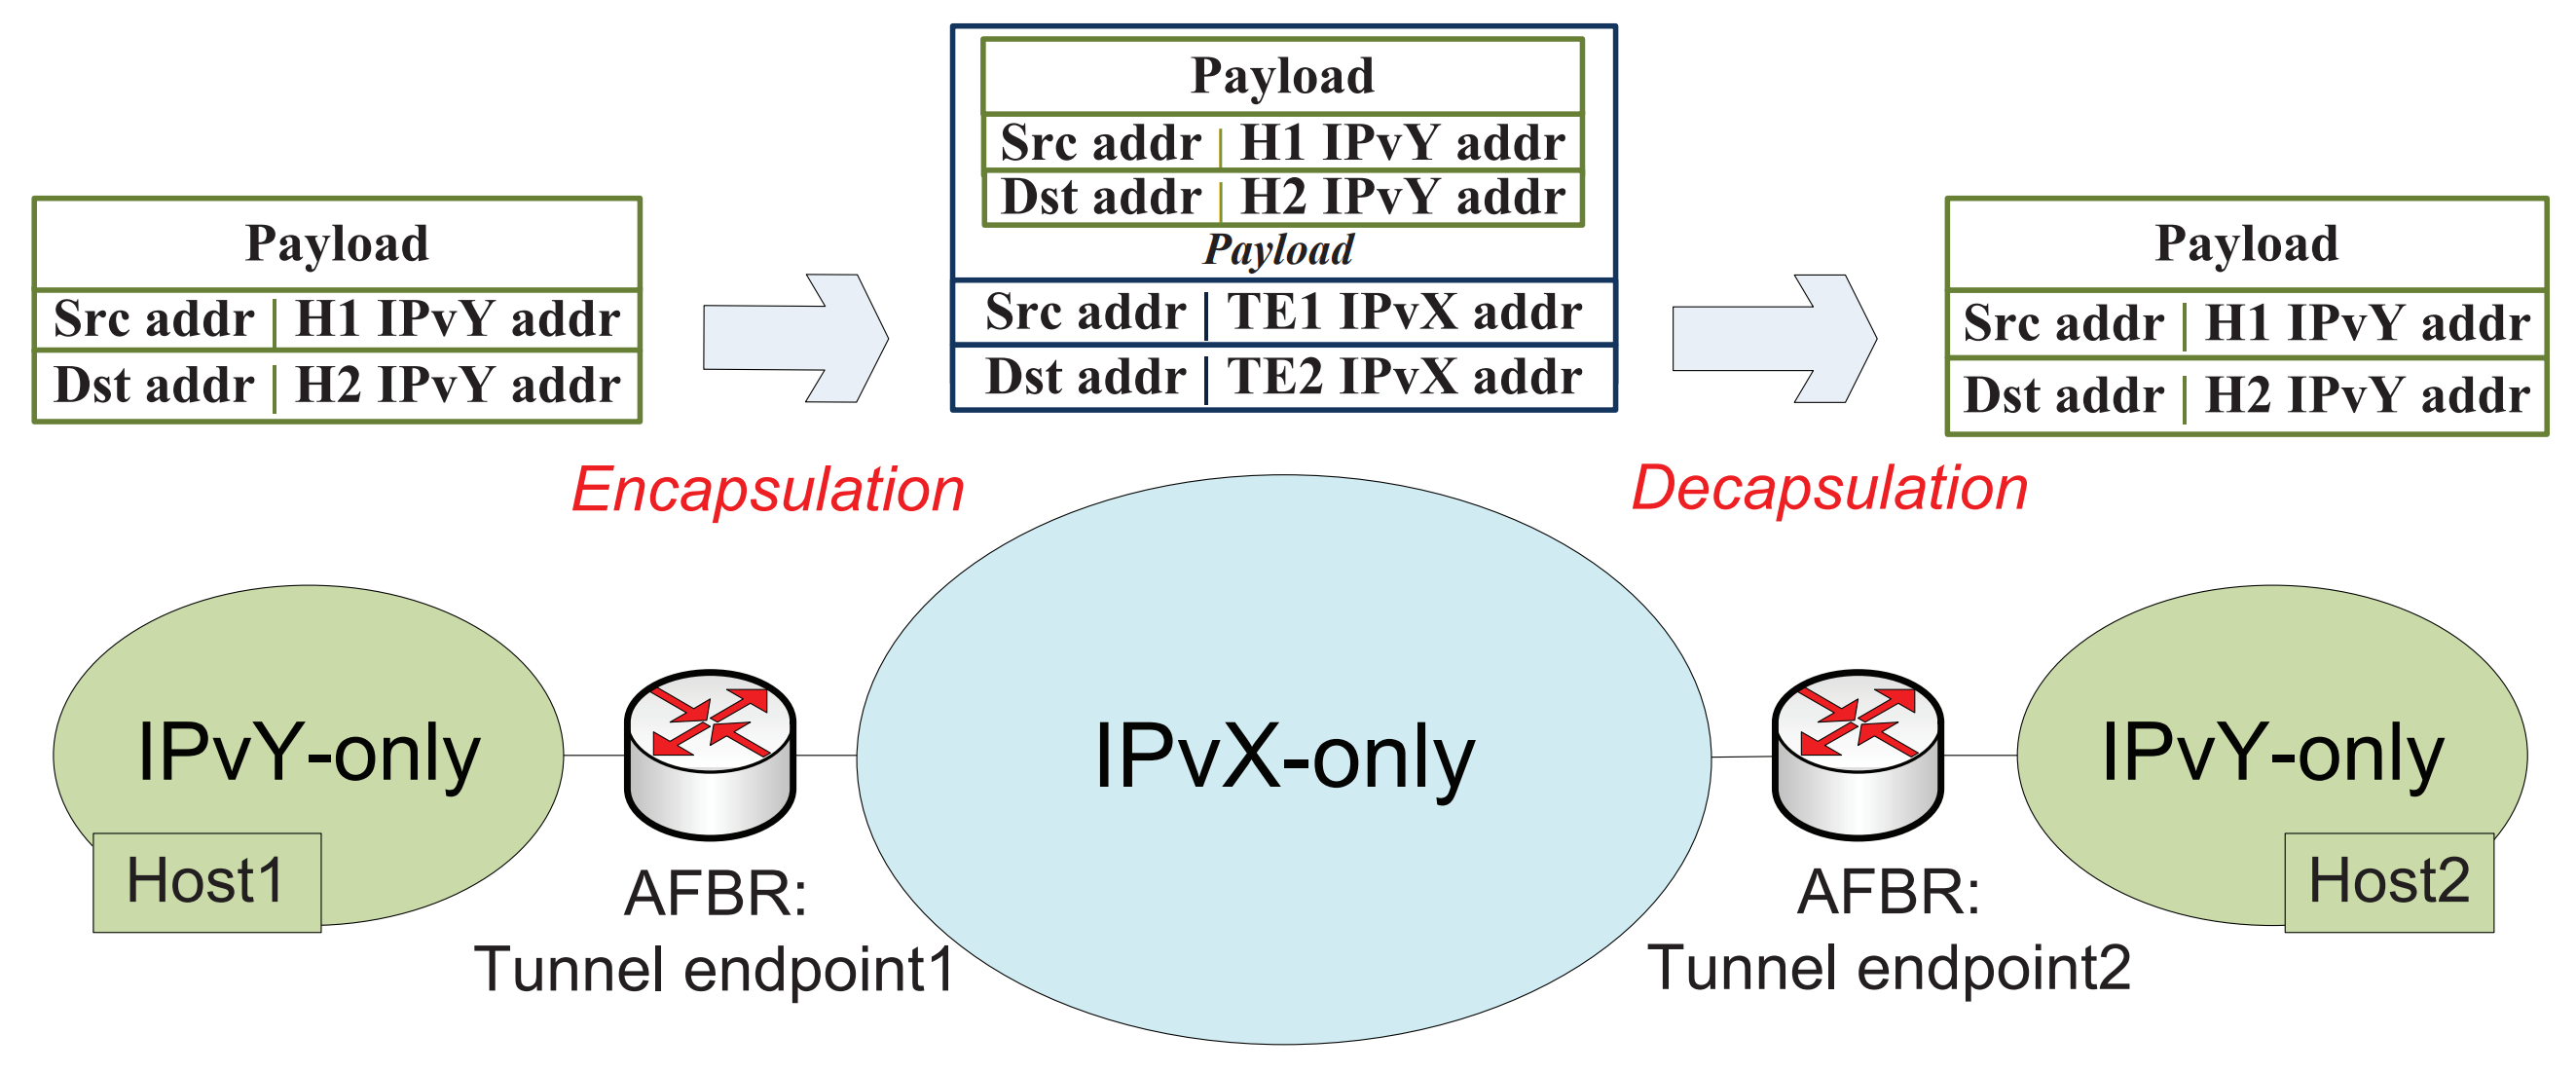
\includegraphics[width=0.6\textwidth]{figures/implementation/tunneling.png}
     \caption{IP tunneling. Taken from \cite{TransitionsPaper}.}
     \label{fig:impl-tunneling}
\end{figure}

Although tunneling is a simpler mechanism, it still faces challenges. Different types of encapsulation are required depending on the taken route, packets may need to be fragmented if they exceed the maximum size of the tunneling network, and NATs and firewalls encountered along the way may not be configured to handle encapsulated packets \cite{TransitionsPaper}.



\subsection{Dual IP Layering}
\label{sec:3.8.3}

The dual IP approach to network nodes implements two fully independent stacks, one for each IP, side-by-side. It supports separate network interfaces such that the node can identify and process both IPv4 and IPv6 \cite{DualStack}. A dual-stacked node can communicate with both IPv4 nodes and IPv6 nodes. Either stack can continue functioning even if the other is disabled \cite{DualStackSpecs}.

The dual IP approach does little to solve the IPv4 address exhaustion problem, as it still requires that a node has an IPv4 address. It does, however, ease the transition from IPv4 to IPv6 by providing separate implementations for both protocols and supporting communication with both types of nodes, and is becoming more and more widespread as IPv6 adoption is increasing \cite{DualStack}. 

For this project, I decided to provide support for both IPs by extending my IPv6 router to incorporate an IPv4 router implementation. This approach enables maximum flexibility of the node, whilst also allowing me to evaluate the functional correctness of individual IP implementations.



\section{Dual-Stack Router}
\label{sec:3.9}

My third extension is to implement support for both IPv4 and IPv6 packets. I do this by building a dual-stack router prototype. I use the IPv6 router I already built, as defined in \cref{sec:3.7}. In \cref{sec:3.9.1} I describe building a simple IPv4 router. In the remainder of this section, I explain the process of merging the two prototypes to bring to fruition a router that supports both IPv4 and IPv6.



\subsection{IPv4 Router}
\label{sec:3.9.1}

In order to obtain an IPv4 router prototype, I combine the functionalities available in the P4Pi repository into a single program, \texttt{router.p4}. There were separate P4 programs that implemented IPv4 forwarding, ARP neighbour discovery, and ICMPv4 Echo Request/Reply. Similarly to how I implemented the IPv6 router, I build a program that defines all necessary header types, combines the parser state machines and merges the ingress processing control flows. The Destination Unreachable and Time Exceeded functionalities are additional features that my IPv6 router prototype supports, but that were not included in the original IPv4 functionalities.



\subsection{Dual-Stack Router Design}
\label{sec:3.9.2}

Each host now has two IP addresses (an IPv4 and an IPv6 address) and two MAC address tables (one for ARP and one for NDP). Correspondingly, the router now has four statically defined addresses: two for each subnet. All tables in the P4 program are populated dynamically using the CLI. For more information on how to run this experiment, consult Appendix G. The program can parse and forward both IPv4 and IPv6 packets, respond to Echo Requests in both IPs, and match IP addresses to next-hop MAC addresses using ARP or NDP. On the IPv6 stack, ICMPv6 also supports two error messages.



\subsection{Dual-Stack Router Program}
\label{sec:3.9.3}

The data plane behaviour of the router is defined by the P4 file \texttt{dualstack.p4}.

\textbf{Header Definitions} ~ The \texttt{dualstack.p4} program defines a total of seven headers: Ethernet, ARP, IPv4, IPv6, ICMP, Echo, and Nei. 

\textbf{Parser} ~ The parser state machine only accepts packets that start with an Ethernet frame. It then checks the next header. ARP packets are accepted if they are an ARP Request. IPv4 and IPv6 packets are accepted regardless of what they contain, but checks are still performed in case they are ICMP packets to make sure all relevant headers are extracted. The parser’s state machine can be seen in \cref{fig:impl-dualparser}.

\begin{figure}[htbp]
  \centering
    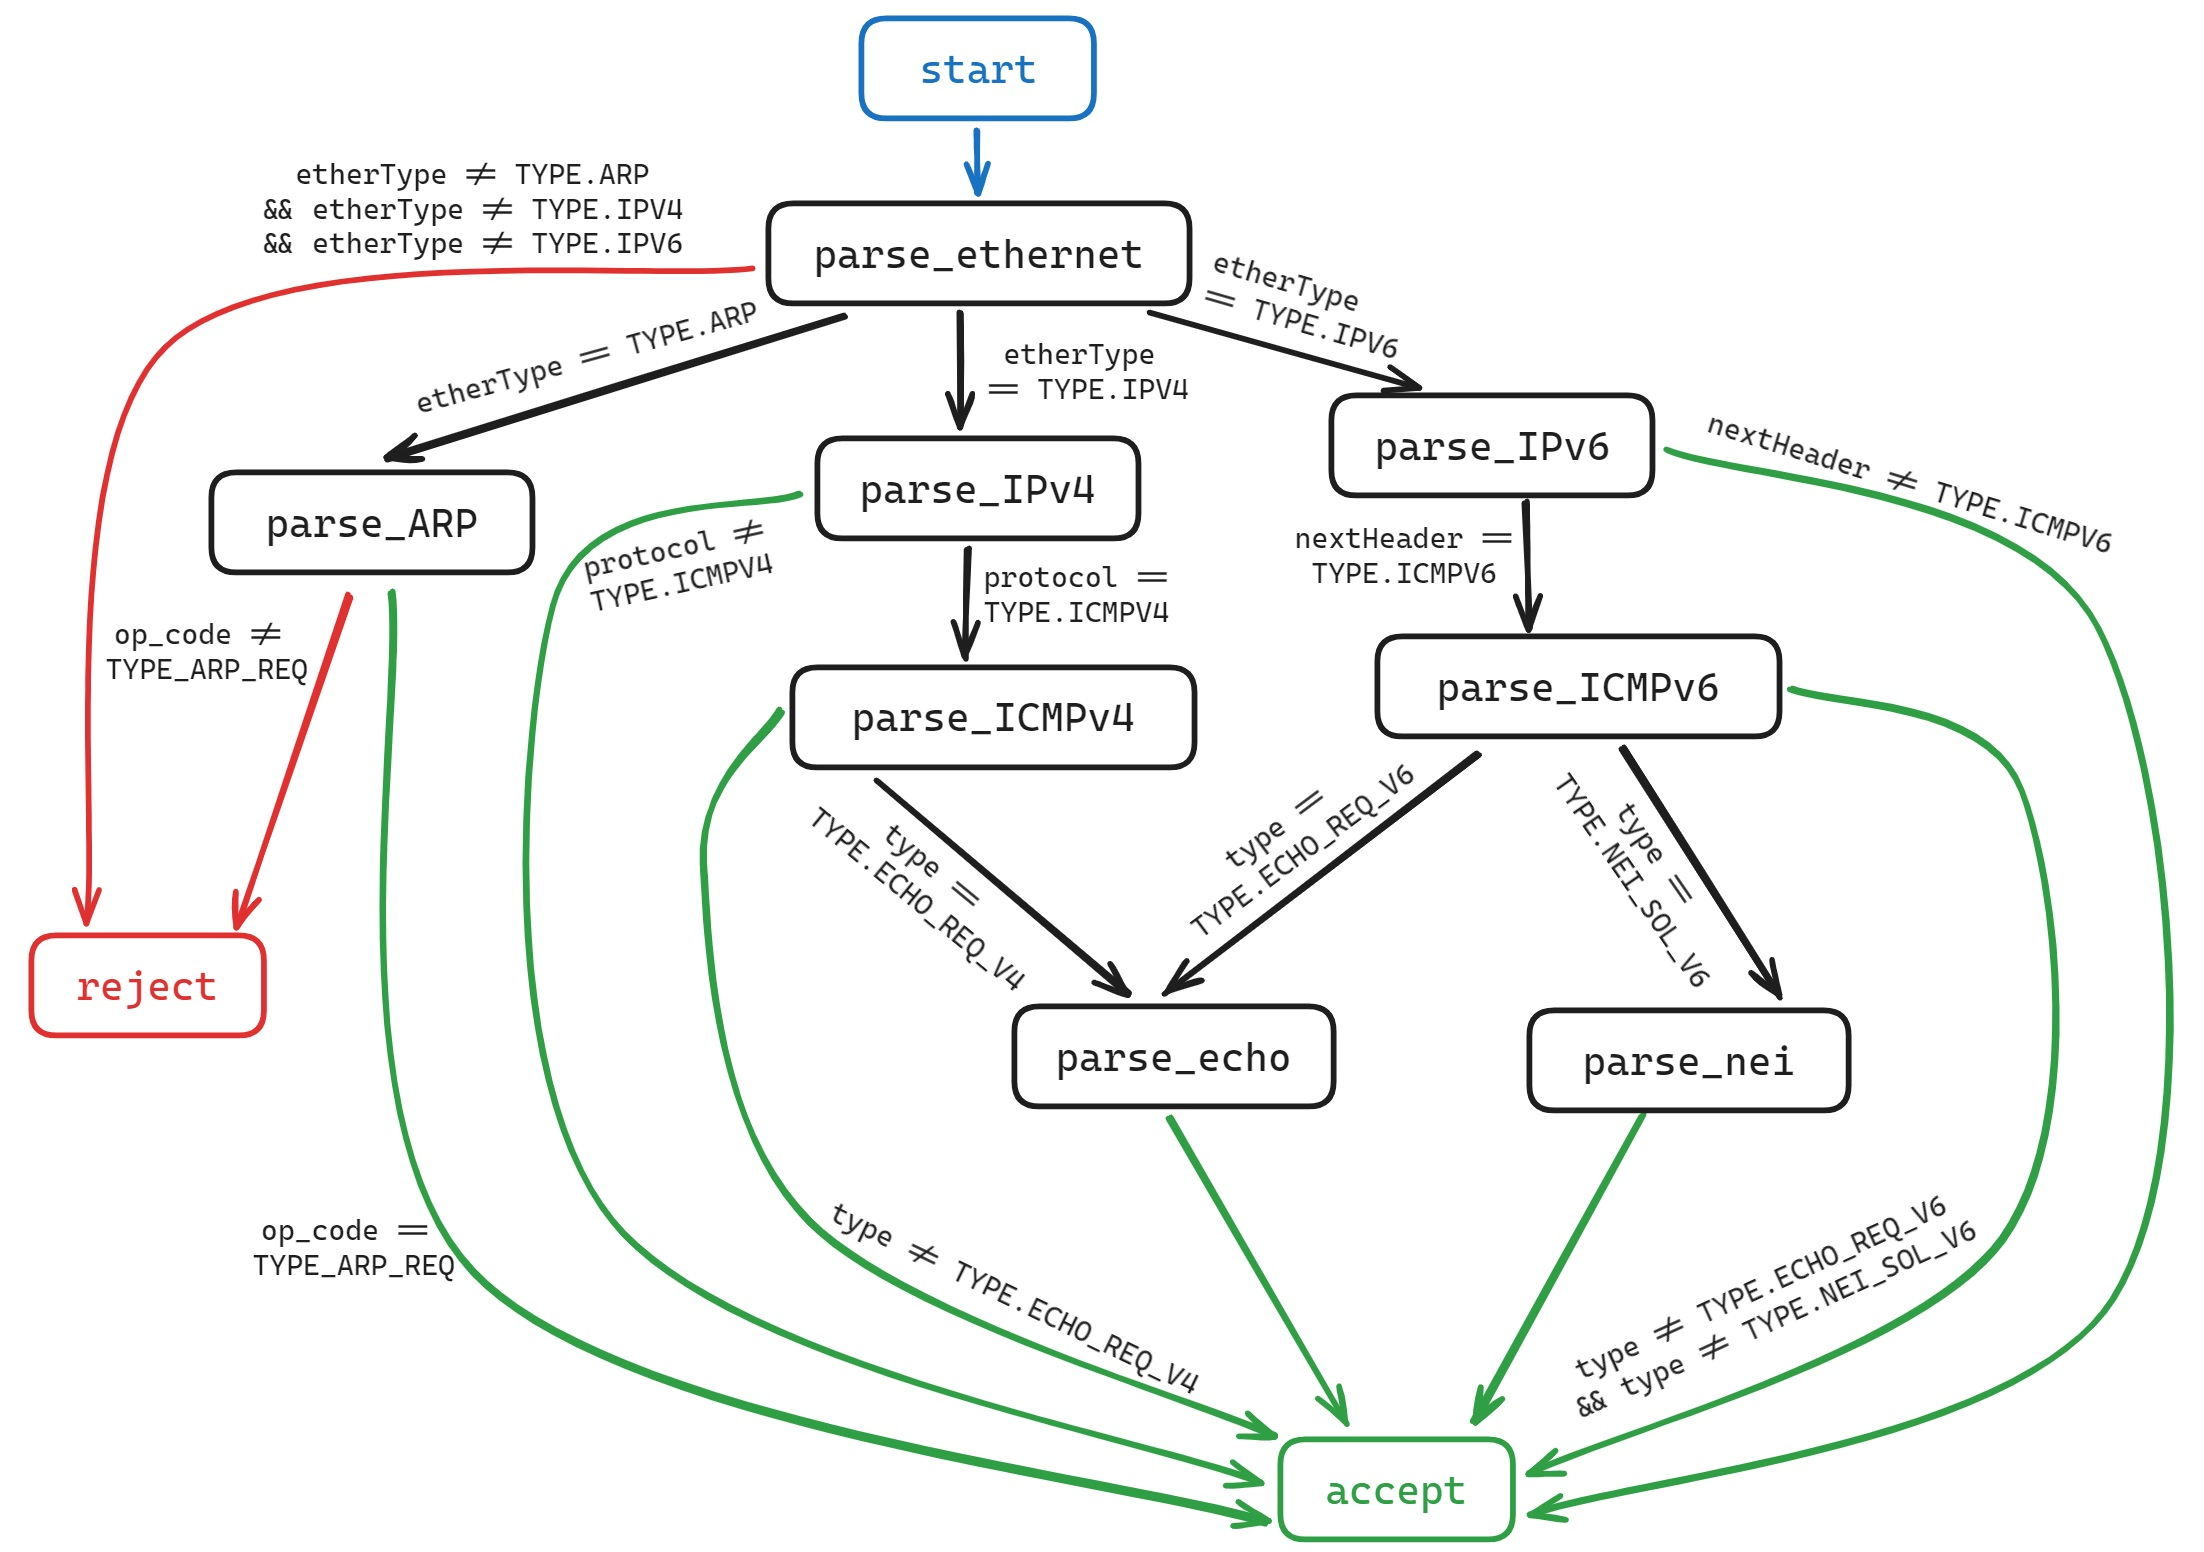
\includegraphics[width=1\textwidth]{figures/implementation/dualstack_parser.jpg}
     \caption{Dual-stack router parser state machine diagram. A packet is accepted \\ if it is of type IPv4, IPv6, or an ARP Request.}
     \label{fig:impl-dualparser}
\end{figure}

\textbf{Checksum Verification} ~ IPv4, ICMPv4 and ICMPv6 checksums are calculated and verified. Packets that are of type IPv6 and only get forwarded to their next-hop destination do not have any checksums verified.

\textbf{Ingress Processing} ~ The ingress processing of the dual-stack router represents the merging of the two control flows of the IPv4 router and the IPv6 router. If it is an ARP Request, the program looks for a match in the ARP table. If there is a hit, an ARP Reply packet is generated, containing the MAC address of the requested IPv4 address. If there is no match in the table, the packet gets dropped. If the packet has an IPv4 header, its Time To Live field gets checked first: if it is zero or one, the packet gets dropped because the IPv4 router does not have Time Exceeded error message functionality; if it is larger than one, the router checks whether the packet is an Echo Request directed towards the router. If it is, an Echo Reply is generated. Otherwise, the packet gets forwarded using an IPv4 longest prefix match table. If the packet is of type IPv6, it enters the control flow that was described in the \cref{sec:3.7}. In the end, every packet is either forwarded, dropped, an informational response is generated, or an error message is triggered. 

\begin{figure}[htbp]
  \centering
    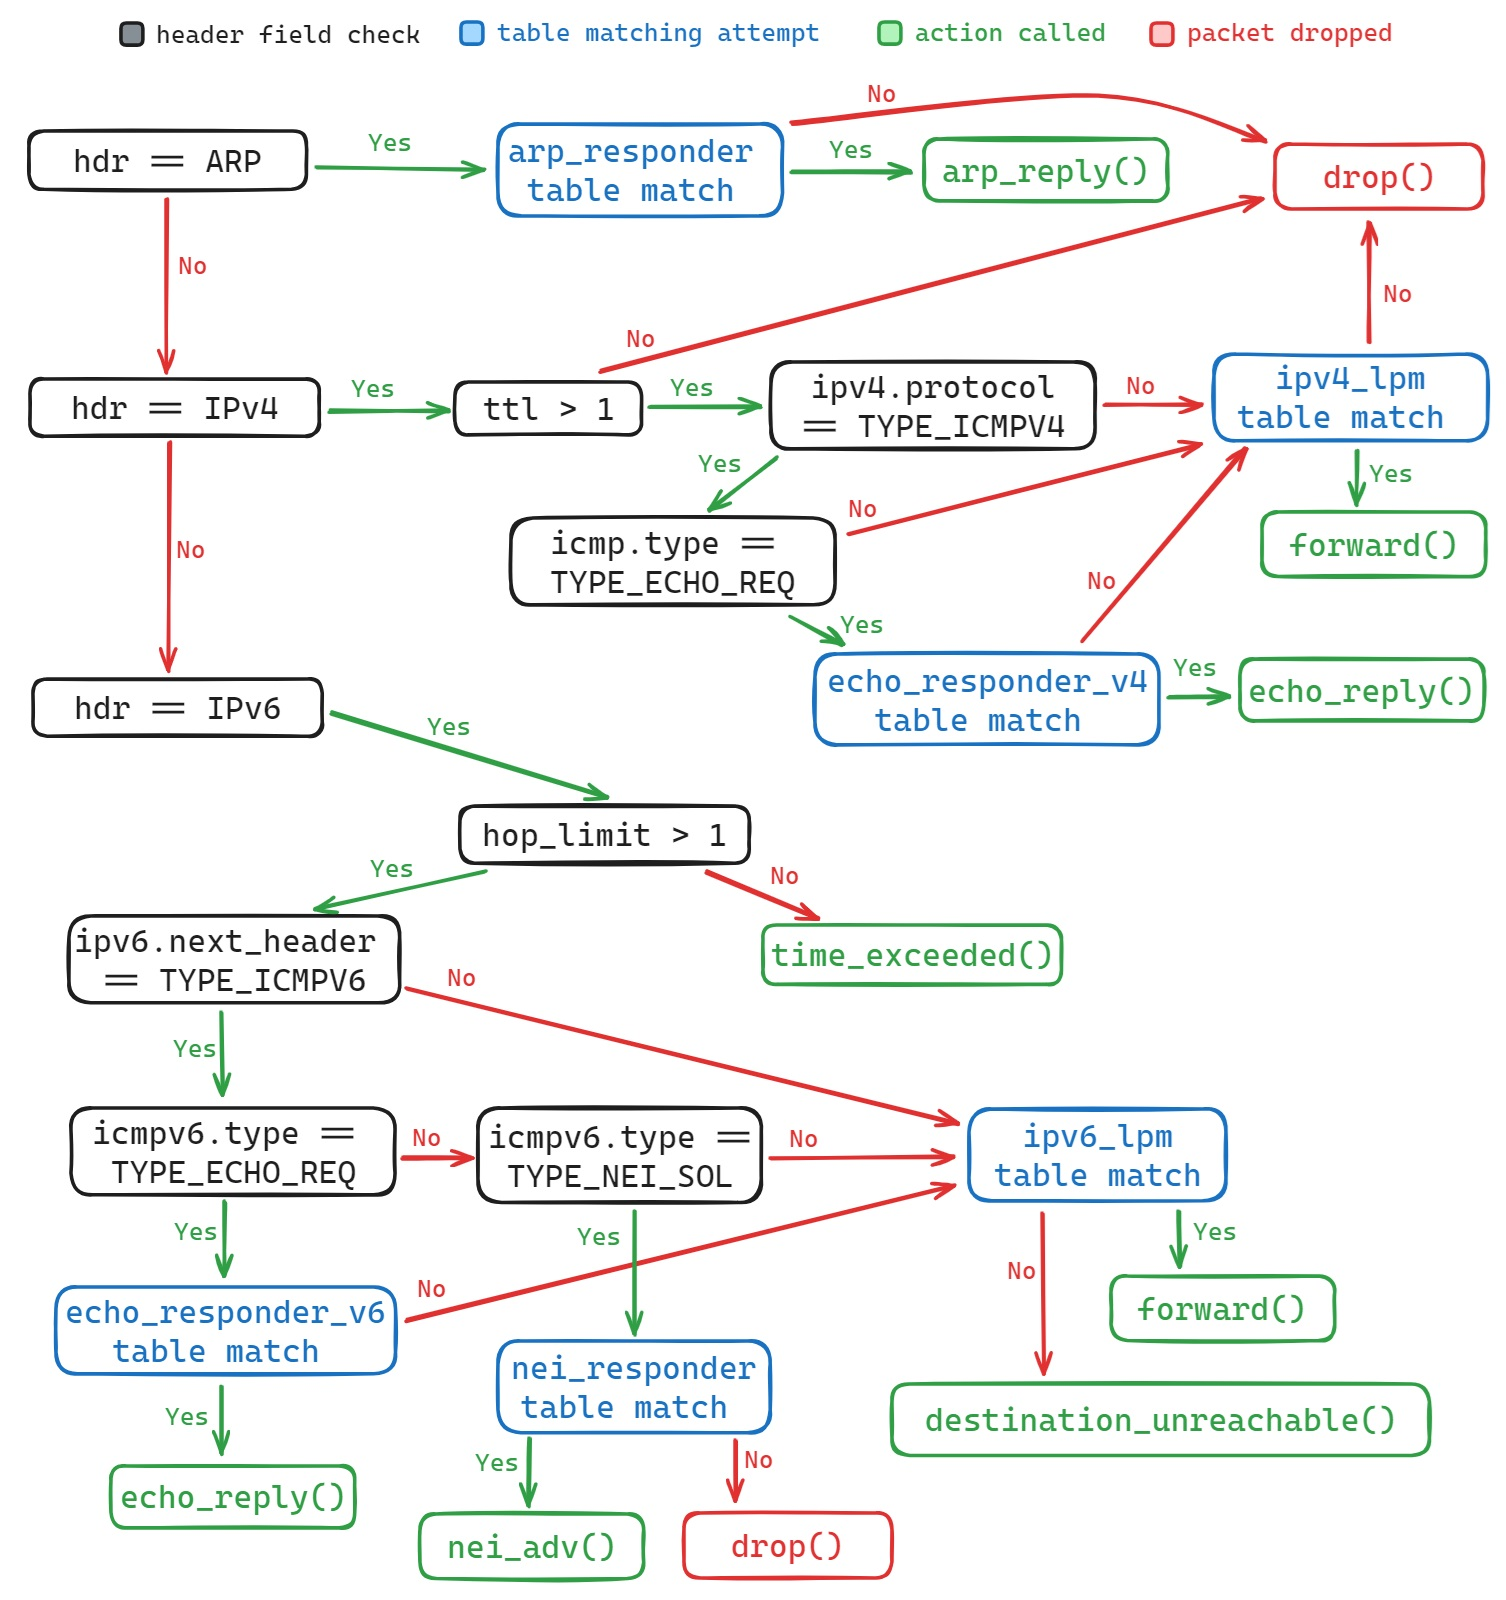
\includegraphics[width=1\textwidth]{figures/implementation/dualstack_apply.jpg}
     \caption{Dual-stack router control flow represented as a simplified decision tree.}
     \label{fig:impl-dualapply}
\end{figure}

\cref{fig:impl-dualapply} illustrates the dual-stack router's more complex control flow. Some of the action blocks have been duplicated to avoid overcomplicating the diagram. Any two blocks that share the same name refer to the same functionality. Notice the lack of a red arrow leaving the `\texttt{hdr == IPv6}' block. This is because if the packet does not match either an ARP, an IPv4 or an IPv6 header, it never would have passed the parser stage, so it must follow the green arrow out of that block.

\textbf{Checksum Calculation} ~ Any necessary IPv4, ICMPv4 or ICMPv6 checksums are recalculated and their corresponding field is updated.

\textbf{Deparser} ~ Depending on the action that was selected, the relevant headers are prepended, and the reconstructed packet is sent out the specified egress port.

This program implements both IPv4 and IPv6 forwarding, along with both ICMPv4 and ICMPv6 Echo Request/Reply. It also supports IPv4 ARP and ICMPv6 NDP. Two additional error messages are supported by ICMPv6. Hosts in the network can discover next-hop MAC addresses and exchange packets in both IPs.


\section{Implementation Summary}
\label{sec:3.10}

In this chapter I described the implementation process of building individual IPv6 router functionalities and integrating them into a fully-functional IPv6 router prototype. Every program abides by the \textit{V1Model} architecture model and defines distinct code blocks that correspond to the architecture pipeline stages. All configurations run on the \textit{simple switch} target and use the \textit{simple switch CLI} to populate the data plane tables. The functionalities were designed to mimic the packets exchanged with a working home router. As my final extension, I add an IPv4 stack in order to create a dual-stack router prototype that supports packets in both IPs. By completing these tasks, I have achieved all of my project's core objectives, along with three of the proposed extensions.

\addtocontents{lol}{\protect\vspace*{10pt}}
\chapter{Evaluation}
%TC:envir minted 1 xall 
%TC:envir algorithmic 1 xall

% Include tables in word count
%TC:envir table 0 word
%TC:envir tabular 1 word

% Include footnotes in word count
%TC:macro \footnote [text]
%TC:macro \footnotetext [text]

%TC:group minted 0 0
%TC:macro \mintinline [ignore]
%TC:macro \colb [ignore]
%TC:macro \hyperref [ignore]


\label{sec:4}

In order to evaluate my project, I take three different approaches, each of which aims to answer one of the questions outlined in \cref{sec:1.1}. \cref{sec:4.1} examines the correctness of my two router prototypes, \cref{sec:4.2} establishes adherence to the official Internet Engineering Task Force's (IETF's) network node standards, and \cref{sec:4.3} compares the performances of the IPv4-only, my IPv6-only, and my dualstack router prototype.



\section{Correctness Evaluation}
\label{sec:4.1}

In \cref{sec:3} I outlined the expected behaviour of each router functionality. These designs were based on packet exchanges with my home router and thus this section takes a test-driven approach to showing router correctness. I use the open-source packet analyser Wireshark to observe the packet exchanges between the hosts and my router prototypes \cite{Wireshark}. I use known network traffic to analyse both my IPv6 and my dual-stack routers.



\subsection{IPv6 Router}
\label{sec:4.1.1}

Both hosts start with initially empty IPv6 neighbour tables. When Host 1 sends an Echo Request to Host 2, it first sends out an NS for Host 2's IPv6 address. The router recognizes the target address and sends back an NA containing the next-hop MAC address. Host 1 places the acquired MAC address in its neighbour table and then goes forward with sending the Echo Request. An exchange of Echo Requests/Replies then begins. \cref{fig:eval-wireshark} shows the packets captured by Wireshark on Host 1's Ethernet port. The router's neighbour entry table is prepopulated and it does not send out NSs of its own. The \texttt{ping} command runs successfully both from Host 1 to Host 2, and the other way around. This exchange shows that the router is parsing and forwarding the packets correctly.

\begin{figure}[htbp]
  \centering
    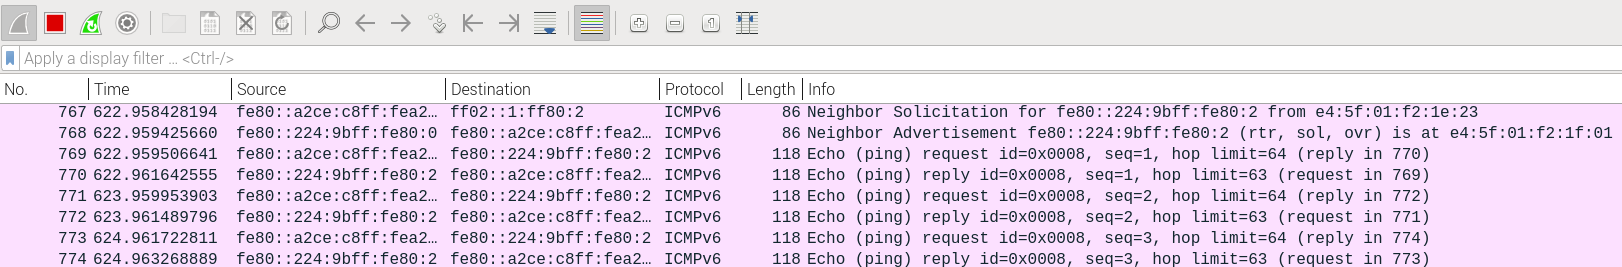
\includegraphics[width=1\textwidth]{figures/evaluation/wireshark.png}
     \caption{Packets captured by Wireshark \cite{Wireshark}. The first two packets (767-768) show \\ an NS/NA exchange with the router. The following packets (769-774) show an exchange \\ of three Echo Requests/Replies between the two hosts.}
     \label{fig:eval-wireshark}
\end{figure}

If either host sends an Echo Request to the router, a similar procedure will occur. The corresponding router subnet's MAC address will be resolved using NDP, and an exchange of Echo Requests/Replies will commence. Each Echo Request is correctly associated with its corresponding Echo Reply and no packet loss occurs. Each Echo Reply comes from the router address that is within the host’s subnet.

These two simple exchanges show that the following router functionalities are working correctly:
\begin{itemize}[topsep=0pt]
\item IPv6 packet parsing (as designed in \cref{sec:3.4.2});
\item IPv6 packet forwarding to a different host (as designed in \cref{sec:3.4.2});
\item ICMPv6 Echo Reply is generated in response to an Echo Request for a router address (as designed in \cref{sec:3.5.2});
\item NDP NA is generated in response to an NS (as designed in \cref{sec:3.6.2}).
\end{itemize}

Two more ICMPv6 functionalities need to be tested, namely the error messages: Time Exceeded and Destination Unreachable. An example test is shown in \cref{fig:eval-timeextest}, where an Echo Request is sent with a Hop Limit of 1. Regardless of what the destination of the Echo Request is, the Time Exceeded error message has the router as its source address, since that is the node at which the Hop Limit expired.
 
\begin{figure}[htbp]
  \centering
    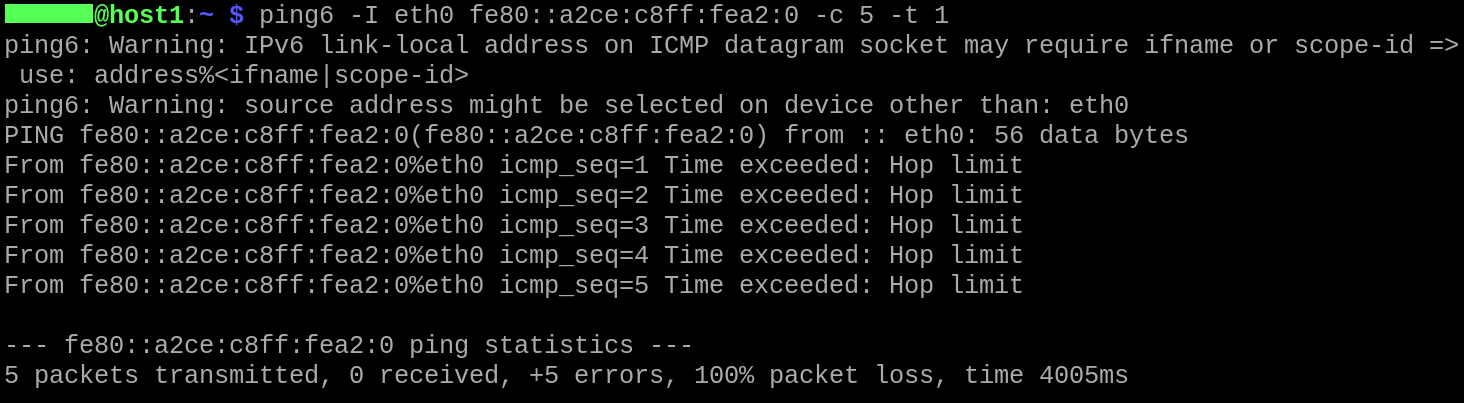
\includegraphics[width=1\textwidth]{figures/evaluation/icmpv6_test2.png}
     \caption{ICMPv6 Time Exceeded error message test.}
     \label{fig:eval-timeextest}
\end{figure}

The Destination Unreachable address requires an extra step to test. If I attempt to ping a random address, I get a Destination Unreachable Code 3 (Address Unreachable) error message from the host itself. This is because the host will send out an NS for this address, but will receive no NA from the router. To get around this, I have to manually define a neighbour table entry for the chosen IPv6 address. Running the \texttt{ping} command then directly sends the Echo Request. The router receives it, and checks its forwarding table to try and find a match for the IPv6 address. When it fails, it sends back a Destination Unreachable Code 0 (No Route to Destination) error message.

It is important to note that depending on which host is conducting these tests, it receives responses from the router address corresponding to the host's subnet. 

These two experiments show that the rest of the router functionalities are performed correctly (all of which were described in \cref{sec:3.5.2}):
\begin{itemize}[topsep=0pt]
\item ICMPv6 Time Exceeded message is generated in response to a Hop Limit expiring;
\item ICMPv6 Destination Unreachable (No Route to Destination) message is generated in response to a miss in the IPv6 forwarding table;
\item Error messages sent back to hosts are sent out the correct router subnet port.
\end{itemize}



\subsection{Dual-Stack Router}
\label{sec:4.1.2}

I run the same tests to establish the correctness of the IPv6 part of the dual-stack router. Similar tests are conducted to verify the IPv4 implementation: ARP Request/Reply, IPv4 forwarding and parsing, ICMPv4 Echo Request/Reply. The P4Pi repository has no ICMPv4 error message functionalities, so those are not tested. Only the IPv6 half of the dual-stack router implements Time Exceeded and Destination Unreachable error messages.

When using the dual-stack router, hosts in the network can send both IPv4 and IPv6 packets to each other, as well as to the router. They can find the next-hop MAC addresses of other devices in the network through either ARP or NDP, and ping both IP router addresses in their respective subnets. The test example below shows that a \texttt{ping} command from Host 1 to Host 2 is successful in eliciting a response in both IPs.

\begin{figure}[htbp]
  \centering
    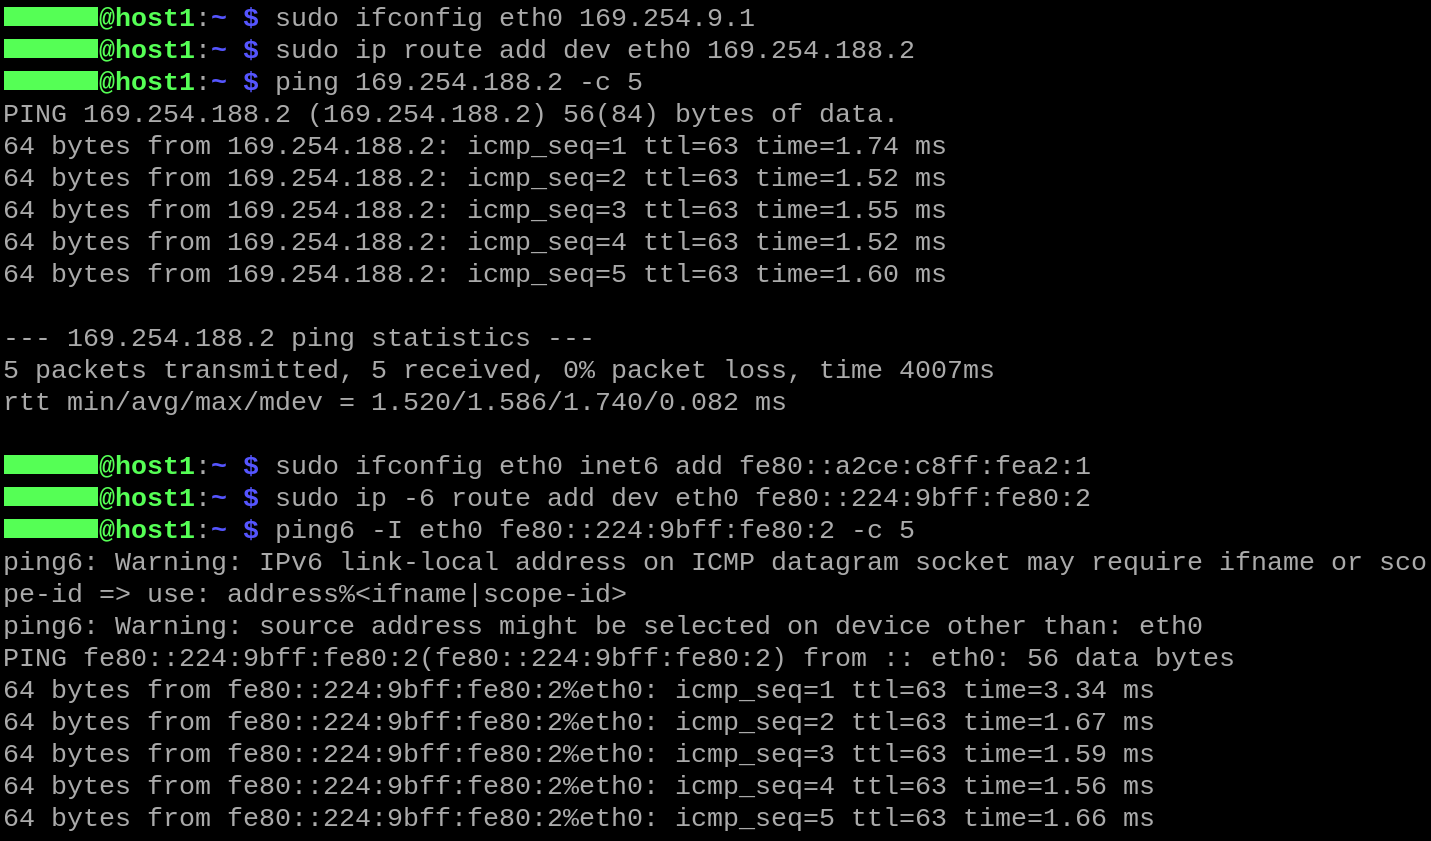
\includegraphics[width=1\textwidth]{figures/evaluation/dualstack_test.png}
     \caption{Dual-stack router successfully forwards both IPv4 and IPv6 packets.}
     \label{fig:eval-dualtest}
\end{figure}



\subsection{Correctness Summary}
\label{sec:4.1.}

This section evaluated and demonstrated the correctness of my router prototype, using the expectations I outlined when building each functionality as a baseline. I test each component and show that it adheres to my individual functionality designs. My final IPv6 router properly parses, forwards and responds to IPv6 packets. It identifies and generates both ICMPv6 and NDP messages. The dual-stack router properly differentiates between IPv4 and IPv6 packets and processes them accordingly. 

By observing the behaviour of both router prototypes through packets captured by Wireshark, I also confirm that checksums are calculated correctly, no packet duplication occurs, and hosts only receive packets which are meant to be received by them.



\section{Standards Compliance Evaluation}
\label{sec:4.2}

In order to functionally evaluate my project, I use the official specifications provided by the IETF Request for Comments (RFC) documentations on IPv6, ICMPv6, NDP, and Dual IP Layering \cite{IPv6Specs, ICMPv6Specs, NDPSpecs, DualStackSpecs}. I compare my router's behaviour with the provided baselines to establish the functional correctness of my project. In \cref{sec:4.2.1} I explain why I chose to use the IETF RFCs as guidelines. In \cref{sec:4.2.2} I provide a general overview of the handling of IPv6 and ICMPv6 packets, as well as the implemented dual-stack functionalities, followed by an in-depth look at specific ICMPv6 message specifications and whether they have been fulfilled in \cref{sec:4.2.3}.



\subsection{What are the IETF RFCs?}
\label{sec:4.2.1}

The Internet Engineering Task Force (IETF) is `the premier standards development organization (SDO) for the Internet', and the Requests For Comments (RFCs) are the IETF's technical documentations \cite{IETFIntro}. The standards produced by the IETF are not obligatory, but are considered best practice by the networking community, and are often adopted by Internet users \cite{IETFIntro}.



\subsection{General Functionalities}
\label{sec:4.2.2}

The following three tables explore the basic router characteristics that I have extracted from the respective specifications. Most of them are intuitive, such as adhering to the defined packet formats or discarding packets that do not fulfil necessary requirements.

\begin{table}[htbp]
    \centering
    \renewcommand{\arraystretch}{1.25}
    \begin{tabular}{|p{125mm}|l|}
    \hline
    \textbf{IETF Specification} & \textbf{Fulfilled?} \\
    \hline
    Supports a link-layer communication facility (Ethernet). & \makecell{\textcolor[RGB]{0,150,0}{\textbf{yes}}} \\
    \hline
    Is consistent with the defined IPv6 header format. & \makecell{\textcolor[RGB]{0,150,0}{\textbf{yes}}} \\
    \hline
    Discards packets that have malformed IPv6 headers. & \makecell{\textcolor[RGB]{0,150,0}{\textbf{yes}}} \\
    \hline
    Supports IPv6 extension header formats. & \makecell{\textcolor[RGB]{200,0,0}{\textbf{no}}} \\
    \hline
    Does not perform checksum verifications or calculations. & \makecell{\textcolor[RGB]{0,150,0}{\textbf{yes}}} \\
    \hline
    Parses, responds to, and forwards packets based on their type, destination address, and data plane forwarding table. & \makecell{\textcolor[RGB]{0,150,0}{\textbf{yes}}} \\
    \hline
    Discards a packet if the Hop Limit is 0 or gets decremented to 0. & \makecell{\textcolor[RGB]{0,150,0}{\textbf{yes}}} \\
    \hline
    Does not support fragmentation. & \makecell{\textcolor[RGB]{0,150,0}{\textbf{yes}}} \\
    \hline
    \end{tabular}
    \caption{IPv6 general specifications \cite{IPv6Specs}.}
    \label{table:eval-ipv6gen}
\end{table}

\begin{table}[htbp]
    \centering
    \renewcommand{\arraystretch}{1.25}
    \begin{tabular}{|p{125mm}|l|}
    \hline
    \textbf{IETF Specification} & \textbf{Fulfilled?} \\
    \hline
    Is consistent with the defined ICMPv6 header format. & \makecell{\textcolor[RGB]{0,150,0}{\textbf{yes}}} \\
    \hline
    Discards packets that have malformed ICMPv6 headers. & \makecell{\textcolor[RGB]{0,150,0}{\textbf{yes}}} \\
    \hline
    Verifies and calculates checksums using an IPv6 pseudoheader. & \makecell{\textcolor[RGB]{0,150,0}{\textbf{yes}}} \\
    \hline
    Uses type codes 0-127 for informational messages. & \makecell{\textcolor[RGB]{0,150,0}{\textbf{yes}}} \\
    \hline
    Uses type codes 128-255 for error messages. & \makecell{\textcolor[RGB]{0,150,0}{\textbf{yes}}} \\
    \hline
    Supports a multitude of ICMPv6 message packets. & \makecell{\textcolor[RGB]{0,150,0}{\textbf{yes}}} \\
    \hline
    \end{tabular}
    \caption{ICMPv6 general specifications \cite{ICMPv6Specs}.}
    \label{table:eval-icmpmv6gen}
\end{table}

\begin{table}[htbp]
    \centering
    \renewcommand{\arraystretch}{1.25}
    \begin{tabular}{|p{125mm}|l|}
    \hline
    \textbf{IETF Specification} & \textbf{Fulfilled?} \\
    \hline
    Has the ability to send and receive both IPv4 and IPv6 packets. & \makecell{\textcolor[RGB]{0,150,0}{\textbf{yes}}} \\
    \hline
    Provides independent correct implementations of an IPv4 node and an IPv6 node. & \makecell{\textcolor[RGB]{0,150,0}{\textbf{yes}}} \\
    \hline
    Provides a configuration switch to disable either the IPv4 or IPv6
    stack (optional). & \makecell{\textcolor[RGB]{200,0,0}{\textbf{no}}} \\
    \hline
    \end{tabular}
    \caption{Dual-stack general specifications \cite{DualStackSpecs}}
    \label{table:eval-dualstackgen}
\end{table}

All basic IPv6 functionalities have been fulfilled, with the exception of extension header formats, as seen in \cref{table:eval-ipv6gen}. The last requirement in the ICMPv6 specifications, \cref{table:eval-icmpmv6gen}, has been marked as `yes' because multiple different ICMPv6 messages have been implemented and the framework for implementing additional messages has been established. This is discussed further in the next section. The dual-stack specifications requirements can be seen in \cref{table:eval-dualstackgen}



\subsection{Specific Message Functionalities}
\label{sec:4.2.3}

The official ICMPv6 specifications define six types of ICMPv6 message: two informational messages (Echo Request and Echo Reply), and four error messages (Destination Unreachable, Packet Too Big, Time Exceeded, and Parameter Problem). As previously described, my IPv6 router implements four of these message types and discards all other ICMPv6 packet types. A breakdown of the required functionalities for these four messages can be seen in the respective tables (\cref{table:eval-destunr}, \cref{table:eval-timeexc}, \cref{table:eval-echo}). All requirements are fulfilled with the exception of an Echo Response to a multicast destination address. My router only responds to unicast Echo Requests. 

The official IPv6 NDP specifications define the expected NDP functionalities of a router. My router responds to NSs with NAs, but its own neighbour entry tables are prepopulated by the control plane, rather than by using NSs. The breakdown of the IETF's requirements for this message pair can be seen in \cref{table:eval-ndpnei}.

In all tables, I use the keywords `MUST' and `SHOULD', as defined by the IETF \cite{KeyWordsSpecs}.

\begin{table}[htbp]
    \centering
    \renewcommand{\arraystretch}{1.25}
    \begin{tabular}{|p{125mm}|l|}
    \hline
    \textbf{IETF Specification} & \textbf{Fulfilled?} \\
    \hline
    A Destination Unreachable message SHOULD be generated by a router in response to a packet that cannot be delivered to its destination address for reasons other than congestion. & \makecell{\textcolor[RGB]{0,150,0}{\textbf{yes}}} \\
    \hline
    If the reason for the failure to deliver is lack of a matching entry in the forwarding node's routing table, the Code field MUST be set to 0. & \makecell{\textcolor[RGB]{0,150,0}{\textbf{yes}}} \\
    \hline
    \end{tabular}
    \caption{ICMPv6 Destination Unreachable specifications \cite{ICMPv6Specs}.}
    \label{table:eval-destunr}
\end{table}

\begin{table}[htbp]
    \centering
    \renewcommand{\arraystretch}{1.25}
    \begin{tabular}{|p{125mm}|l|}
    \hline
    \textbf{IETF Specification} & \textbf{Fulfilled?} \\
    \hline
    If a router receives a packet with a Hop Limit of zero, or if a
    router decrements a packet's Hop Limit to zero, it MUST discard the packet. & \makecell{\textcolor[RGB]{0,150,0}{\textbf{yes}}} \\
    \hline
    The router must also originate an ICMPv6 Time Exceeded message with Code 0 to the source of the packet. & \makecell{\textcolor[RGB]{0,150,0}{\textbf{yes}}} \\
    \hline
    \end{tabular}
    \caption{ICMPv6 Time Exceeded specifications \cite{ICMPv6Specs}.}
    \label{table:eval-timeexc}
\end{table}

\begin{table}[htbp]
    \centering
    \renewcommand{\arraystretch}{1.25}
    \begin{tabular}{|p{125mm}|l|}
    \hline
    \textbf{IETF Specification} & \textbf{Fulfilled?} \\
    \hline
    Every node MUST implement an ICMPv6 Echo responder function that receives Echo Requests and originates corresponding Echo Replies. & \makecell{\textcolor[RGB]{0,150,0}{\textbf{yes}}} \\
    \hline
    The source address of an Echo Reply sent in response to a unicast Echo Request message MUST be the same as the destination address of that Echo Request message. & \makecell{\textcolor[RGB]{0,150,0}{\textbf{yes}}} \\
    \hline
    An Echo Reply SHOULD be sent in response to an Echo Request message sent to an IPv6 multicast or anycast address.  In this case, the source address of the reply MUST be a unicast address belonging to the interface on which the Echo Request message was received.  & \makecell{\textcolor[RGB]{200,0,0}{\textbf{no}}} \\
    \hline
    The data received in the ICMPv6 Echo Request message MUST be returned entirely and unmodified in the ICMPv6 Echo Reply message. & \makecell{\textcolor[RGB]{0,150,0}{\textbf{yes}}} \\
    \hline
    \end{tabular}
    \caption{ICMPv6 Echo Request/Reply specifications \cite{ICMPv6Specs}.}
    \label{table:eval-echo}
\end{table}

\begin{table}[h!tbp]
    \centering
    \renewcommand{\arraystretch}{1.25}
    \begin{tabular}{|p{125mm}|l|}
    \hline
    \textbf{IETF Specification} & \textbf{Fulfilled?} \\
    \hline
    Nodes MUST send Neighbour Advertisements in response to Neighbour Solicitations if they have the target link-layer address in their cache. & \makecell{\textcolor[RGB]{0,150,0}{\textbf{yes}}} \\
    \hline
    The link-layer address for the target option, i.e., the sender of the advertisement, MUST be included on link layers that have addresses when responding to multicast solicitations. & \makecell{\textcolor[RGB]{0,150,0}{\textbf{yes}}} \\
    \hline
    The link-layer address for the target option SHOULD be included when responding to a unicast Neighbour Solicitation. & \makecell{\textcolor[RGB]{0,150,0}{\textbf{yes}}} \\
    \hline 
    A router MUST send out Neighbour Solicitations to acquire link-layer addresses. & \makecell{\textcolor[RGB]{200,0,0}{\textbf{no}}} \\
    \hline 
    \end{tabular}
    \caption{NDP Neighbour Solicitation/Advertisement specifications \cite{NDPSpecs}.}
    \label{table:eval-ndpnei}
\end{table}



\subsection{Standards Compliance Summary}
\label{sec:4.2.4}

This section evaluated whether my routers adhere to the Internet's established best practices, as outlined by the IETF. My router prototypes fulfil all mandatory characteristics of the developed functionalities. Furthermore, my prototypes can easily be extended to implement any additional components, as the core requirements for each protocol have already been built.



\section{Performance Evaluation}
\label{sec:4.3}

In order to compare the performances of the IPv4, IPv6 and dual-stack router prototypes, I simulate network traffic with Echo Request/Reply pairs. I initially sent 100 Echo Request packets from Host 1 to both the router and Host 2, but noticed that the first RTT was always an outlier and, with the help of Wireshark, realised that this is because the hosts' MAC address caches are initially empty. I also noticed unusually high standard deviations, likely caused by the cold cache RTTs. For these reasons, I decided to run two separate experiments: a warm cache experiment and a cold cache experiment. My experiments have limitations, such as each subnet being made up of only one host and the close proximity of the three network nodes. The most important limitation, however, is that I cannot identify the exact points in the network that cause the latency I measure. Different components of every network affect latency differently, often unexpectedly, even when running under identical conditions \cite{LatencyPaper}.



\subsection{Warm Cache Echo Request/Reply}
\label{sec:4.3.1}

The mean warm cache RTTs from 250 Echo Request/Reply pairs are summarized in \cref{table:eval-ping}. The gathered statistics show that the RTTs in both the host-to-host and the host-to-router scenarios are comparable. All four configurations average within the same 150 $\mu$s timespan. \cref{fig:eval-pingWC} shows the cumulative distribution of the warm cache RTTs in a host-to-host exchange and a host-to-router exchange, respectively.

\begin{table}[htbp]
    \centering
    \renewcommand{\arraystretch}{1.25}
    \begin{tabular}{|c|c|c|c|c|}
    \hline
    \multirow{2}{*}{\textbf{IP Protocol}} & \multicolumn{2}{c|}{\textbf{Host-to-Host}} & \multicolumn{2}{c|}{\textbf{Host-to-Router}}\\
    \cline{2-5}
     & \textbf{Single-stack} & \textbf{Dual-stack} & \textbf{Single-stack} & \textbf{Dual-stack}\\
    \hline
    IPv4 & 1.473 $\pm$ 0.128 & 1.531 $\pm$ 0.122 & 0.971 $\pm$ 0.128 & 0.994 $\pm$ 0.108 \\
    IPv6 & 1.544 $\pm$ 0.128 & 1.602 $\pm$ 0.150 & 0.964 $\pm$ 0.094 & 1.004 $\pm$ 0.124 \\
    \hline
    \end{tabular}
    \caption{Mean RTT (ms) from 250 warm cache ping commands with a 95\% confidence \\ interval, obtained by adding and subtracting two standard deviations.}
    \label{table:eval-ping}
\end{table}

\begin{figure}[htbp]
  \centering
    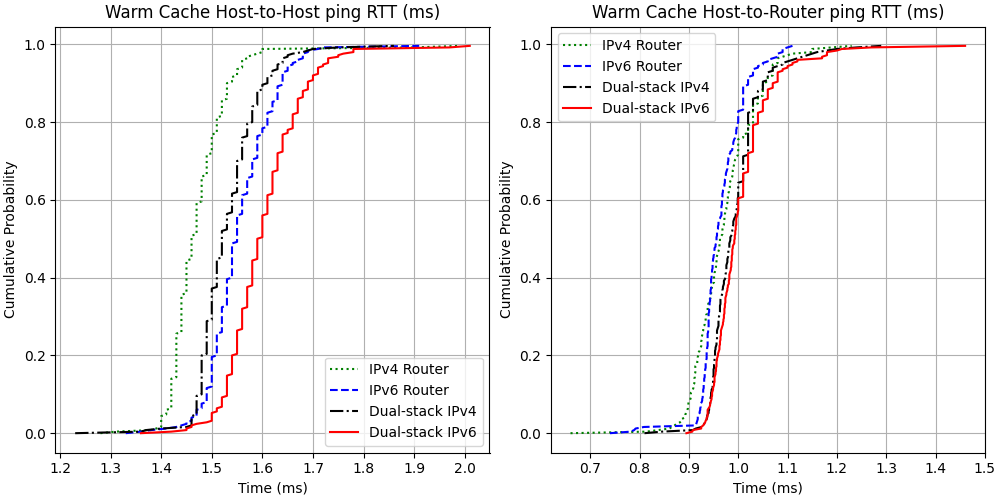
\includegraphics[width=0.90\textwidth]{figures/evaluation/Ping_WC.png}
     \caption{Distributions of warm cache ping RTTs on different configurations when \\ running host-to-host (left) and host-to-router (right).}
     \label{fig:eval-pingWC}
\end{figure}

All distributions exhibit similar slopes and variances. The plots support what could be concluded from \cref{table:eval-ping}. No significant difference is seen between IPv4 and IPv6 in the host-to-router scenario, but the IPv6 mean is 71 $\mu$s higher than the IPv4 mean in the host-to-host scenario. The dual-stack prototype, on average, is 45 $\mu$s slower than the respective single-stack RTTs. There are many reasons for this, such as additional parsing and processing checks, a larger data plane configuration, or simply noise. In both cases, the difference in RTT means falls within the confidence intervals, so no definitive conclusions can be drawn.



\subsection{Cold Cache Echo Request/Reply}
\label{sec:4.3.2}

When running the \texttt{ping} command, the RTT of the first Echo Request/Reply pair is always significantly larger than the rest. This is because Address Resolution/Neighbour Discovery is performed to acquire the next-hop MAC address of the IP address the host is attempting to reach. This information allows us to compare the performances of ARP and NDP. \cref{table:eval-pingCC} shows the RTTs of the first pings after MAC address caches are cleared, and \cref{fig:eval-pingCC} illustrates the collected cold cache data samples as cumulative distribution functions.

\begin{table}[htbp]
    \centering
    \renewcommand{\arraystretch}{1.25}
    \begin{tabular}{|c|c|c|c|c|}
    \hline
    \multirow{2}{*}{\textbf{IP Protocol}} & \multicolumn{2}{c|}{\textbf{Host-to-Host}} & \multicolumn{2}{c|}{\textbf{Host-to-Router}}\\
    \cline{2-5}
     & \textbf{Single-stack} & \textbf{Dual-stack} & \textbf{Single-stack} & \textbf{Dual-stack}\\
    \hline
    IPv4 & 2.770 $\pm$ 0.202 & 2.864 $\pm$ 0.280 & 1.596 $\pm$ 0.244 & 1.748 $\pm$ 0.320 \\
    IPv6 & 3.235 $\pm$ 0.190 & 3.262 $\pm$ 0.240 & 1.746 $\pm$ 0.146 & 1.817 $\pm$ 0.152 \\
    \hline
    \end{tabular}
    \caption{Mean RTT (ms) from 25 cold cache ping commands with a 95\% confidence interval, obtained by adding and subtracting two standard deviations.}
    \label{table:eval-pingCC}
\end{table}

\begin{figure}[htbp]
  \centering
    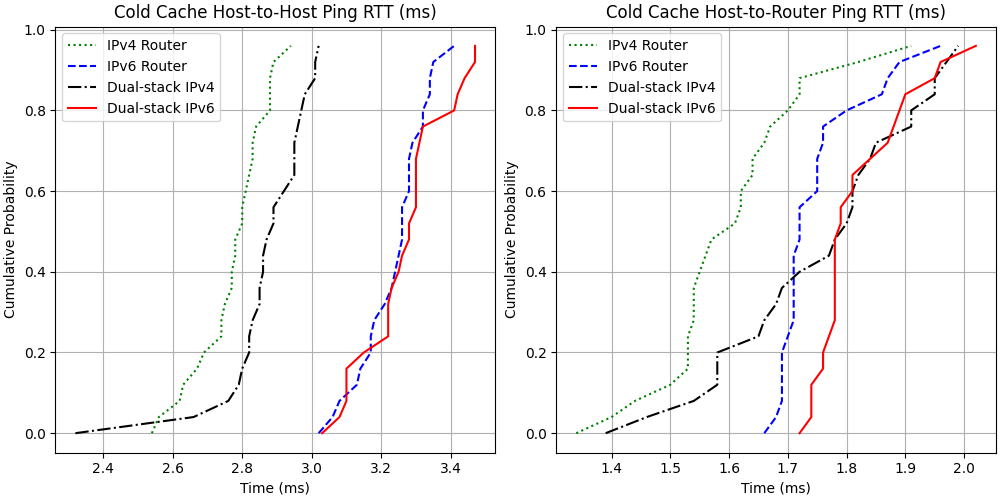
\includegraphics[width=0.90\textwidth]{figures/evaluation/Ping_CC.png}
     \caption{Distributions of cold cache ping RTTs on different configurations when \\ running host-to-host (left) and host-to-router (right).}
     \label{fig:eval-pingCC}
\end{figure}

Observe that IPv6 resolution takes slightly longer than IPv4 resolution. The reason for this is that NDP is part of ICMPv6 and works on top of IPv6, whereas ARP works below IPv4. When developing IPv6, it was decided to integrate NDP into ICMPv6 for efficiency and security reasons which are outside the scope of my dissertation. For the purposes of the gathered results, this means that resolving an NS requires parsing an extra layer of headers, thus takes a margin of time longer than resolving an ARP Request.


\subsection{Performance Summary}
\label{sec:4.3.3}

This section explored the performance of the different router prototypes when simulating identical-purpose traffic in the network. The gathered data shows that the performance of the routers remain stable and suggests that the dual-stack router prototype might be slightly slower than the single-stack routers. NDP is less efficient than ARP, but that is to be expected due to the extra layer of header parsing. Because NDP offers more functionalities than ARP and is only performed once, to establish a connection, the trade-off in efficiency is warranted.

Since any differences in efficiency in the warm cache scenario fall within the confidence intervals, no significant difference in performance can be concluded. Furthermore, the dual-stack router being able to support both IPs greatly benefits networks and outweighs the harm caused by the potentially less efficient packet processing. I thus propose that my router prototypes, both the IPv6 and dual-stack ones, can be used in place of the IPv4 prototype to provide better functionality in a network at a negligible performance cost.



\section{Evaluation Summary}

The evaluation of my project explored correctness, standards compliance and performance. I established that my router prototypes uphold my baseline designs using implementation-driven testing. All design choices were based on observed packet behaviours in working networks. I then compared my router prototypes to the IETF's official specifications and concluded that, for the functionalities that my routers do implement, my routers adhere to the best practices as outlined by the IETF. Finally, I conducted a performance evaluation by running known test traffic in both IPs on both router types (single- and dual-stacked) to establish that there is no significant difference in performance, hence my prototypes can be used in place of the IPv4 prototype to provide better functionality.


\addtocontents{lol}{\protect\vspace*{10pt}}
\chapter{Conclusions}
%TC:envir minted 1 xall 
%TC:envir algorithmic 1 xall

% Include tables in word count
%TC:envir table 0 word
%TC:envir tabular 1 word

% Include footnotes in word count
%TC:macro \footnote [text]
%TC:macro \footnotetext [text]

%TC:group minted 0 0
%TC:macro \mintinline [ignore]
%TC:macro \colb [ignore]
%TC:macro \hyperref [ignore]

\label{sec:5}

This project was motivated by the difficulties posed by the Internet's transition from IPv4 to IPv6. I aimed to build an IPv6 router prototype on a software-defined platform that does not currently support IPv6 and analyse the steps needed to achieve this. I had tentatively hoped to show that my prototype would not impact the performance of a network.


\section{Achievements}
\label{sec:5.1}
This project fulfils its core objectives, along with three proposed extensions. I learned the domain-specific language P4 and how to run P4 programs on the P4Pi platform. I built an IPv6 router prototype that implements parsing, forwarding, longest prefix matching, along with ICMPv6 and NDP functionalities. As my final extension, I combined an IPv4 router prototype with my IPv6 router to implement a dual-stack router prototype, capable of processing packets in both protocols. In \cref{sec:4} I established the correctness of my programs, a high level of adherence to established IETF standards, and stable performance of the IPv6 and dual-stack routers when compared to the IPv4 router. The results gathered during the performance evaluation showed that the routers exhibit no significant change in efficiency when processing known test traffic. This allowed me to tentatively conclude that the migration of software-based IPv4 routers to IPv6 or dual-stack routers is possible without negative impacts on the network, and hopefully outlines a pathway to the more widespread adoption of IPv6 in software switches.

\section{Lessons Learnt}
\label{sec:5.2}

Looking back, I was overly optimistic about how quickly I would acquire the necessary baseline skills to start working on my project. Learning P4 and how to work with P4Pi took much longer than I expected. Once I got into the work, however, I found that the extensions followed naturally from one another, and I did not always need the full two weeks to implement a new functionality. I would benefit in the future to allocate appropriate time for project preparation and planning in order to avoid deviating from my outlined timetable.

\section{Future Work}
\label{sec:5.3}

This project can be expanded upon in many ways, but the most natural next steps would be to implement any remaining ICMPv6 and NDP data plane functionalities that are required by the IETF, but not adopted in my project (as described in \cref{sec:4.2}). Alternatively, the router's control plane could be developed with services such as IP routing protocols, among others. Any further work could involve building networks with more hosts, more subnets, or even by connecting the router to the world wide web.


% ----------------------------------------------------------------------
%TC:ignore
\newpage

\addcontentsline{toc}{chapter}{\numberline{}Bibliography}
\printbibliography

% ----------------------------------------------------------------------

\appendix

\addtocontents{toc}{\protect\setcounter{tocdepth}{0}}

\chapter{Running a P4 Program on the P4Pi Platform}
%TC:envir minted 1 xall 
%TC:envir algorithmic 1 xall

% Include tables in word count
%TC:envir table 0 word
%TC:envir tabular 1 word

% Include footnotes in word count
%TC:macro \footnote [text]
%TC:macro \footnotetext [text]

%TC:group minted 0 0
%TC:macro \mintinline [ignore]
%TC:macro \colb [ignore]
%TC:macro \hyperref [ignore]

Once you have written your P4 program file\texttt{ my\_program.p4}, you must compile it using the p4c compiler and run it on the simple switch target. To do so, go to the location of the P4 file on your P4Pi and run the command:

\begin{quote}
    \texttt{p4c --target bmv2 --arch v1model --std p4-16 my\_program.p4}
\end{quote}

This specifies the behavioural model (bmv2), the model architecture (v1model) and the version of the P4 language that the program is written in (p4-16). The command will generate two new files, \texttt{my\_program.p4i} and \texttt{my\_program.json}. Optionally, you can add another argument to produce a \texttt{.txt} file containing a description of the tables and objects in your P4 program:

\begin{quote}
    \texttt{p4c --target bmv2 --arch v1model --std p4-16 --p4runtime-files my\_program.p4info.txt my\_program.p4}
\end{quote}

Once you have compiled your P4 program, you run it by specifying the implementation of the bmv2 abstract switch that will be used. In this case we are running it on the simple switch target. Use the following command:

\begin{quote} 
    \texttt{simple\_switch -i 0@port0 -i 1@port1 my\_program.json \&}
\end{quote}

The values \texttt{port0} and \texttt{port1} will look similar to \texttt{enx0c37965f8a20}, but to discover the exact values, run \texttt{ip a} on the router and find the addresses of the ports you want to assign your P4 program to use. You can assign any number of interfaces depending on how many ports your program needs.

You can then dynamically modify the P4 tables by running:
\begin{quote}
    \texttt{simple\_switch\_CLI}
\end{quote}
to enter the command-line interface environment, or you can put the commands you want to run in a \texttt{.txt} file and directly feed it into the runtime CLI, as so:
\begin{quote}
    \texttt{simple\_switch\_CLI < commands.txt}
\end{quote}


\chapter{Commands in the CLI}
%TC:envir minted 1 xall 
%TC:envir algorithmic 1 xall

% Include tables in word count
%TC:envir table 0 word
%TC:envir tabular 1 word

% Include footnotes in word count
%TC:macro \footnote [text]
%TC:macro \footnotetext [text]

%TC:group minted 0 0
%TC:macro \mintinline [ignore]
%TC:macro \colb [ignore]
%TC:macro \hyperref [ignore]

The \texttt{simple\_switch\_CLI} gives you the ability to dynamically inspect, add, remove and modify entries in the tables defined by your P4 program. Below are some of the basic commands that can be used.

To show all tables in the program:
\begin{quote}
    \texttt{show\_tables}
\end{quote}

To get information about a table:
\begin{quote}
    \texttt{table\_info tableX}
\end{quote}

To get all entries in a table:
\begin{quote}
    \texttt{table\_dump tableX}
\end{quote}

To add an entry to a table:
\begin{quote}
    \texttt{table\_add tableX actionX 9.9.9.9/32 => aa:bb:cc:dd:ee:ff 0}
\end{quote}

The above example matches an IP address to a MAC address. The \texttt{=>} sign separates the table key from the table action data. The CLI will return a success message that will end with 
\begin{quote}
    \texttt{entry has been added with handle Y}
\end{quote}
The value \texttt{Y} can now be used for all subsequent operations.

To delete an entry:
\begin{quote}
    \texttt{table\_delete tableX Y}
\end{quote}


\chapter{IPv6 Forwarding Experiment}
%TC:envir minted 1 xall 
%TC:envir algorithmic 1 xall

% Include tables in word count
%TC:envir table 0 word
%TC:envir tabular 1 word

% Include footnotes in word count
%TC:macro \footnote [text]
%TC:macro \footnotetext [text]

%TC:group minted 0 0
%TC:macro \mintinline [ignore]
%TC:macro \colb [ignore]
%TC:macro \hyperref [ignore]

You will need three Raspberry Pis: two acting as hosts and one as the router. You will also need two Ethernet cables and two USB-to-Ethernet adapters. Use the cables to connect both your hosts to the router as shown below.

\begin{figure}[htbp]
  \centering
    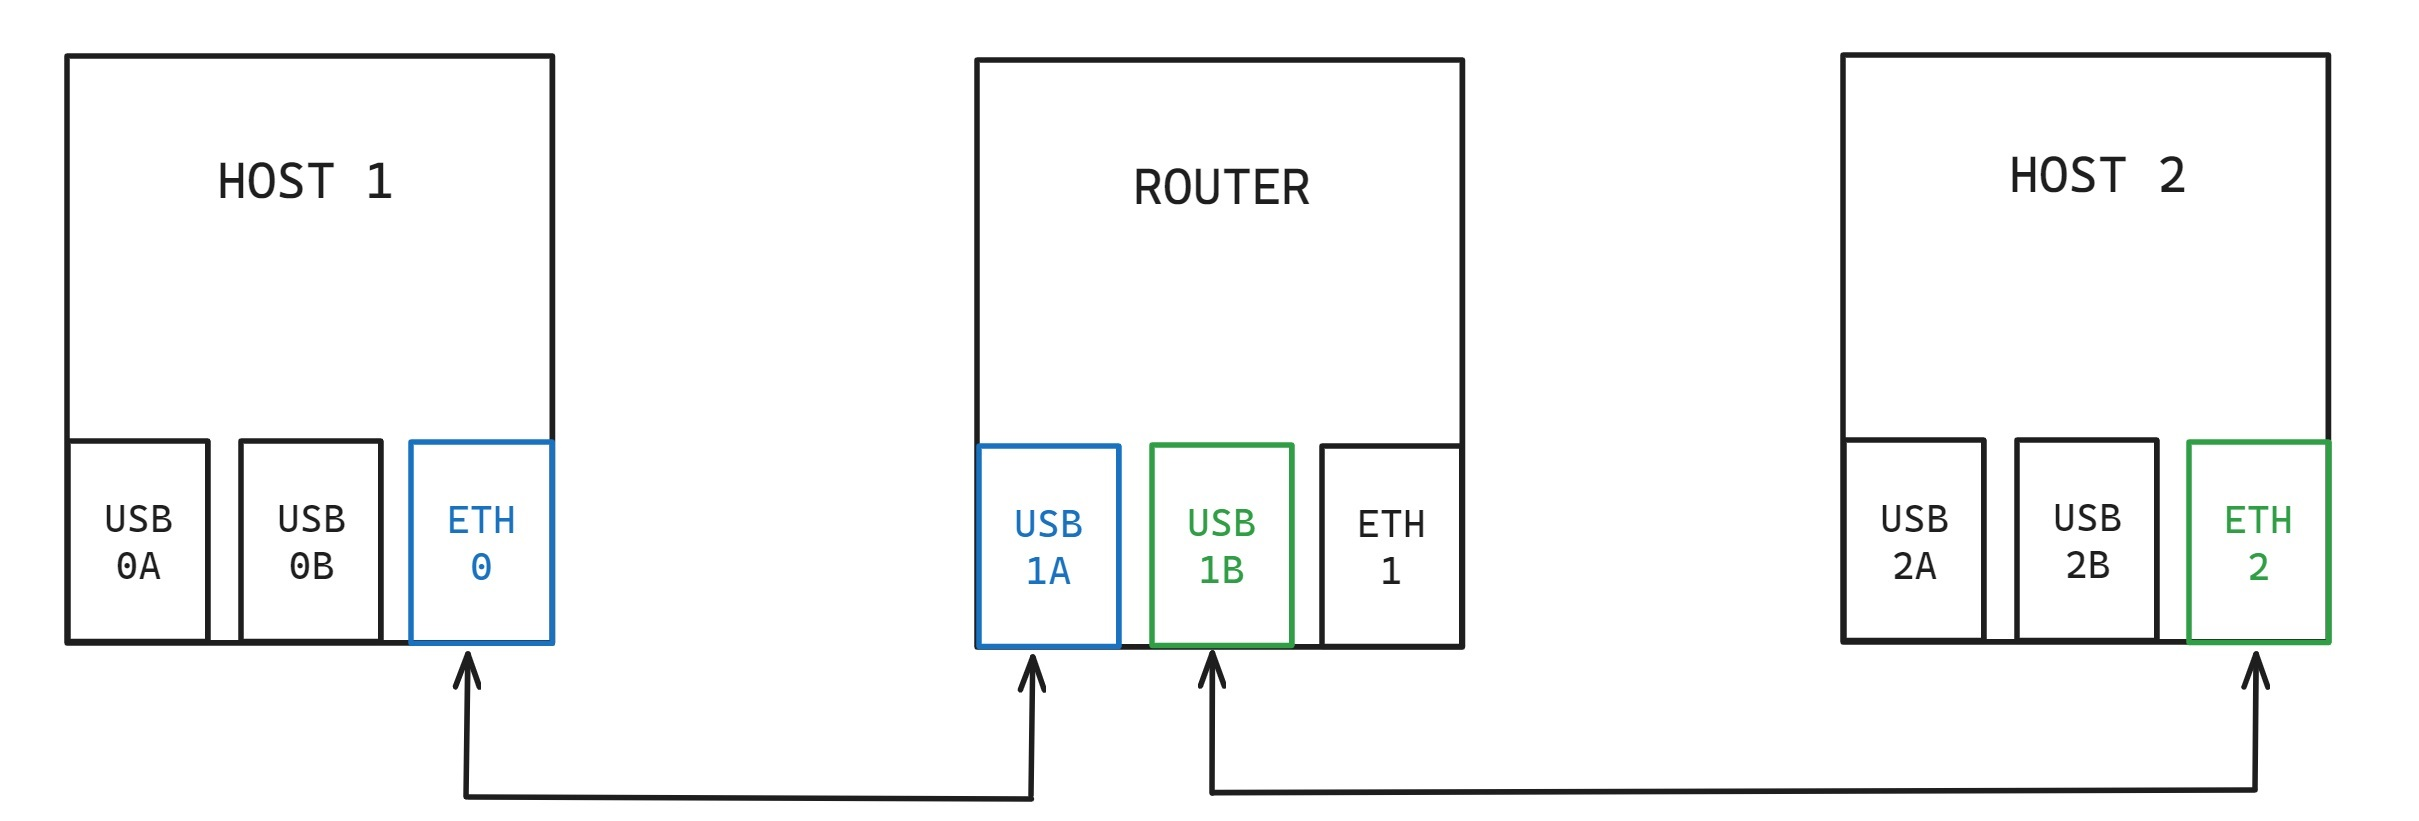
\includegraphics[width=1\textwidth]{figures/appendices/ipv6_setup.jpg}
\end{figure}

Run \texttt{ip a} on the router to learn the MAC and IP addresses of the two USB ports. Choose IPv6 addresses for the hosts such that they are on the same subnet as their corresponding router USB port. Let \texttt{IPa} and \texttt{IPb} denote the chosen IPv6 addresses for Host 1 and Host 2, respectively. On each host, run \texttt{ip a} to learn the MAC address of the host, henceforth referred to as \texttt{MACa} and \texttt{MACb}.

On Host 1, open a command prompt and run:
\begin{quote}
    \texttt{sudo ifconfig eth0 inet6 add IPa}
    
    \texttt{sudo ip -6 route add dev eth0 IPb}
    
    \texttt{sudo ip -6 neigh add dev eth0 IPb lladdr MACb}
\end{quote}

The first line sets a static IPv6 address for Host 1, the second line defines a route to Host 2 and the third line puts an entry in Host 1’s neighbour table, associating Host 2 with a specific MAC address.

Perform the same commands on Host 2:
\begin{quote}
    \texttt{sudo ifconfig eth0 inet6 add IPb}
    
    \texttt{sudo ip -6 route add dev eth0 IPa}
    
    \texttt{sudo ip -6 neigh add dev eth0 IPa lladdr MACa}
\end{quote}

Start the P4 program on the router and, using the CLI (or by using a \texttt{commands.txt} file, as explained in Appendix A), enter the commands:
\begin{quote}
    \texttt{table\_add MyIngress.ipv6\_lpm MyIngress.forward IPa/128 => MACa 0}
    
    \texttt{table\_add MyIngress.ipv6\_lpm MyIngress.forward IPb/128 => MACb 1}
\end{quote}

The \texttt{/128} network identifier prefix tells the router to only forward packets whose destination address matches exactly. This value can be changed to instruct the router to forward packets whose IPv6 address matches to any chosen bit size (i.e. perform a fixed-size prefix match, which can be extended to a longest prefix match).

On Host 1, run the command to send an Echo Request to Host 2:
\begin{quote}
    \texttt{ping6 -I eth0 IPb}
\end{quote}

Host 1 should be receiving Echo Replies from Host 2.

\chapter{ICMPv6 Experiment}
%TC:envir minted 1 xall 
%TC:envir algorithmic 1 xall

% Include tables in word count
%TC:envir table 0 word
%TC:envir tabular 1 word

% Include footnotes in word count
%TC:macro \footnote [text]
%TC:macro \footnotetext [text]

%TC:group minted 0 0
%TC:macro \mintinline [ignore]
%TC:macro \colb [ignore]
%TC:macro \hyperref [ignore]

You will need three Raspberry Pis: two acting as hosts and one as the router. You will also need two Ethernet cables and two USB-to-Ethernet adapters. Use the cables to connect both your hosts to the router as shown below. Static router addresses have been defined by the P4 program.

\begin{figure}[htbp]
  \centering
    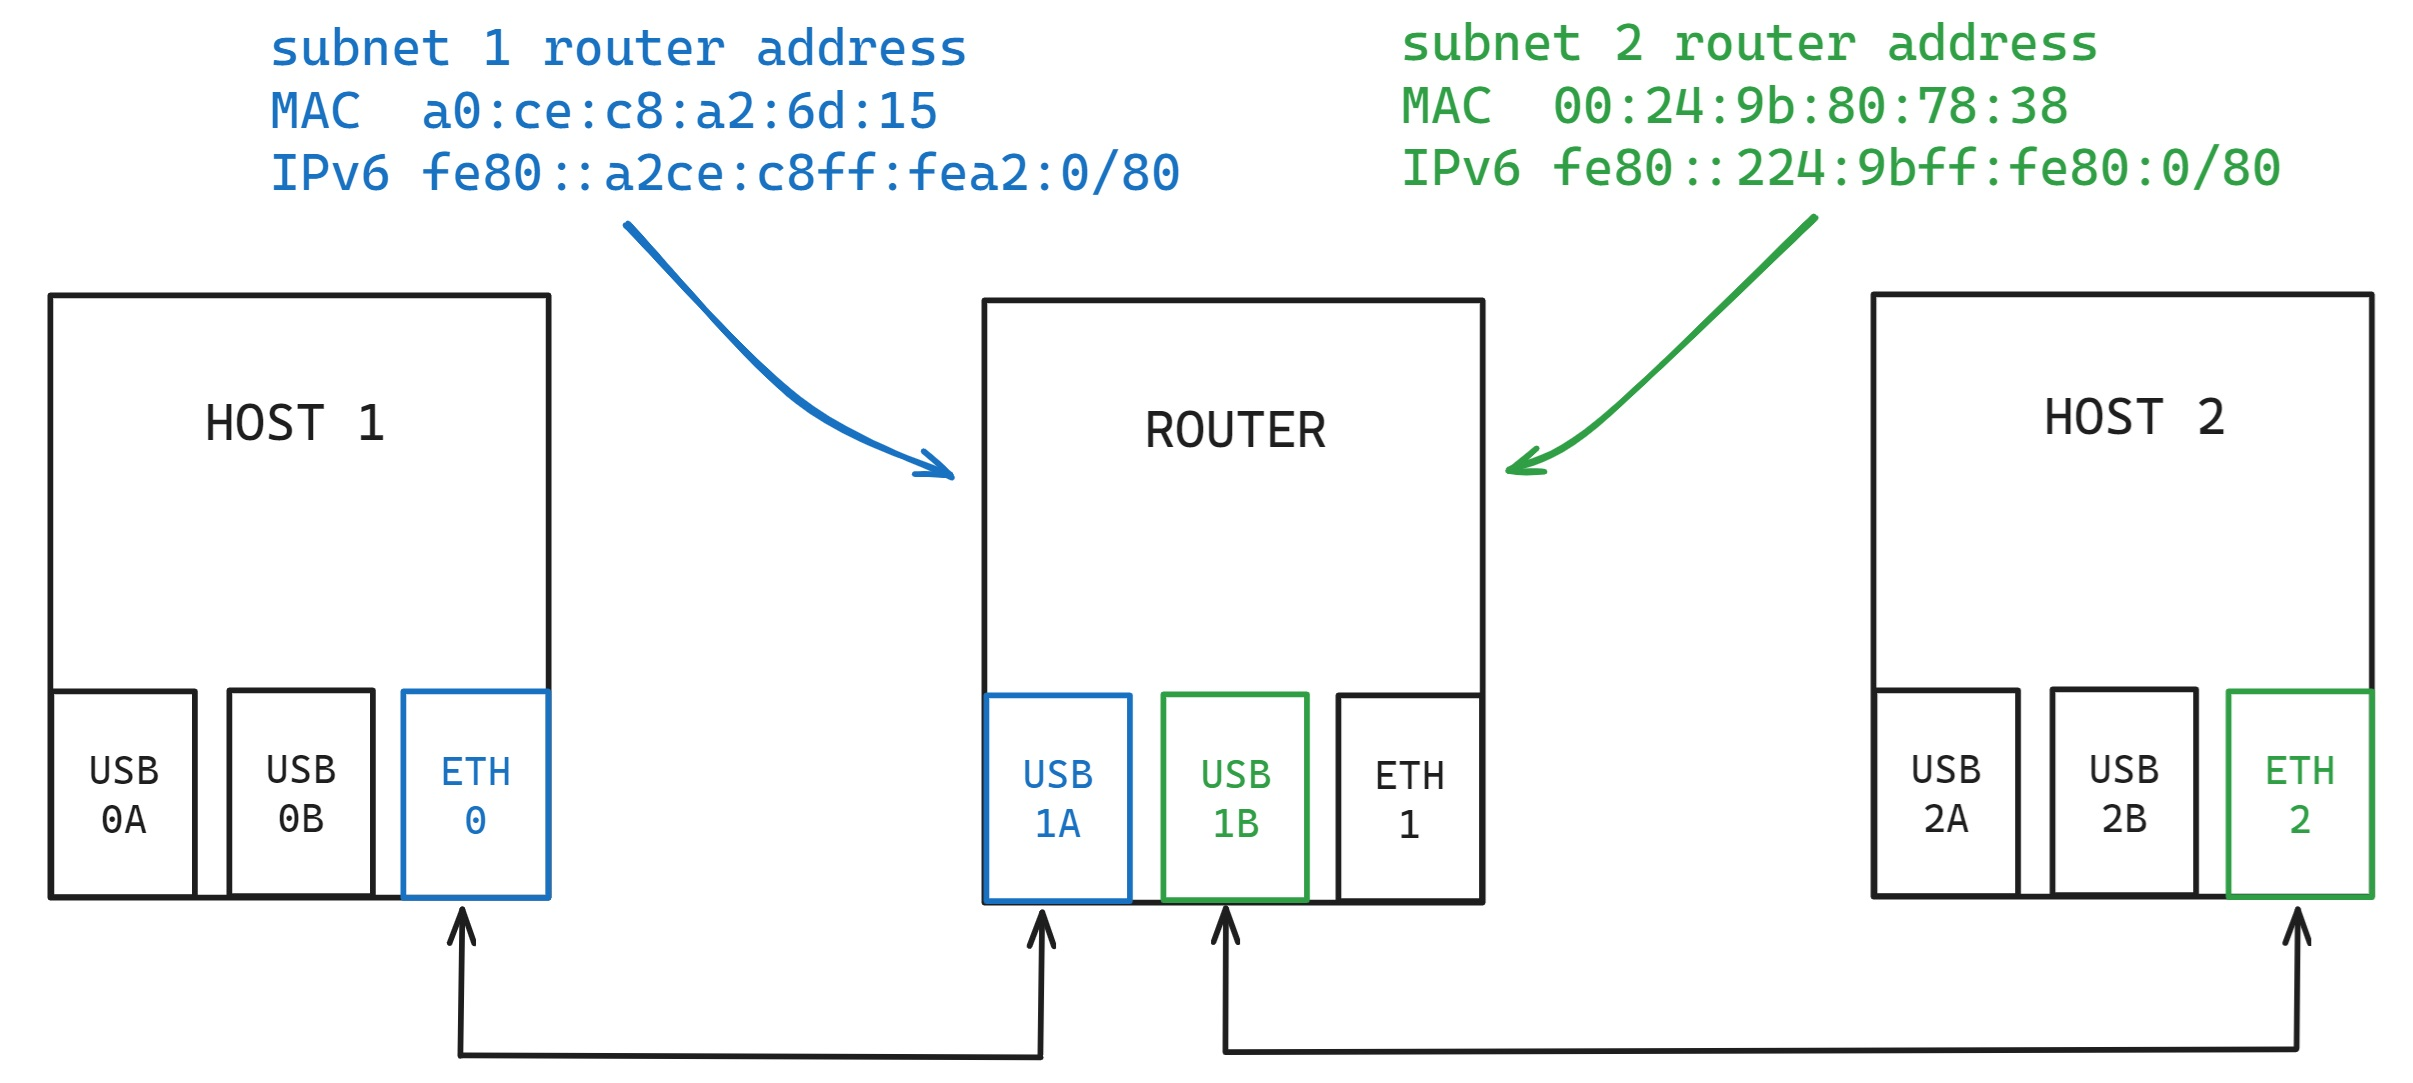
\includegraphics[width=1\textwidth]{figures/appendices/icmpv6_ndp_setup.jpg}
\end{figure}

Run \texttt{ip a} on the router to learn the MAC and IP addresses of the USB ports connected to your hosts. Edit the P4 program to define constant static router IPv6 and MAC addresses (at the top of the program) such that you have one entry for each subnet. These will be referred to as \texttt{IPra}, \texttt{MACra} and \texttt{IPrb}, \texttt{MACrb}. The MAC addresses should match the router’s port MAC addresses, and the IP addresses should belong to the same subnets as the ports. 

Choose IPv6 addresses \texttt{IPa} and \texttt{IPb} for the hosts such that they belong to the same subnet as their respective router USB ports. Also run \texttt{ip a} on the hosts to learn their MAC addresses \texttt{MACa} and \texttt{MACb}.

On Host 1, open a command prompt and run:
\begin{quote}
    \texttt{sudo ifconfig eth0 inet6 add IPa}
    
    \texttt{sudo ip -6 route add dev eth0 IPra}
    
    \texttt{sudo ip -6 neigh add dev eth0 IPra lladdr MACra}
\end{quote}

The first line sets a static IPv6 address on Host 1, the second line defines a route to the static address and the third line puts an entry in Host 1’s neighbour table, associating the router IPv6 address with the specified router MAC address.

Run the same commands on Host 2:
\begin{quote}
    \texttt{sudo ifconfig eth0 inet6 add IPb}
    
    \texttt{sudo ip -6 route add dev eth0 IPrb}
    
    \texttt{sudo ip -6 neigh add dev eth0 IPrb lladdr MACrb}
\end{quote}

Start the P4 program on the router using the port connected to Host 1. Then, run the \texttt{ping} command on Host 1:
\begin{quote}
    \texttt{ping6 -I eth0 IPra}
\end{quote}

Or on Host 2: 
\begin{quote}
    \texttt{ping6 -I eth0 IPrb}
\end{quote}

These should generate an Echo Reply from the respective router addresses. To receive a Time Exceeded error message, use an additional argument to set the hop limit to 1, e.g.:
\begin{quote}
    \texttt{ping6 -I eth0 IPra -t 1}
\end{quote}

If you define a route and MAC neighbour entry to a random address and then direct an Echo Request towards it, you should receive a Destination Unreachable error message from the router.


\chapter{NDP Experiment}
%TC:envir minted 1 xall 
%TC:envir algorithmic 1 xall

% Include tables in word count
%TC:envir table 0 word
%TC:envir tabular 1 word

% Include footnotes in word count
%TC:macro \footnote [text]
%TC:macro \footnotetext [text]

%TC:group minted 0 0
%TC:macro \mintinline [ignore]
%TC:macro \colb [ignore]
%TC:macro \hyperref [ignore]

You will need three Raspberry Pis: two acting as hosts and one as the router. You will also need two Ethernet cables and two USB-to-Ethernet adapters. Use the cables to connect both your hosts to the router as shown below. Static router addresses have been defined by the P4 program.

\begin{figure}[htbp]
  \centering
    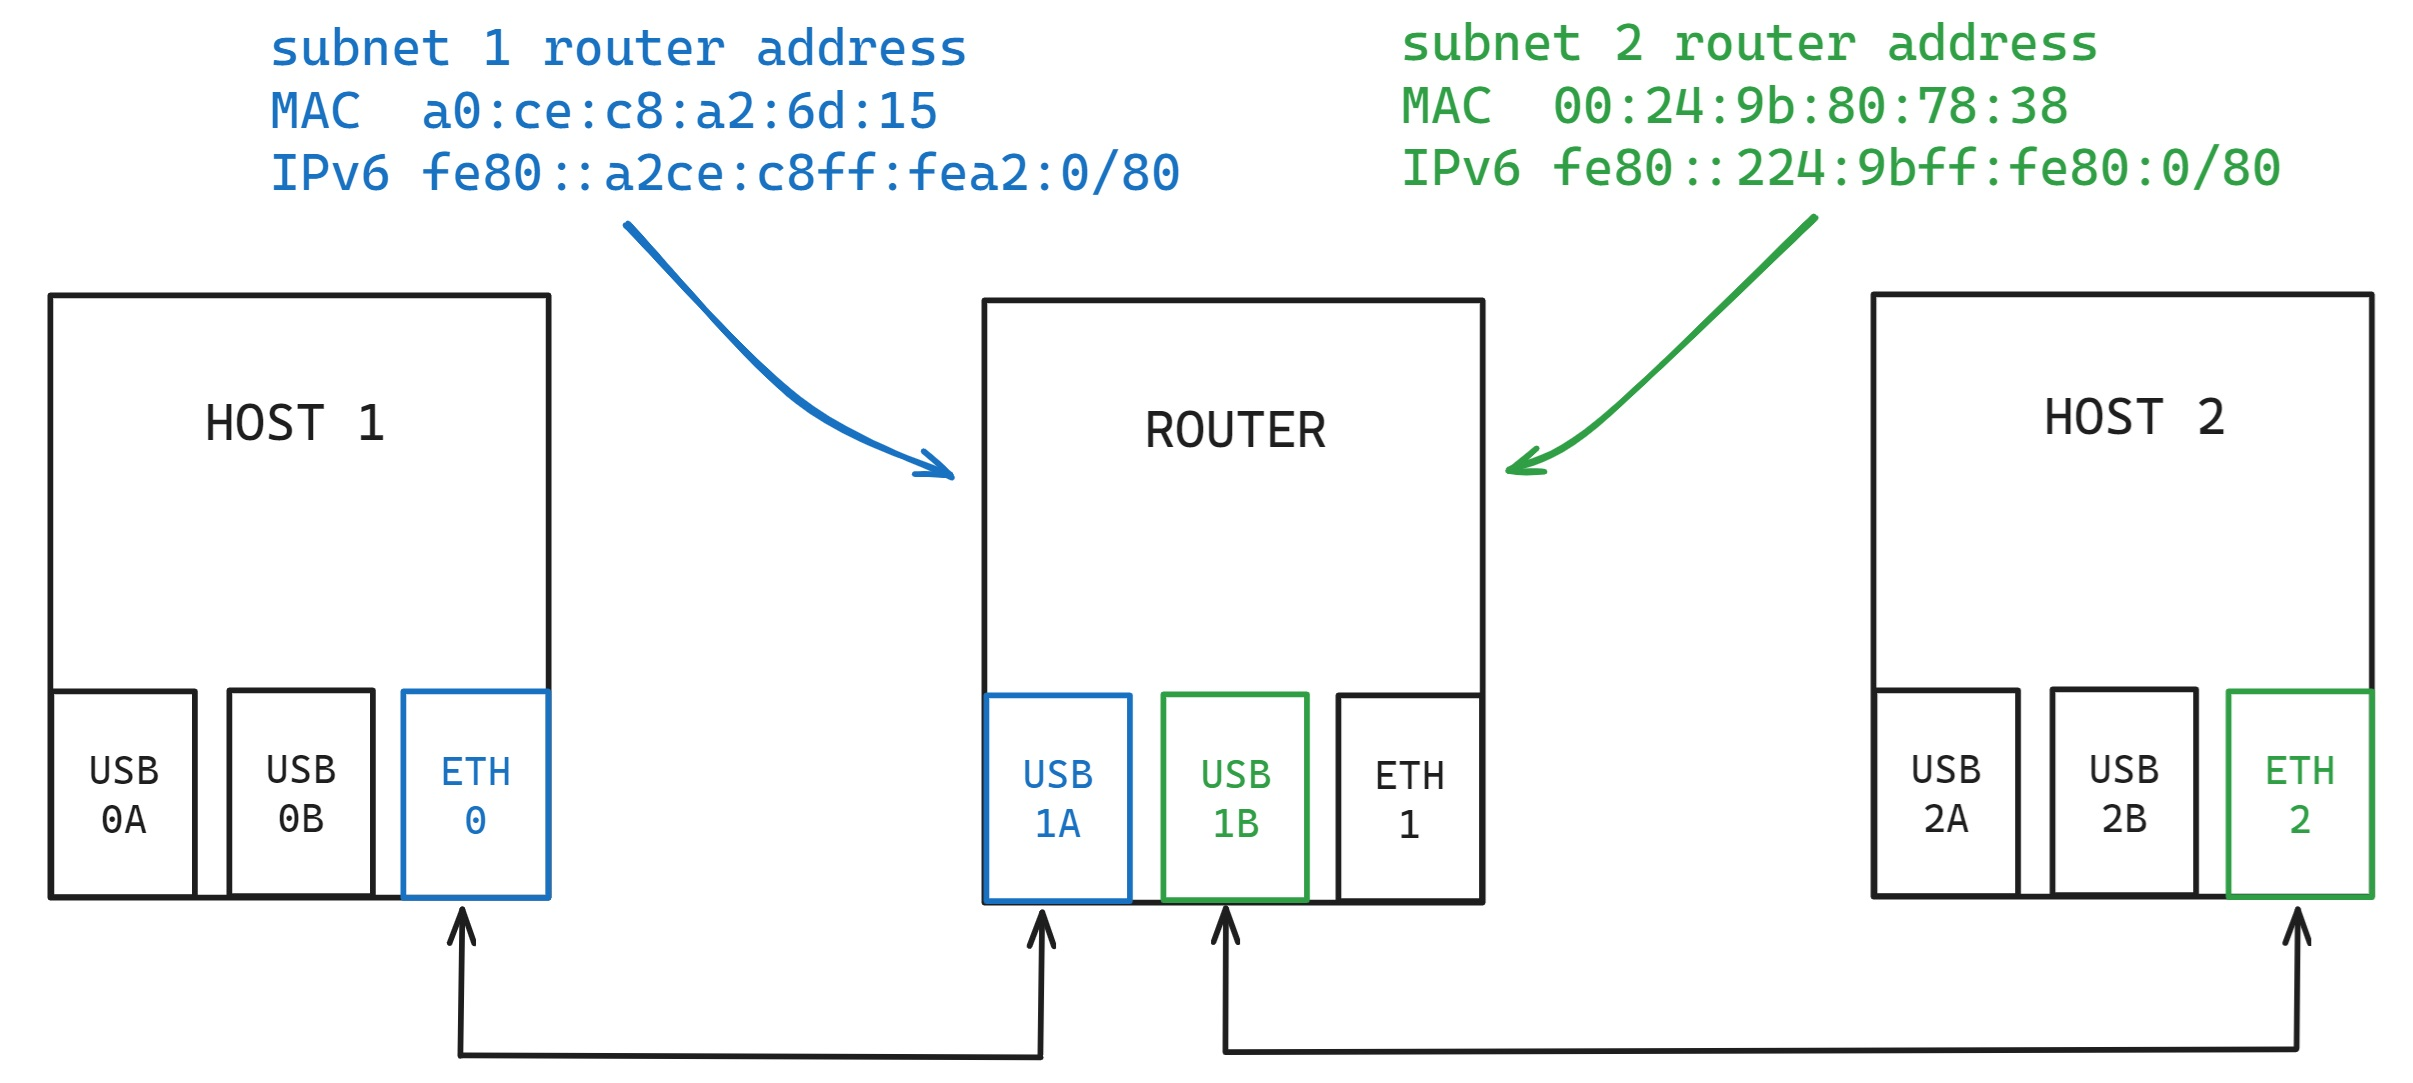
\includegraphics[width=1\textwidth]{figures/appendices/icmpv6_ndp_setup.jpg}
\end{figure}

Run \texttt{ip a} on the router to learn the MAC and IP addresses of the USB ports connected to your hosts. Edit the P4 program to define constant static router IPv6 and MAC addresses (at the top of the program) such that you have one entry for each subnet. These will be referred to as \texttt{IPra}, \texttt{MACra} and \texttt{IPrb}, \texttt{MACrb}. The MAC addresses should match the router’s port MAC addresses, and the IP addresses should belong to the same subnets as the ports. 

Choose IPv6 addresses \texttt{IPa} and \texttt{IPb} for the hosts such that they belong to the same subnet as their respective router USB ports. Also run \texttt{ip a} on the hosts to learn their MAC addresses \texttt{MACa} and \texttt{MACb}.

On Host 1, open a command prompt and run:
\begin{quote}
    \texttt{sudo ifconfig eth0 inet6 add IPa}
    
    \texttt{sudo ip -6 route add dev eth0 IPra}
    
    \texttt{sudo ip -6 neigh show}
\end{quote}

The first line sets a static IPv6 address on Host 1 and the second line defines a route to the static address. The third line prints out all entries in the host’s neighbour table. It should be initially empty.

Start the P4 program on the router using the port connected to Host 1. Start up the CLI and enter the commands (or run these by using a \texttt{commands.txt} file, as explained in Appendix A):
\begin{quote}
    \texttt{table\_add MyIngress.nei\_responder MyIngress.nei\_adv IPa => MACa 1}
    
    \texttt{table\_add MyIngress.nei\_responder MyIngress.nei\_adv IPb => MACb 2}
    
    \texttt{table\_add MyIngress.nei\_responder MyIngress.nei\_adv IPra => MACra 1}
    
    \texttt{table\_add MyIngress.nei\_responder MyIngress.nei\_adv IPrb => MACrb 2}
\end{quote}

Then, run the \texttt{ping} command on Host 1:
\begin{quote}
    \texttt{ping6 -I eth0 IPra}
\end{quote}
This should not generate any response, as no Echo Reply functionalities have been written into the program. Finally, run:
\begin{quote}
    \texttt{sudo ip -6 neigh show}
\end{quote}

There should now be an entry associating \texttt{IPra} with \texttt{MACra}. Pinging Host 2 should add another entry to the neighbour table. The same commands can be performed on Host 2 to acquire the MAC addresses of the router and Host 1.


\chapter{IPv6 Router Experiment}
%TC:envir minted 1 xall 
%TC:envir algorithmic 1 xall

% Include tables in word count
%TC:envir table 0 word
%TC:envir tabular 1 word

% Include footnotes in word count
%TC:macro \footnote [text]
%TC:macro \footnotetext [text]

%TC:group minted 0 0
%TC:macro \mintinline [ignore]
%TC:macro \colb [ignore]
%TC:macro \hyperref [ignore]

You will need three Raspberry Pis: two acting as hosts and one as the router. You will also need two Ethernet cables and two USB-to-Ethernet adapters. Use the cables to connect both your hosts to the router as shown below. Static router addresses have been defined by the P4 program.

\begin{figure}[htbp]
  \centering
    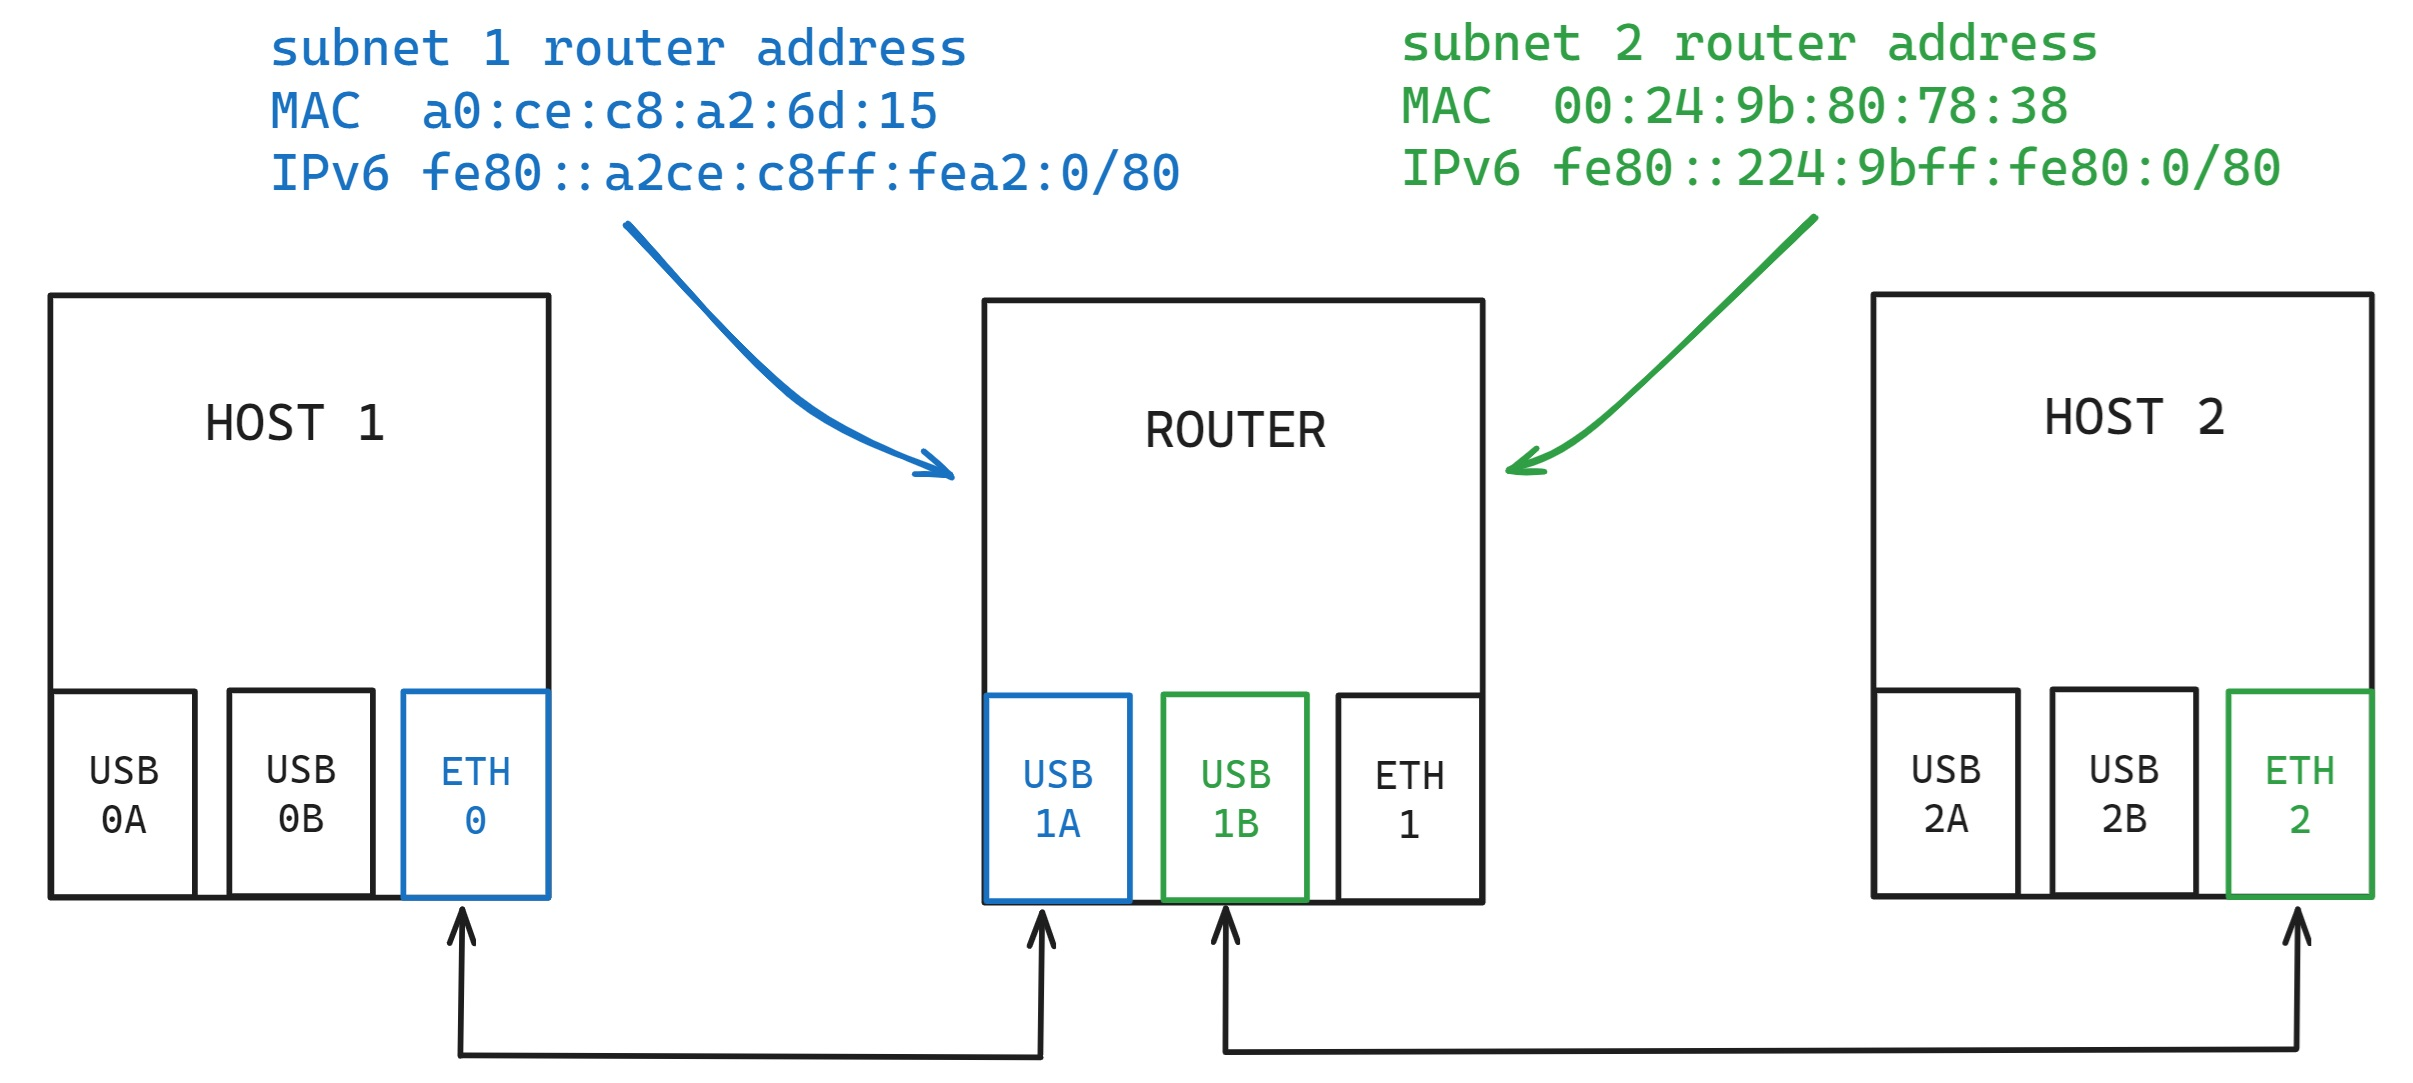
\includegraphics[width=1\textwidth]{figures/appendices/icmpv6_ndp_setup.jpg}
\end{figure}

Run \texttt{ip a} on the router to learn the MAC and IP addresses of the USB ports connected to your hosts. Edit the P4 program to define constant static router IPv6 and MAC addresses (at the top of the program) such that you have one entry for each subnet. These will be referred to as \texttt{IPra}, \texttt{MACra} and \texttt{IPrb}, \texttt{MACrb}. The MAC addresses should match the router’s port MAC addresses, and the IP addresses should belong to the same subnets as the ports. 

Choose IPv6 addresses \texttt{IPa} and \texttt{IPb} for the hosts such that they belong to the same subnet as their respective router USB ports. Also run ip a on the hosts to learn their MAC addresses \texttt{MACa} and \texttt{MACb}.

On Host 1, open a command prompt and run:
\begin{quote}
    \texttt{sudo ifconfig eth0 inet6 add IPa}
    
    \texttt{sudo ip -6 route add dev eth0 IPra}
    
    \texttt{sudo ip -6 route add dev eth0 IPb}
    
    \texttt{sudo ip -6 neigh show}
\end{quote}

The first line sets a static IPv6 address for Host 1, the second line defines a route to the router and the third line defines a route to Host 2. The fourth line outputs the neighbour entry table, which should initially be empty. 

Run the same commands on Host 2:
\begin{quote}
    \texttt{sudo ifconfig eth0 inet6 add IPb}

    \texttt{sudo ip -6 route add dev eth0 IPrb}

    \texttt{sudo ip -6 route add dev eth0 IPa}
    
    \texttt{sudo ip -6 neigh show}
\end{quote}

Start the P4 program on the router and, using the CLI (or by using a \texttt{commands.txt} file, as explained in Appendix A), enter the following five commands:

\begin{quote}
    \texttt{table\_add MyIngress.ipv6\_lpm MyIngress.forward IPa/128 => MACa 0}
    
    \texttt{table\_add MyIngress.ipv6\_lpm MyIngress.forward IPb/128 => MACb 1}
    
    \texttt{table\_add MyIngress.nei\_responder MyIngress.nei\_adv IPa => MACa 1}
    
    \texttt{table\_add MyIngress.nei\_responder MyIngress.nei\_adv IPb => MACb 2}
    
    \texttt{table\_add MyIngress.nei\_responder MyIngress.nei\_adv IPra => MACra 1}
    
    \texttt{table\_add MyIngress.nei\_responder MyIngress.nei\_adv IPrb => MACrb 2}
\end{quote}

To test IPv6 forwarding, on Host 1, run the command to ping Host 2:
\begin{quote}
    \texttt{ping6 -I eth0 IPb}
\end{quote}

To test the ICMPv6 Echo Reply, on Host 1, run the command to ping the router:
\begin{quote}
    \texttt{ping6 -I eth0 IPra}
\end{quote}

To test the ICMPv6 time exceeded error message, run the command to ping either the other host or the router, with hop limit set to one:
\begin{quote}
    \texttt{ping6 -I eth0 IPrb -t 1}
\end{quote}

If you define a route and MAC neighbour entry to a random address and then direct an Echo Request towards it, you should receive a Destination Unreachable error message from the router.

To check that neighbour solicitation and advertisement is working properly, output the neighbour table on a host after attempting to ping an address:
\begin{quote}
    \texttt{ping6 -I eth0 IPra}
    
    \texttt{sudo ip -6 neigh show}
\end{quote}

The equivalent commands can be performed on Host 2 to achieve the same results.

\chapter{Dual-Stack Router Experiment}
%TC:envir minted 1 xall 
%TC:envir algorithmic 1 xall

% Include tables in word count
%TC:envir table 0 word
%TC:envir tabular 1 word

% Include footnotes in word count
%TC:macro \footnote [text]
%TC:macro \footnotetext [text]

%TC:group minted 0 0
%TC:macro \mintinline [ignore]
%TC:macro \colb [ignore]
%TC:macro \hyperref [ignore]

You will need three Raspberry Pis: two acting as hosts and one as the router. You will also need two Ethernet cables and two USB-to-Ethernet adapters. Use the cables to connect both your hosts to the router as shown below. Static router addresses have been defined by the P4 program.

\begin{figure}[htbp]
  \centering
    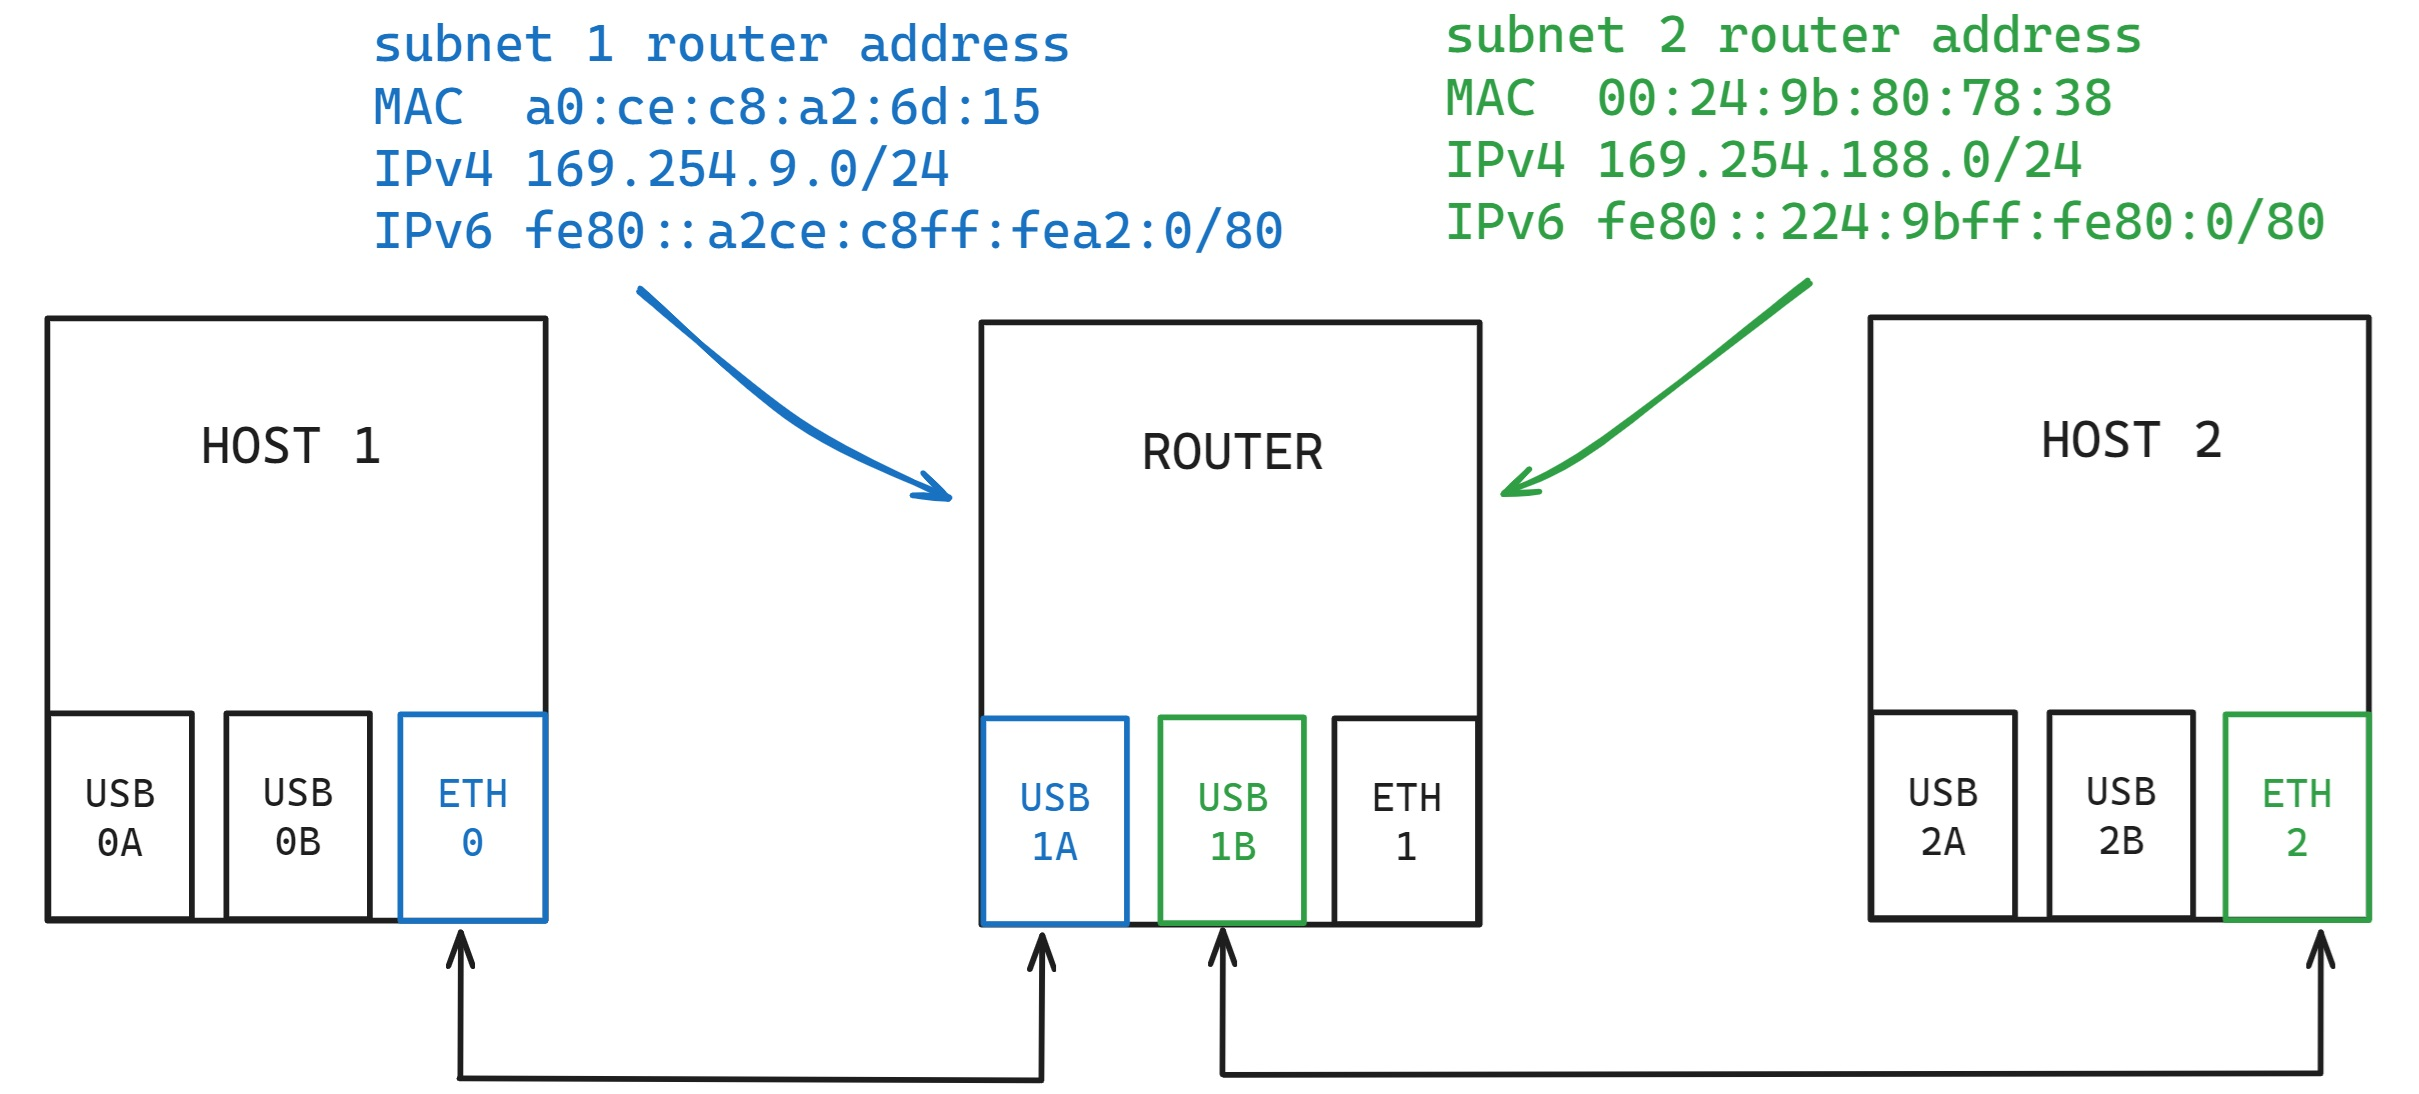
\includegraphics[width=1\textwidth]{figures/appendices/dualstack_setup.jpg}
\end{figure}

Run \texttt{ip a} on the router to learn the MAC and IP addresses of the USB ports connected to your hosts. Edit the P4 program to define constant static router IPv4, IPv6 and MAC addresses (at the top of the program) such that you have one entry for each subnet. These will be referred to as \texttt{IPV4ra}, \texttt{IPV6ra}, \texttt{MACra} and \texttt{IPV4rb}, \texttt{IPV6rb}, \texttt{MACrb}. The MAC addresses should match the router’s port MAC addresses, and the IP addresses should belong to the same subnets as the ports. 

Choose IP addresses \texttt{IPV4a}, \texttt{IPV6a} and \texttt{IPV4b}, \texttt{IPV6b} for the hosts such that they belong to the same subnet as their respective router USB ports. Also run \texttt{ip a} on the hosts to learn their MAC addresses \texttt{MACa} and \texttt{MACb}.

On Host 1, open a command prompt and run the following commands.

To set the host’s IP addresses:
\begin{quote}
    \texttt{sudo ifconfig eth0 IPv4a}
    
    \texttt{sudo ifconfig eth0 inet6 add IPv6a}
\end{quote}

To add routes from Host 1 to the router:
\begin{quote}
    \texttt{sudo ip route add dev eth0 IPv4ra}
    
    \texttt{sudo ip -6 route add dev eth0 IPv6ra}
\end{quote}

To add routes from Host 1 to Host 2:
\begin{quote}
    \texttt{sudo ip route add dev eth0 IPv4b}
    
    \texttt{sudo ip -6 route add dev eth0 IPv6b}
\end{quote}

To check neighbour entry tables (they should initially be empty on port \texttt{eth0}):
\begin{quote}
    \texttt{sudo arp -a}
    
    \texttt{sudo ip -6 neigh show}
\end{quote}

Run the same commands on Host 2, swapping all addresses of Host 1 and Host 2, and using subnet 2’s router address instead of subnet 1’s.

Start the P4 program on the router and, using the CLI (or by using a \texttt{commands.txt} file, as explained in Appendix A), enter the following six commands to populate the IPv4 tables:
\begin{quote}
    \texttt{table\_add MyIngress.ipv4\_lpm MyIngress.forward IPV4a/32 => MACa 0}

    \texttt{table\_add MyIngress.ipv4\_lpm MyIngress.forward IPV4b/32 => MACb 1}
    
    \texttt{table\_add MyIngress.arp\_responder MyIngress.arp\_reply IPV4a => MACa}
    
    \texttt{table\_add MyIngress.arp\_responder MyIngress.arp\_reply IPV4b => MACb}

    \texttt{table\_add MyIngress.arp\_responder MyIngress.arp\_reply IPV4ra => MACra}

    \texttt{table\_add MyIngress.arp\_responder MyIngress.arp\_reply IPV4rb => MACrb}
\end{quote}

And enter the following six commands to populate the IPv6 tables:
\begin{quote}
    \texttt{table\_add MyIngress.ipv6\_lpm MyIngress.forward IPV6a/128 => MACa 0}
    
    \texttt{table\_add MyIngress.ipv6\_lpm MyIngress.forward IPV6b/128 => MACb 1}
    
    \texttt{table\_add MyIngress.nei\_responder MyIngress.nei\_adv IPV6a => MACa 1}
    
    \texttt{table\_add MyIngress.nei\_responder MyIngress.nei\_adv IPV6b => MACb 2}
    
    \texttt{table\_add MyIngress.nei\_responder MyIngress.nei\_adv IPV6ra => MACra 1}
    
    \texttt{table\_add MyIngress.nei\_responder MyIngress.nei\_adv IPV6rb => MACrb 2}
\end{quote}

To test IP forwarding, on Host 1, run the command to ping Host 2:
\begin{quote}
    \texttt{ping IPv4b}
    
    \texttt{ping6 -I eth0 IPv6b}
\end{quote}

To test the ICMPv6 Echo Reply, on Host 1, run the command to ping the router:
\begin{quote}
    \texttt{ping IPv4ra}
    
    \texttt{ping6 -I eth0 IPv6ra}
\end{quote}

To test the ICMPv6 Time Exceeded error message, on either host, run the command to ping either the other host or the router, with hop limit set to one, e.g.:
\begin{quote}
    \texttt{ping6 -I eth0 IPra -t 1}
\end{quote}

This functionality was not implemented in the original IPv4 router, so an equivalent ICMPv4 test will not yield any response. 

Similarly, if you direct an Echo Request towards any other defined IPv6 address (you would need to add both a route and a neighbour table entry to this address first), you should receive an ICMPv6 Destination Unreachable error message, but not if you direct it towards an IPv4 address.

To check that neighbour solicitation and advertisement is working properly, output the neighbour table on a host after attempting to ping an address:
\begin{quote}
    \texttt{ping IPv4ra}
    
    \texttt{sudo arp -a}
    
    \texttt{ping6 -I eth0 IPra}
    
    \texttt{sudo ip -6 neigh show}
\end{quote}

\chapter{Project Proposal}
%TC:envir minted 1 xall 
%TC:envir algorithmic 1 xall

% Include tables in word count
%TC:envir table 0 word
%TC:envir tabular 1 word

% Include footnotes in word count
%TC:macro \footnote [text]
%TC:macro \footnotetext [text]

%TC:group minted 0 0
%TC:macro \mintinline [ignore]
%TC:macro \colb [ignore]
%TC:macro \hyperref [ignore]

The dissertation title has been updated to better reflect the nature of the project.


% don't forget to append the original project proposal
%TC:endignore
\end{document}